\documentclass[a4paper,BCOR7mm,12pt,headsepline,pointlessnumbers,bibtotoc]{scrbook}
% Standard-Dokument mit
%   Papierformat A4
%   Binderand 7 mm
%   Schrift 12-Punkt
%   Linie unter der Kopfzeile
%   Nummern ohne Punkt am Ende
%   Literaturverzeichnis mit Nummer im Inhaltverzeichnis

% bunte tabellen
\usepackage{colortbl}
\usepackage[table]{xcolor}
\definecolor{Gray}{gray}{0.9}
\definecolor{hellgrau}{gray}{0.55}

\let\ttfamilyorg\ttfamily
\renewcommand\ttfamily{\small\ttfamilyorg}

\usepackage{nassi}   

% Define German as thesis language
%\usepackage{german}

\usepackage{tabularx}
\newcolumntype{L}[1]{>{\arraybackslash}p{#1}}

%\usepackage{ngerman}
\usepackage[ngerman]{babel}

% Codierung
\usepackage[latin1]{inputenc}

% kein einrueckungen
\parindent 0pt

% zusaetzliche Symbole
\usepackage{textcomp, latexsym}

% Grafiken
% \usepackage{graphicx, psfrag}
%\usepackage[dvips]{graphics}
\usepackage{graphicx}

% "H"-Option f�r Gleitumgebungen
\usepackage{float}

% Gleitumgebungen nach Referenz platzieren
% \usepackage{flafter}

%\usepackage{attachfile}

% lange Tabellen
\usepackage{longtable}

% Quellcode
\usepackage{listings}

\makeindex


%Mathematik
\usepackage{amsmath}
\usepackage{amsfonts}
\usepackage{amssymb}
\DeclareMathSizes{9}{18}{12}{8}   % For size 10 text 

\usepackage{index}
\newindex{default}{idx}{ind}{Index}

% neue deutsche Rechtschreibung
%\usepackage{german}

% nummerierungs tiefe
\setcounter{secnumdepth}{2}

% Absatzabstand etwas groesser
% \addtolength{\parskip}{1.3ex}

% Blocksatz erzwingen
\sloppy

% Abstand zweier Listenelemente kleiner
\setlength{\itemsep}{0ex plus0.2ex}

% "Rahmenabstand" f�r gerahmte Gleichungen
\setlength{\fboxsep}{10pt}


%\usepackage[english]{babel} %language selection
%\selectlanguage{english}

\pagenumbering{arabic}

%\usepackage{hyperref}
%\hypersetup{colorlinks, 
%citecolor=black,
%filecolor=black,
%linkcolor=black,
%urlcolor=black,
%bookmarksopen=true,
%pdftex}

\hfuzz = .6pt % avoid black boxes

% Befehle zum setzen des Arbeitstyps, Titels, etc...
\newcommand{\selectedthesistype}{}
\newcommand{\thesistype}[1]{\renewcommand{\selectedthesistype}{#1}}
\newcommand{\selectedthesistitle}{}
\newcommand{\thesistitle}[1]{\renewcommand{\selectedthesistitle}{#1}}
\newcommand{\selectedthesisauthor}{}
\newcommand{\thesisauthor}[1]{\renewcommand{\selectedthesisauthor}{#1}}
\newcommand{\selectedthesisdate}{}
\newcommand{\thesisdate}[1]{\renewcommand{\selectedthesisdate}{#1}}
\newcommand{\selectedthesisadvisor}{}
\newcommand{\thesisadvisor}[1]{\renewcommand{\selectedthesisadvisor}{#1}}
\newcommand{\selectedthesisstart}{}
\newcommand{\thesisstart}[1]{\renewcommand{\selectedthesisstart}{#1}}
\newcommand{\selectedthesisend}{}
\newcommand{\thesisend}[1]{\renewcommand{\selectedthesisend}{#1}}

% Leere gerade Seiten sollen keinen Header haben --------------------
\makeatletter
\def\cleardoublepage{\clearpage\if@twoside \ifodd\c@page\else
  \hbox{}
  \thispagestyle{empty}
  \newpage
  \if@twocolumn\hbox{}\newpage\fi\fi\fi}
\makeatother
% -------------------------------------------------------------------

% Trennungsausnahmen-------------------------------------------------
% \hyphenation{}

%
% Und hier geht es los
\begin{document}

    \frontmatter % mit kleinen roemischen Seitenzahlen
% ==========================================================
% Deckblatt erstellen
% ==========================================================
\begin{titlepage}
	\setlength{\topmargin}{-35mm}
	\setlength{\marginparsep}{-55mm}
	\setlength{\marginparwidth}{-55mm}
	\setlength{\textheight}{290mm}
	\setlength{\textwidth}{200mm}
	\enlargethispage{290mm}
	%\setlength{\footskip}{0mm}
	%\setlength{\footheight}{0mm}
		\begin{flushright}
			\begin{tabular}{>{\LARGE}m{120mm}m{45cm}}
				\textbf{\Huge{\textcolor{hellgrau}{Diplomarbeit}}}
				&	
				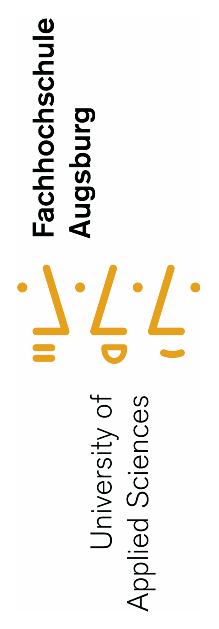
\includegraphics{fha_dpl_ct_logo} \\
				Studienrichtung
			 	& \\
				\vspace{0.5cm}
				Informatik
				& \\
				\vspace{2cm}
				\textbf{Benedikt Sauter} \\
				& \\
				USB-Stack f�r Embedded-Systeme
				& \\
			\end{tabular}
		\end{flushright}
		\begin{tabular}{>{\LARGE}m{130mm}>{\scriptsize}m{50mm}}
			Erstpr�fer: Prof. Dr. Hubert H�gl \newline
			Zweitpr�fer: Prof. Dr. Gundolf Kiefer \newline
			Abgabe der Arbeit: 16.07.2007					
			& 
			Verfasser der Diplomarbeit: \newline
			Benedikt Sauter \newline
			Ketteng�sschen 6 \newline
			86152 Augsburg \newline
			sauter@ixbat.de \newline
			\newline
			Fakult�t \newline
			Informatik \newline
			Telefon: +49 821 5586-450 \newline
			Fax:       +49 821 5586-499 \newline
			\newline
			Fachhochschule Augsburg \newline
			University of Applied Sciences \newline
			Baumgartnerstra�e 16 \newline
			D 86161 Augsburg \newline
			\newline				
			Telefon +49 821 5586-0 \newline
			Fax +49 821 5586-222 \newline
			www.fh-augsburg.de \newline
			poststelle@fh-augsburg.de \newline
		\end{tabular}
\end{titlepage}


    %\maketitle
    \newpage

\thispagestyle{empty}
\markright{Erkl�rung}
\cleardoublepage
\vspace*{9cm}

Ich erkl�re hiermit, dass ich die Arbeit selbstst�ndig verfasst, noch nicht anderweitig f�r Pr�fungszwecke vorgelegt, keine anderen als die angegebenen Quellen oder Hilfsmittel benutzt sowie w�rtliche und sinngem��e Zitate als solche gekennzeichnet habe.\\

Augsburg, 16. Juli 2007\\
\vspace{2cm}

\vspace*{5mm}

Benedikt Sauter

%\parbox{7cm}{\hrulefill}\\
%\hspace*{2,5cm} \selectedthesisauthor

\cleardoublepage
\endinput

    \newpage
\thispagestyle{empty}
\markright{GNU Free Documentation License}
\cleardoublepage
\vspace*{9cm}

Permission is granted to copy, distribute and/or modify this
document under the terms of the GNU Free Documentation License,
Version 1.1 or any later version published by the Free Software
Foundation; with no Invariant Sections, no Front-Cover Texts and
no Back-Cover Texts.  A copy of the license is included in the
section entitled "GNU Free Documentation License".


\cleardoublepage
\endinput



    
    % Inhalts-/Tabellen-/Abbildungsverzeichnis
    \tableofcontents
    
    % der eigentliche Text
    \mainmatter
    
    %Hier kommen die Kapitel hin
	\chapter{USB f�r Embedded Systeme}

\section{Einleitung}

\index{System on Chip}
\index{R232}
\index{Parallelport}
\index{Gameport}

\glqq{}Universal Serial Bus\grqq{} - kurz USB - ist speziell mit dem Ziel entwickelt worden,
die damals technisch veralteten Schnittstellen wie RS232, Parallelport, Gameport, usw. abzul�sen.
Mit USB sollten Kosten reduziert werden, der Anschluss und die Konfiguration
f�r den Nutzer vereinfacht und viele technische Probleme
von bereits existierenden Schnittstellen gel�st werden k�nnen.
\newline\newline
Zu Beginn von USB gab es nur Controller,
die fest im Chipsatz von Computern integriert waren. Es gab keine einzelnen
USB-Bausteine, mit denen man �ber einen
beliebigen Mikrocontroller USB-Ger�te h�tte ansteuern k�nnen.
Mittlerweile gibt es aber eine Vielzahl an USB-Bausteinen
f�r Embedded Systeme. Oft ist USB sogar schon ein fester Bestandteil
moderner \glqq{}System on Chip\grqq{}\footnote{\label{foot:1}Bei einem \glqq{}System on Chip\grqq{} sind im Silizium, neben dem Prozessor, RAM, ROM, Schnittstellenlogiken, uvm. integriert.} Einheiten.
Dadurch steht einem Embedded System mit einer USB-Schnittstelle nun die ganze Welt der USB-Peripherie zur Verf�gung.
\newline\newline
Ein Nachteil von USB ist jedoch,
dass die Spezifikation durch die vielen Anforderungen
zu einem sehr umfangreichen Text geworden ist.
Dadurch ist es schwierig, ohne tiefere Kenntnisse
eine Kommunikation mit einem Ger�t �ber USB
zu programmieren. Als Basis gibt es von vielen Anbietern
eigene kleine Bibliotheken, mit denen demonstriert wird,
wie der eingesetzte Baustein angewendet werden kann.
Doch oft stehen diese Bibliotheken unter nicht freien
Lizenzen und zeigen meist nur typische Standardaufgaben, wie z.B. die Anbindung
eines Massenspeichers oder �hnliches. Will man auf andere
Ger�te zugreifen, steht man wieder vor dem Problem,
dass man sich erst tief in die USB-Materie einarbeiten muss.
\newline\newline
Das Ziel der vorliegenden Diplomarbeit ist es, einen freien, portablen und
erweiterbaren USB-Host-Stack f�r Embedded Systeme zu entwerfen und zu implementieren.
Die Software soll als Basis f�r viele unterschiedliche USB-Host-Bausteine dienen.
Durch eine Aufteilung der Software in mehrere
Ebenen ist ein hoher Grad an Wiederverwendbarkeit gegeben. Wie dies im Einzelnen aussieht,
wird in den Kapiteln der Diplomarbeit wie folgt beschrieben.
\newline\newline
Begonnen wird in Kapitel 1 mit der Betrachtung der Aufgaben,
den Anforderungen und Einsatzgebieten von USB-Host-Stacks.
Im Anschluss werden in Kapitel 2 die Grundlagen des USB-Busses
beschrieben. Dies soll dem Leser helfen, besser zu verstehen,
was beim Entwurf des USB-Host-Stacks zu beachten ist.
Aufbauend darauf werden in Kapitel 3 die Komponenten und ihre
Aufgaben im USB-Host-Stack diskutiert. Die Implementierung der 
einzelnen Ebenen des USB-Host-Stacks werden anschliessend in 
Kapitel 4, 5 und 6 beschrieben. In Kapitel 7 wird
die im Rahmen der Diplomarbeit entworfenen Testplatine vorgestellt.
Zuletzt wird in Kapitel 8 ein Ausblick auf zuk�nftige Arbeiten
und ein Fazit �ber die getane Arbeit gegeben.

%\chapter{USB f�r Embedded Systeme}

%Das folgende Kapitel soll einen groben �berblick �ber die wesentlichen
%Aufgaben, Anforderungen und Einsatzgebiete von USB-Host-Stacks geben.

\section{Aufgaben eines USB-Host-Stacks}
\index{USB-Host-Stack}
\index{USB-Stack}
\index{Treiberstack}
\index{Aufgaben des USB-Stacks}

Ein USB-Host-Stack\footnote{\label{foot:1} Ein Stack ist in der Informatik eine konzeptuelle Architektur von Software, die f�r die Daten�bertragung zust�ndig ist.} steuert als einzige Softwarekomponente des USB-Busses
alle Hardwarekomponenten. Oft wird diese Software auch USB-Host-Stack, USB-Host, USB-Subsystem oder
USB-Stack genannt. In dieser Diplomarbeit wird die Softwarekomponente als USB-Stack bezeichnet.
\newline

\index{USB-Bus}
Der USB-Bus ist ein h�chst flexibler, erweiterbarer und aufw�ndiger Bus.
Jederzeit ist es m�glich, neue Ger�te w�hrend der Laufzeit hinzuzuf�gen und zu entfernen.
Parallel dazu k�nnen entweder viele verschiedene �bertragungen stattfinden, oder
Ger�te m�ssen entsprechend ihrer Aktivit�ten in den Standby Zustand versetzt
und bei Bedarf wieder aktiviert werden. Alle diese Aufgaben m�ssen
rechtzeitig und geordnet vom USB-Stack erledigt werden.
\newline

Um unabh�ngig vom
eingesetzten Bausteinen einen hohen Grad an Wiederverwendbarkeit
zu erreichen, ist der USB-Stack in mehrere
Treiber\footnote{\label{foot:1} In der USB-Spezifikation werden alle Teilmodule, inklusive der Verwaltungseinheiten, als Treiber
bezeichnet.} aufgeteilt. Daten
werden von Treiber zu Treiber weitergereicht, daher auch der Name USB-Stack (deutsch: Stapel).
Der USB-Stack muss Funktionen anbieten, um die Treiber in den Datenfluss integrieren zu k�nnen.
\newline
\newline
Die Hauptarbeit des USB-Stacks besteht in der Verwaltung und Steuerung der Treiber und der angeschlossenen Ger�te.
Im Einzelnen fallen darunter die folgenden Aufgaben:

\begin{itemize}
\item das Erkennen von neuen Ger�ten
\item die Generierung von Standardanfragen
\item die Verwaltung des Datenflusses
\item die Bandbreitenverteilung
\item das Laden und Entladen von Treibern
\item die Fehlerpr�fung
\item die Stromversorgung und das \glqq{}Power Management\grqq{}
\item der Datenaustausch mit den Peripherieger�ten
\end{itemize}


\section{Spezielle Anforderungen an Embedded Systeme}
\index{Programmiersprache C}
\index{Portierbarkeit}

Urspr�nglich wurde USB so geplant, dass der USB-Stack auf einem Computer
mit einem modernen Prozessor und ausreichend Arbeitsspeicher arbeitet. In einem
PC-USB-Stack wird daher immer der komplette Status des Busses, mit allen M�glichkeiten
der Konfigurationen und Einstellungen f�r jedes USB-Ger�t, in einer 
internen Datenstruktur im Arbeitsspeicher gehalten. 
In kleinen Embedded Systemen ist meist nur wenig Arbeitsspeicher vorhanden, was bedeutet,
dass hier viel Platz eingespart werden muss.
\newline\newline
Wie beim Arbeitsspeicher, trifft dies auch auf die Programmgr��e zu.
W�rden alle Funktionen wie die eines USB-Stacks f�r Computer-Betriebssysteme realisiert werden, 
so h�tte das eigentliche Programm auf sehr kleinen Embedded Systemen wahrscheinlich keinen Platz mehr.
Daher muss sich der Stack flexibel mit den nur absolut notwendigen
Komponenten zusammenstellen lassen k�nnen, um ihn auf vielen verschiedenen Embedded Systemen
einsetzbar zu machen.
\newline\newline
F�r die Portierbarkeit spielt nicht nur die Anforderung von Arbeitsspeicher
und Programmcode eine wichtige Rolle, sondern auch die
Verbreitung und Unterst�tzung der Programmiersprache, in der der Stack geschrieben
ist. Aus diesem Grund wurde der USB-Stack in ANSI C geschrieben.

\section{Einsatzgebiete}

Der Einsatz von USB in Embedded Systemen gewinnt zunehmend an Bedeutung.
Im Bereich der USB-Ger�te finden sich sehr viele L�sungen, die fr�her oft
als Spezialentwicklungen �ber verschiedenste Busse bzw. Ports mit
eigenen Steckverbindungen realisiert worden sind. Allerdings ist dies durch den
gro�en USB-Markt nicht mehr n�tig. Es k�nnen erhebliche Entwicklungskosten
eingespart werden, wenn fertige USB-Ger�te wie Kameras, Festspeicher, Festplatten, Soundkarten, Netzwerkkarten, etc.
in Embedded Systeme eingesetzt werden.

\section{Markt�bersicht}

\index{kommerzielle USB-Stacks}
\index{Markt�bersicht}
\index{USB-Stacks}

Wie in der folgenden Markt�bersicht zu sehen ist, gibt es bereits einige USB-Stacks f�r Embedded Systeme.
Bei der Recherche wurde jedoch kein freier USB-Stack gefunden. F�r kommerzielle
Versionen ist es keine Seltenheit, dass Lizenzen bis zu einigen tausend Euro kosten.
\newline\newline

\textbf{USBware\texttrademark{} von Jungo Ltd. (http://www.jungo.com/)} \newline
Mit USBware\texttrademark{} bietet Jungo einen vollst�ndigen
USB-Stack an, f�r den es eine Vielzahl von Ger�te- und Host-Controller-Treibern gibt.
Es werden alle
Transferarten und Geschwindigkeitsklassen unterst�tzt.
Der Stack ist komplett in C geschrieben und l�sst sich mit jedem 32-Bit C-Compiler
�bersetzen. 
\newline\newline

\textbf{USB-Software-Stack von Mentor Graphics Corp. (http://www.mentor.com/)} \newline
Mentor Graphics bietet IP Modelle\footnote{\label{foot:1} von engl. \textit{Intellectual Property} $-$ \glqq{}Geistiges Eigentum\grqq{}, elektronische Designs von Schaltungen.} f�r USB-Host und -Device-Controller
an. F�r diese Modelle hat Mentor Graphics das Produkt \glqq{}USB Software Stack\grqq{} entwickelt. Der Stack stellt alle Funktionen eines USB 2.0 Hosts bereit.
Au�erdem wird der OTG-Standard\footnote{\label{foot:1} USB-Standard f�r die Punkt-zu-Punkt Vernetzung von USB-Ger�ten.} ebenfalls unterst�tzt.
Der Quelltext ist in C geschrieben und daher auf viele Prozessoren portierbar.
\newline\newline

\textbf{$�$C$/$USB-Host von Micrium (http://www.micrium.com/)} \newline
Der USB-Stack von Micrium unterst�tzt den kompletten USB 2.0 Standard. F�r die Kommunikation
mit USB-Ger�ten werden Klassentreiber f�r Massenspeicher, HID-Ger�te\footnote{\label{foot:3} Human-Interface-Devices, Eingabeger�te f�r den Computer.} 
und CDC-Ger�te-Treiber\footnote{\label{foot:4} Ger�teklasse f�r Kommunikationsger�te wie Netzwerkkarten, RS232 Schnittstellen, etc.} angeboten.
Der Stack kann mit verschiedenen Host-Controllern arbeiten.
\newline\newline

\textbf{Vinculum von Future Technology Devices International (http://www.vinculum.com/)} \newline
FTDI bietet mit dem Produkt Vinculum einen programmierbaren Controller an, der ohne viel
Aufwand mit fertigen Bin�rprogrammen programmiert werden kann und auf diese Weise 
USB mit bekannten Schnittstellen wie RS232, SPI, etc. verbindet.
Die Bin�rprogramme k�nnen, mit einem eigens daf�r entwickelten Programm von FTDI in den Vinculum Chip geladen werden.
\newline\newline

\textbf{Thesycon (http://www.thesycon.de/)} \newline
Mit dem Produkt \glqq{}Embedded USB Host Stack\grqq{} bietet die Firma Thesycon einen
nach eigenen Angaben industrietauglichen, standardkonformen USB-Host-Stack an.
Aktuell werden die Host-Controller NXP ISP1362, NXP1160/61 und OHCI unterst�tzt.
F�r die USB-Ger�te-Kommunikation gibt es Klassentreiber f�r HID, Massenspeicher
und Drucker.

	
\chapter{Grundlagen}

Eine Entwicklung von USB-Programmen ohne ein tiefergehendes Verst�ndnis
der Funktionsweise des USB-Busses ist nur schwer m�glich.
Daher werden in diesem Kapitel einige USB-Konzepte und -Hintergr�nde kurz erl�utert. Die
Beschreibung ist im Wesentlichen an die USB-Spezifikation \cite{usb_spec} angelehnt.
Um einen tieferen Einblick in USB zu bekommen, k�nnen die B�cher \cite{kelm2001} und \cite{axelson2001}
empfohlen werden.


\section{Die USB-Geschichte}
\index{Geschichte}

USB wurde als Standardschnittstelle f�r den Computer entworfen. 
Die Entwicklung ist von den Firmen Compaq, Intel, Microsoft und NEC
im Rahmen der daf�r neu gegr�ndeten Organisation
\glqq{}USB Implementers Forum Inc.\grqq{} \cite{usborg} durchgef�hrt worden.
\newline\newline
Das Besondere an dieser Organisation ist, dass alle Spezifikationen
kostenlos im Internet erh�ltlich sind. Begonnen hat die Freigabe damit,
dass im Januar 1996 die erste Version USB 1.0 nach einer mehrj�hrigen
Entwicklung ver�ffentlicht wurde. Im September 1998 folgte
die Version 1.1, welche einige Fehler und Unklarheiten aus der vorherigen Version behob.
\newline\newline
Der n�chste gro�e Schritt f�r USB war die Version 2.0.
Das Hauptziel bestand darin, eine Erh�hung der Datenrate und eine vollst�ndige R�ckw�rtskompabilit�t  
zu den vorherigen USB-Versionen. Die USB 2.0 Spezifikation wurde im April 2000 ver�ffentlicht.

\section{Ziele des USB-Standards}

USB sollte als Nachfolger f�r bestehende Computerschnittstellen
entwickelt werden. Aus diesem Grund mussten viele Faktoren und Gegebenheiten
bei dem Entwurf von USB bedacht werden. 
\newline\newline
Die Bedienung f�r den Nutzer sollte durch \glqq{}Hot Plug and Play\grqq{}, dem
einheitlichen Steckerverbindungssystem und der integrierten Stromversorgung f�r Ger�te,
stark vereinfacht werden. Zur Bedienung geh�rte auch die Konfiguration
und Installation, welche f�r die Nutzer oftmals eine gro�e H�rde bedeuteten.
F�r Standardger�te wie Maus, Tastatur, Drucker, etc., wurden deshalb USB-Klassen definiert.
Betriebssysteme k�nnen solche USB-Klassen-Ger�te erkennen
und automatisch Standardtreiber f�r sie laden \cite{usb_class}.
\newline\newline
Es ergaben sich nicht nur Vorteile f�r den Nutzer, sondern auch viele Vorteile
aus Sicht der Hardware-, Firmware- und Softwareentwickler.
USB-Ger�te ben�tigen keine eigenen Systemressourcen wie I/O Adressen oder
Interruptsignale. Der USB-Bus ben�tigt die Ressourcen lediglich einmal f�r den sogenannten
Host-Controller. 
Durch Hubs entfallen ebenfalls
Engp�sse wie bei konventionellen, parallelen oder seriellen Schnittstellen,
bei denen meist nur der Anschluss eines Ger�tes erlaubt ist.
\newline\newline
Mit USB sollten nicht nur neue Ger�te erstellt werden, sondern auch bestehende Schnittstellen
ersetzt werden. Dass dies erfolgreich war, sieht man an den Beispielen von RS-232, Gameport, der Centronics-Schnittstelle und der PS/2-Schnittstelle
f�r Tastaturen bzw. M�use, die schon oft an neuen Computern nicht mehr vorhanden sind.

Die Eigenschaften f�r die USB-Schnittstelle wurden vor ca. zehn Jahren definiert und sie sind immer noch aktuell. Das wiederum zeigt,
dass USB noch sehr viel Potenzial im Computer und in Embedded Systemen hat.

\section{Die USB-Topologie} \label{kap:topologie}

\index{Topologie}
\index{Physikalische Struktur}
\index{Logische Struktur}

Topologisch existieren f�r den USB-Bus zwei Modelle. Das physikalische,
welches die Struktur als Baum darstellt (Abbildung \ref{bus}), und das logische, welches
die Struktur als Stern-Architektur (Abbildung \ref{stern}) abbildet.
\newline\newline
Beim physikalischen Modell bildet der Host den Stamm des Baumes. Die Verzweigungsknoten stellen Hubs dar
und die �ste entsprechen den Kabeln. Am Ende der �ste befinden sich die Blattknoten,
welche die Endger�te repr�sentieren.

\begin{figure}[h]
{
\centering
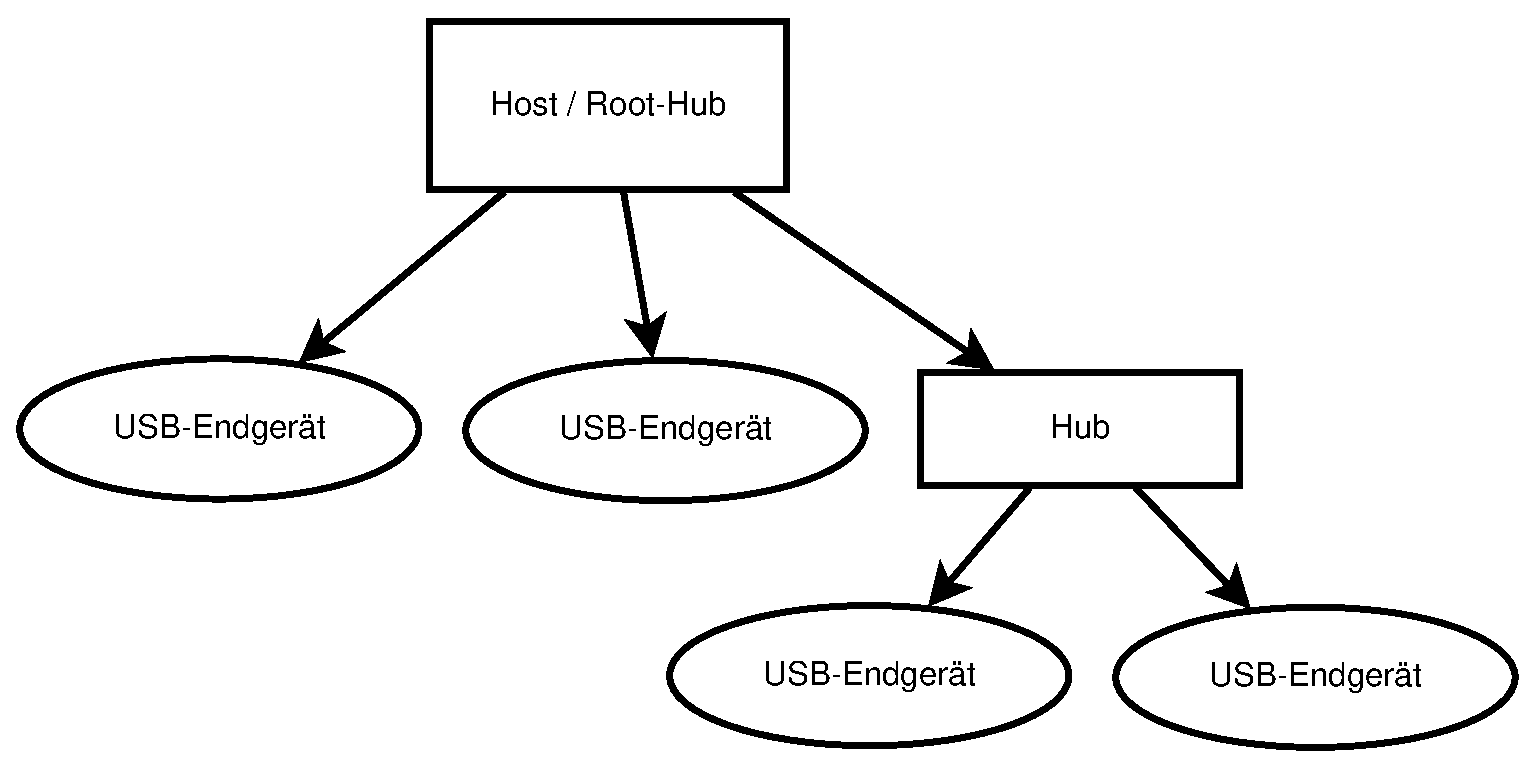
\includegraphics[width=10cm]{images/bus}
\caption{Physikalische Baumstruktur von USB}
\label{bus}
}
\end{figure}

Im logischen Modell bildet der Host den zentralen Mittelpunkt, an dem jedes
Endger�t direkt angeschlossen ist. 
Da es sich bei USB um einen
\glqq{}Single Master Bus\grqq\footnote{\label{foot:1}\glqq{}Single Master Bus\grqq{} bedeutet, es gibt nur einen Teilnehmer auf dem Bus, der jeglichen Datenverkehr initiieren darf.}
handelt, muss der Host jegliche Kommunikation initiieren und steuern.

\begin{figure}[h]
{
\centering
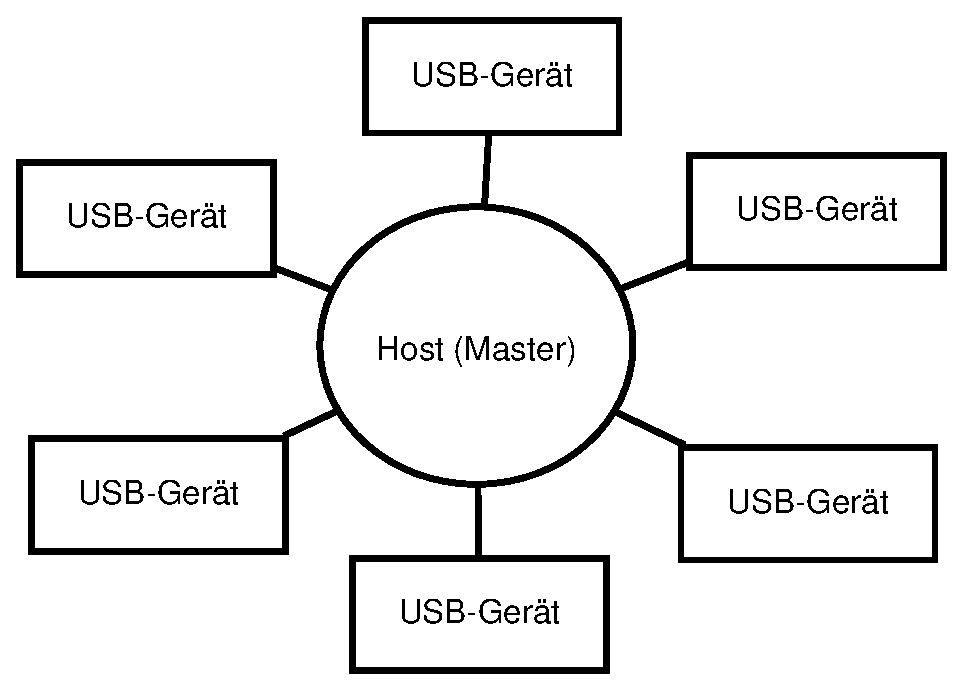
\includegraphics[width=10cm]{images/stern}
\caption{Logische Stern-Architektur von USB}
\label{stern}
}
\end{figure}

Ausgehend von der Topologie werden im n�chsten Abschnitt
die einzelnen Hardwarekomponenten beschrieben.

\section{�bersicht der USB-Komponenten}

\index{USB-Komponenten}

Grundlage f�r den USB-Bus bilden die einzelnen Hardwarekomponenten (siehe Abbildung \ref{komponenten}),
welche im Verbund die Kommunikation erst erm�glichen.
Im Folgenden werden die wichtigsten Komponenten kurz vorgestellt.

\begin{figure}[h]
{
\centering
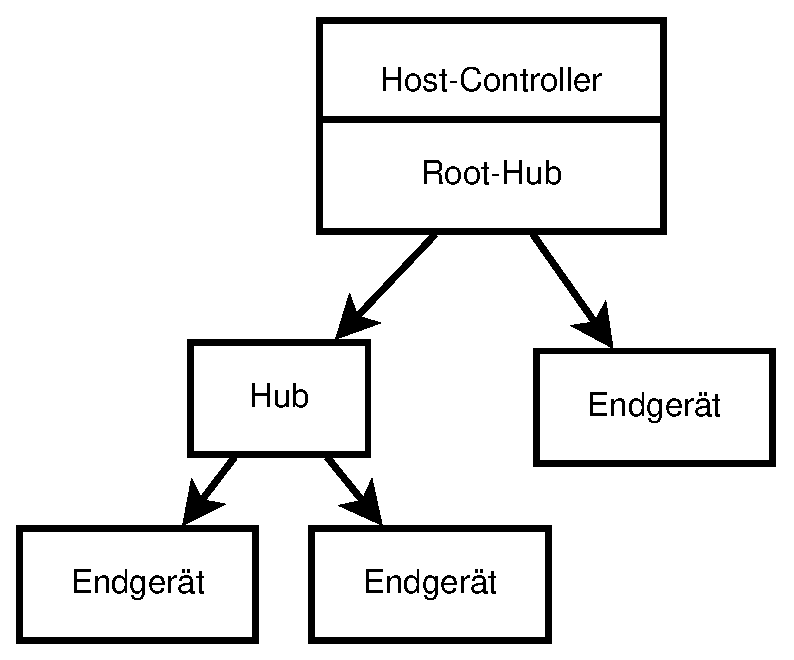
\includegraphics[width=8cm]{images/komponenten}
\caption{�bersicht der USB-Komponenten}
\label{komponenten}
}
\end{figure}

\index{USB-Function}

Der Host-Controller ist f�r die Codierung, �bertragung und dem Empfang der Datenstr�me
von und zu den Endger�ten zust�ndig. 
\newline\newline
Ein USB-Hub ist ein USB-Ger�t genauso wie beispielsweise eine Maus, ein Drucker etc.
Die Aufgabe des Hubs besteht darin, alle ankommenden USB-Signale an zus�tzliche Ports zum Anschluss von weiteren Ger�ten weiterzuleiten.
Hubs k�nnen Strom aus dem Bus beziehen, oder selbst Strom in den USB-Bus einspeisen.
\newline\newline
Der Root-Hub ist ein USB-Hub, der sich direkt hinter dem Host-Controller befindet. 
Der gr��te Unterschied zu einem \glqq{}echten\grqq{} USB-Hub ist der, dass die Status�nderungen an den Ports
des Hubs nicht �ber eine USB-Verbindung abgefragt werden, sondern �ber interne Signale (Interrupts) und Register
signalisiert werden.
\newline\newline
Das Endger�t, welches in der Spezifikation als \glqq{}Function\grqq{} bezeichnet wird,
ist das eigentliche Peripherieger�t und dient meist als Drucker, Scanner, Festspeicher, Kamera, etc.
\newline\newline
Die Aufgaben und die Struktur von USB-Endger�ten werden im n�chsten Abschnitt n�her beschrieben.


%**********************************************************************

\section{Aufgaben und Struktur von USB-Ger�ten}
\index{USB-Ger�t}

Zu den Aufgaben, f�r die ein Ger�t gebaut worden ist, wie z.B. eine Maus f�r die Ermittlung von X-Y Koordinaten,
eine Soundkarte f�r die Ausgabe von Audio-Dateien, etc., muss das Ger�t noch zus�tzliche USB-Verwaltungsarbeiten unterst�tzen.
\newline\newline
\textbf{Erkennen einer Kommunikation: }
Das USB-Ger�t muss erkennen, wenn Daten vom Host angefordert werden.
\newline\newline
\textbf{Antworten auf Standardanfragen: }
�ber die sogenannten Standardanfragen kann ein Betriebssystem, Treiber, Programm, etc.
Informationen direkt beim Ger�t selbst abholen. Mehr dazu in Kapitel \ref{kap:anfragen} auf Seite \pageref{kap:anfragen}. 
\newline\newline
\textbf{Fehlerpr�fung: }
Die ankommenden Datenstr�me m�ssen auf Fehler �berpr�ft und gegebenenfalls 
neu angefordert werden.
\newline\newline
\textbf{Power-Management: }
Ein Ger�t kann sich in verschiedenen Stromverbrauchszust�nden befinden. Um nicht unn�tig
Strom zu verbrauchen, kann zum Beispiel der Host ein Ger�t oder ein Ger�t sich selbst in den Standby-Modus versetzen.
\newline\newline
\textbf{Datenaustausch mit dem Host: }
F�r die Kommunikation mit dem Host m�ssen M�glichkeiten (Pufferspeicher, Status-Register, etc.)
bereitstehen.
\newline\newline
Da diese Aufgaben sehr aufw�ndig sind, gibt es daf�r spezielle USB-Ger�te-Bausteine (engl. \glqq{}USB-Device-Controller\grqq{}).
Mit welchem Anteil der USB-Controller das USB-Protokoll 
per Hardware ausf�hrt, h�ngt ganz vom Hersteller und dessen Zielgruppe
ab. Es gibt eine gro�e Vielfalt an USB-Bausteinen (siehe Tabelle \ref{usb_bausteine}) auf dem Markt.
Grunds�tzlich muss ein USB-Ger�te-Baustein aber mindestens
die folgenden f�nf typischen Teilkomponenten (Abbildung \ref{function}) enthalten.
\newline

\index{SIE}
\index{Transceiver}
\index{FIFO}
\index{Mikrocontroller}
\index{State-Machine}
\index{USBN9604}
\index{AN2131}
\index{MAX34xx}

\begin{figure}[h]
{
\centering
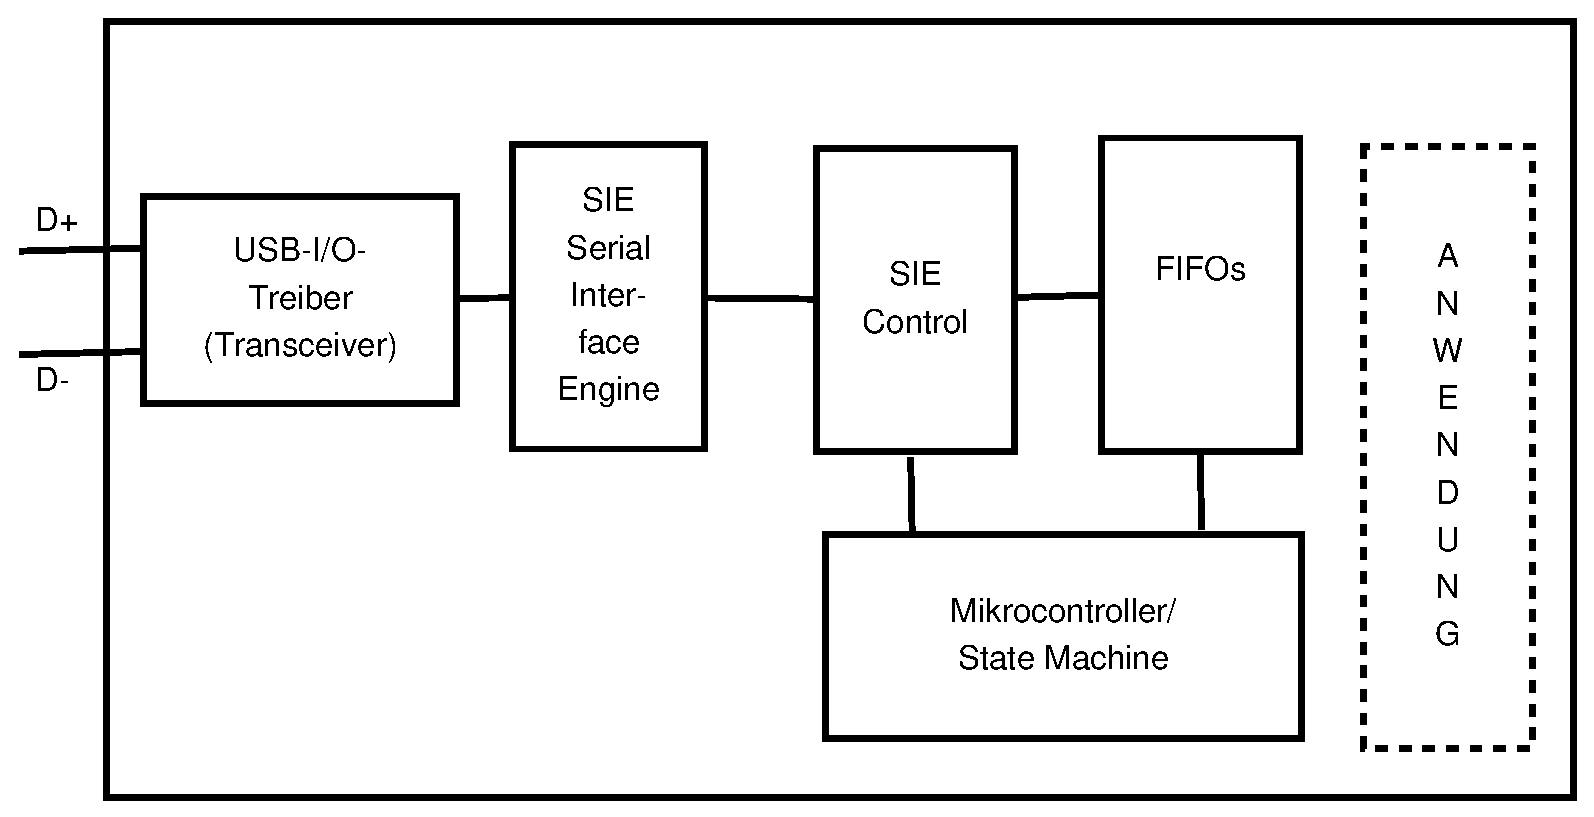
\includegraphics[width=13cm]{images/function}
\caption{Architektur eines USB-Ger�te-Bausteins}
\label{function}
}
\end{figure}

\begin{description}
\item [USB-I/O-Treiber (\glqq{}Transceiver\grqq{}):]
Der USB-I/O-Treiber stellt die physikalische Verbindung zum USB-Bus her. Bis auf ein
paar Ausnahmen muss der USB-I/O-Treiber die seriellen Signale von der \glqq{}SIE\grqq{} (\glqq{}Serial Interface Engine\grqq{})
differentiell �bertragen und empfangene differentielle Signale wieder in ein serielles Signal zur�ckwandeln.
Auf dem Bus werden bestimmte Signale wie EOP (\glqq{}End-Of-Packet\grqq{}), USB-Reset, etc. \cite{kelm2001} nicht differentiell �bertragen.
Diese Zust�nde muss der Treiber erkennen k�nnen. Mehr dazu in Kapitel \ref{kap:signal} auf Seite \pageref{kap:signal}.

\item [Serial Interface Engine (\glqq{}SIE\grqq{}):]
Die SIE ist f�r die Decodierung und Codierung des seriellen Datenstroms zust�ndig. Mehr dazu in Kapitel \ref{kap:signal} auf Seite \pageref{kap:signal}.

\item [SIE/FIFO-Control-Einheit:]
Die SIE/FIFO-Control-Einheit ist ein endlicher Automat der die SIE, die FIFOS und den USB-Treiber entsprechend
den ankommenden Anfragen vom Host ansteuert.

\item [FIFO(s):]
F�r die ankommenden und abgehenden Daten werden FIFO-Speicher als Zwischenpuffer eingesetzt. Sie dienen
meist dem Embedded System als Schnittstelle f�r die Daten�bertragung.

\item [Mikrocontroller oder State-Machine:]
Um die Standardanfragen beantworten und weitere Verwaltungsaufgaben erledigen zu k�nnen, wird ein Mikrocontroller
oder Zustandsautomat ben�tigt.
\end{description}

\begin{table}[h]
\center
\begin{tabular}{|l|c|c|c|c|c|}
\hline
\rowcolor{Gray}[0.9\tabcolsep]
Baustein &  Transceiver & SIE & FIFOs & State Machine & interne CPU\\ \hline
USBN9604 \cite{national} &  x & x & x & x & \\ \hline
AN2131 \cite{cypress} &  x & x & x & x & x\\ \hline
MAX34xx \cite{maxim} &  x &  &  &  & \\ \hline
\end{tabular}
\caption{USB-Bausteine}
\label{usb_bausteine}
\end{table}



Im n�chsten Abschnitt
wird der Datenfluss zwischen dem USB-Host-Controller und dem USB-Ger�te-Baustein beschrieben.


\section{Datenfluss auf dem USB-Bus}

\index{NRZI}
\index{DPLL}
\index{Bitstuffer}

Wie bereits in Kapitel \ref{kap:topologie} erw�hnt, handelt es sich bei USB um einen
\glqq{}Single Master Bus\grqq{}. Das hei�t, dass nur der Host eine Kommunikation
initiieren kann. USB-Ger�te d�rfen ohne Anforderung durch den Host 
nicht senden. 
\newline\newline
W�hrend einer Kommunikation werden auf dem Bus Datenpakete �bertragen.
Mit speziellen Datenpaketen kann eine Adresse f�r den Empf�nger des
folgenden Datenstroms angegeben werden. Die Daten werden dann dennoch im Broadcast-Modus
an alle Teilnehmer im Netz geschickt, und nur das Ger�t, das seine Adresse
im Paket entdeckt, nimmt die Daten an und antwortet.
\newline\newline
In der USB-Spezifikation wird von \glqq{}Downstream\grqq{} gesprochen,
wenn der Host Daten sendet und von \glqq{}Upstream\grqq{},
wenn Daten von einem Ger�t zum Host �bermittelt werden.


\section{Signalleitungen/Datenkodierung} \label{kap:signal}
\index{Signalleitungen}
\index{Datenkodierung}
Ein USB-Kabel (siehe Abbildung \ref{kabel} auf Seite \pageref{kabel}) besteht aus vier Leitungen.
D+ und D-, welche bis auf ein paar Ausnahmen differentiell getrieben werden,
dienen der Daten�bertragung. Vcc und GND sind f�r die Stromversorgung der Endger�te da. \cite{kelm2001}
\begin{figure}[h]
{
\centering
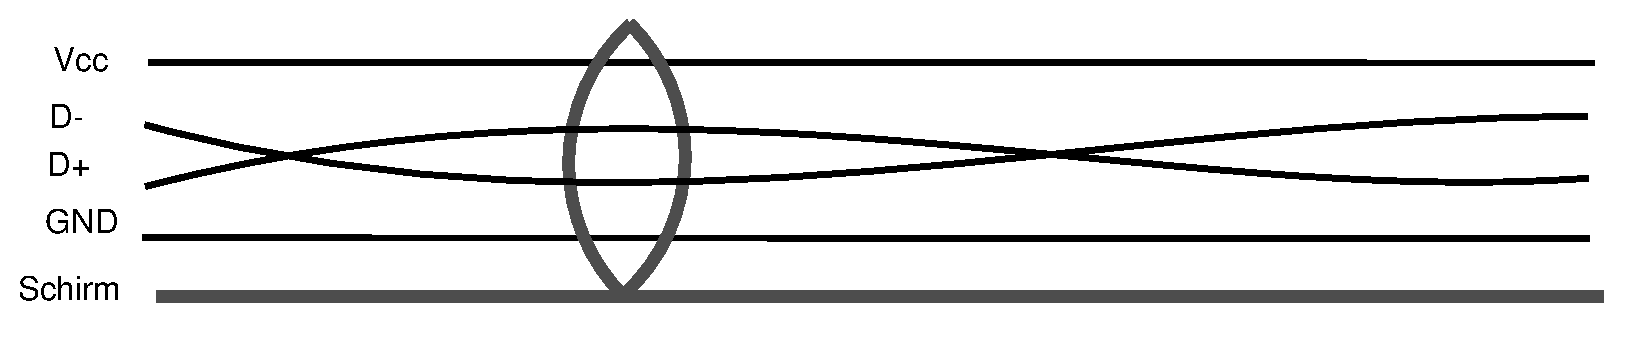
\includegraphics[width=15cm]{images/kabel}
\caption{Querschnitt USB-Kabel}
\label{kabel}
}
\end{figure}
\newline\newline
Auf den Datenleitungen werden ausschlie�lich codierte Daten �bertragen. Das hat zum Ersten den Grund,
dass eine erh�hte Datensicherheit f�r die �bertragung gew�hrleistet ist. Zum Zweiten
kann der Empf�nger den Takt, mit denen die Daten versendet worden sind anhand der empfangenen Daten zur�ckgewinnen.
Technisch l�uft die Codierung wie in Abbildung \ref{nrzi} dargestellt ab.
\newline\newline
Die Daten werden �ber ein Schieberegister serialisiert und anschlie�end
in ein \glqq{}Bitstuffer\grqq{} geschoben. Der \glqq{}Bitstuffer\grqq{} f�gt nach jedem sechsten Bit
eine Null ein. Dies wird f�r den n�chsten Schritt der NRZI-Codierung ben�tigt.
NRZI steht f�r Non-Return-to-Zero-Inverted und ist ein oft verwendetes Codierungsverfahren.
Wird im Eingansdatenstrom eine 0 entdeckt, so findet ein Polarit�tswechsel statt, bei 
einer 1 bleibt der Datenstrom unver�ndert. Der Empf�nger kann sich so mit einer DPLL \cite{dpll}
synchronisieren und den Takt dadurch zur�ckgewinnen.

\begin{figure}[h]
{
\centering
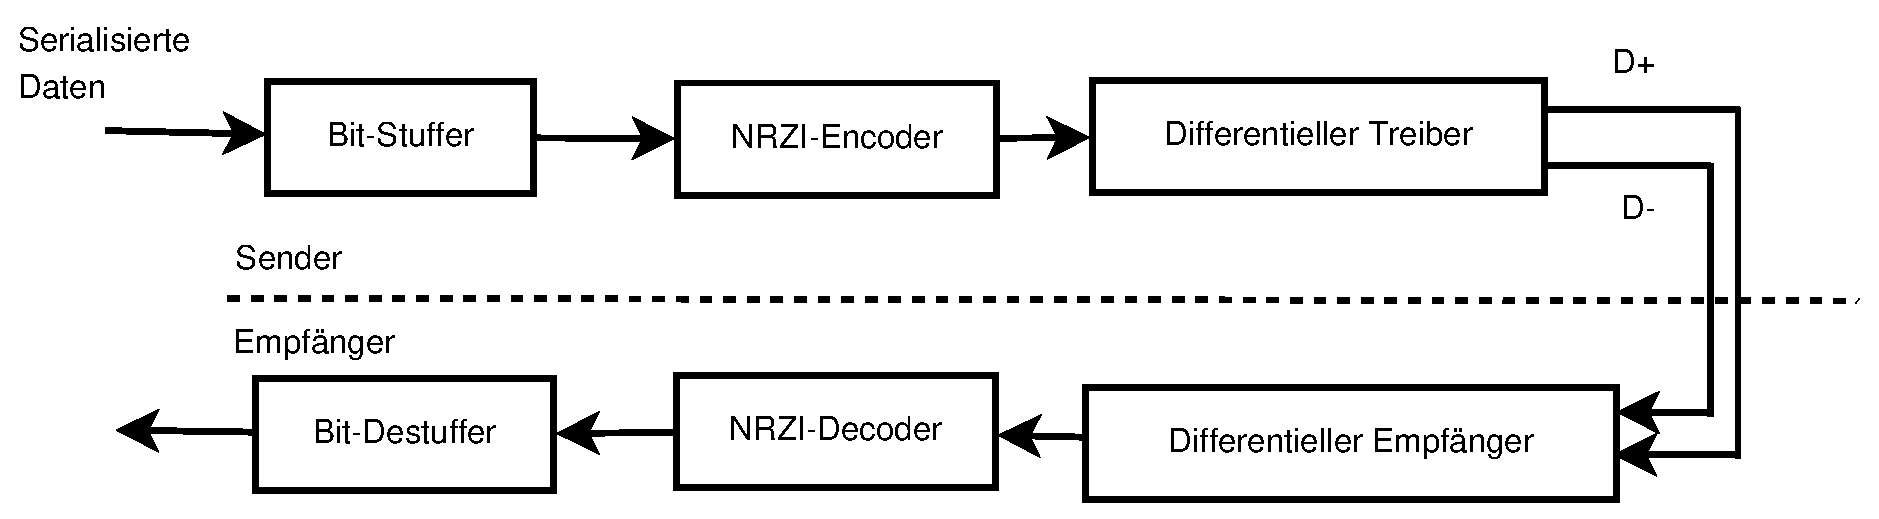
\includegraphics[width=15cm]{images/nrzi}
\caption{Datenfluss der Low-Level-Datencodierung}
\label{nrzi}
}
\end{figure}


\section{Paketformate und Zeitrahmen} \label{kap:pakzei}

Wie bereits erw�hnt, werden auf dem USB-Bus einzelne Pakete (\glqq{}USB-Packets\grqq{}) �bertragen.
In der Tabelle \ref{usb_pid} sind alle verschiedenen Typen von USB-Paketen aufgelistet.

\begin{table}[h]
\center
\begin{tabular}{|l|l|l|}
\hline
\rowcolor{Gray}[0.9\tabcolsep]
PID Name & Gruppe & Beschreibung\\ \hline
SOF & Token-Paket & Framesignalisierung (jede ms) f�r Ger�te\\ \hline
SETUP & Token-Paket & Ank�ndigung einer Standardanfrage\\ \hline
IN & Token-Paket & Host will Daten empfangen\\ \hline
OUT & Token-Paket & Host will Daten senden\\ \hline
DATA0 & Data-Paket & Datenpaket ohne gesetztem Togl-Bit\\ \hline
DATA1 & Data-Paket & Datenpaket mit gesetztem Togl-Bit\\ \hline
ACK & Handshake-Paket & Best�tigungspaket\\ \hline
NAK & Handshake-Paket & �bertragung fehlerhaft - �bertragung wiederholen\\ \hline
STALL & Handshake-Paket & gr�sserer Fehler beim Empfangen - Abbruch\\ \hline
PRE & Special-Paket & k�ndigt Datenempfang bei Low-Speed an\\ \hline
\end{tabular}
\caption{Codierung der USB-Token-Pakete}
\label{usb_pid}
\end{table}

Die Grundstruktur eines USB-Pakets sieht wie in Abbildung \ref{packet} aus.
Jedes Paket beginnt mit
einem 8-Bit langen \textbf{SYNC}-Feld. Dieses
besteht aus 7 Nullen und einer Eins am Ende. Die aufeinander folgenden Nullen
bewirken bei der NRZI-Codierung einen regelm��igen Polarit�tswechsel.
Im Anschluss folgt das 8-Bit breite \textbf{PID}-Feld. Dort steht ein Paket-Typ aus der Tabelle \ref{usb_pid}.
Nach dem PID-Feld folgen abh�ngig vom Paket-Typ paketspezifische Daten. Die \textbf{CRC5}-Pr�fsumme
dient dem Kommunikationspartner zum �berpr�fen der Daten auf Korrektheit, mit \textbf{EOP} (\glqq{}End-of-Paket\grqq{})
wird das Ende des Paketes markiert.

%sync, paket, parameter, crc5, eop
\begin{figure}[h]
{
\centering
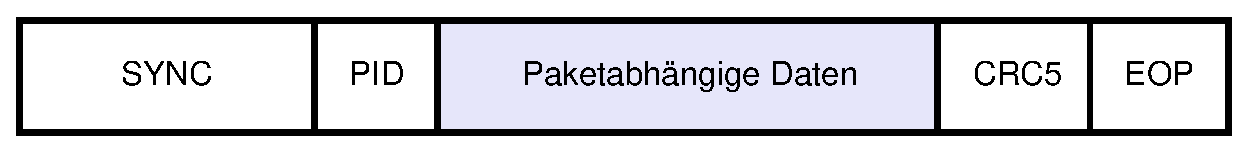
\includegraphics[width=15cm]{images/packet}
\caption{Aufbau der \glqq{}USB-Pakete\grqq{}}
\label{packet}
}
\end{figure}


\index{SNYC}
\index{CRC5}
\index{EOP}
\index{PID}


Der Host versendet jede Millisekunde ein SOF-Paket (\glqq{}Start-of-Frame\grqq{}). Dieses SOF-Paket teilt
den gesamten Bus in einzelne Zeitabschnitte (sogenannte \glqq{}Frames\grqq{}) ein.
Full-Speed und High-Speed Ger�te k�nnen �ber dieses SOF-Paket die Frame-Einteilung erkennen.
Low-Speed Ger�te m�ssen aber wegen ihrer geringen Speicher- und Rechenkapazit�ten vor SOF-Paketen gesch�tzt werden,
da sie sonst ausschlie�lich mit dem Decodieren der SOF-Pakete besch�ftigt w�ren und keine
anderen Pakete mehr annehmen k�nnten. Daher m�ssen Hubs an den Ports, an denen sich Low-Speed Ger�te
befinden, die SOF-Pakete wegfiltern.
Dass Low-Speed Ger�te dennoch die Einteilung der Frames auf dem USB-Bus erkennen, muss
der letzte Hub oder Root-Hub vor dem Ger�t EOP-Signale auf dem Bus erzeugen.
Ein EOP-Signal ist eines von drei speziellen Signalen (siehe Tabelle \ref{speziellsignal}), die nicht differentiell
auf dem USB-Bus �bertragen werden, und ist daher mit viel geringerem Aufwand dekodierbar.
\newline\newline
Zur�ck zu den Aufgaben des SOF-Pakets. Ein SOF-Paket hat noch einen zweiten Nutzen, es dient als Ank�ndigung
f�r weitere Daten-Pakete. Denn nur direkt nach einem SOF-Paket k�nnen Daten-Pakete gesendet werden (siehe Abbildung \ref{zeittakt}).
\begin{figure}[h]
{
\centering
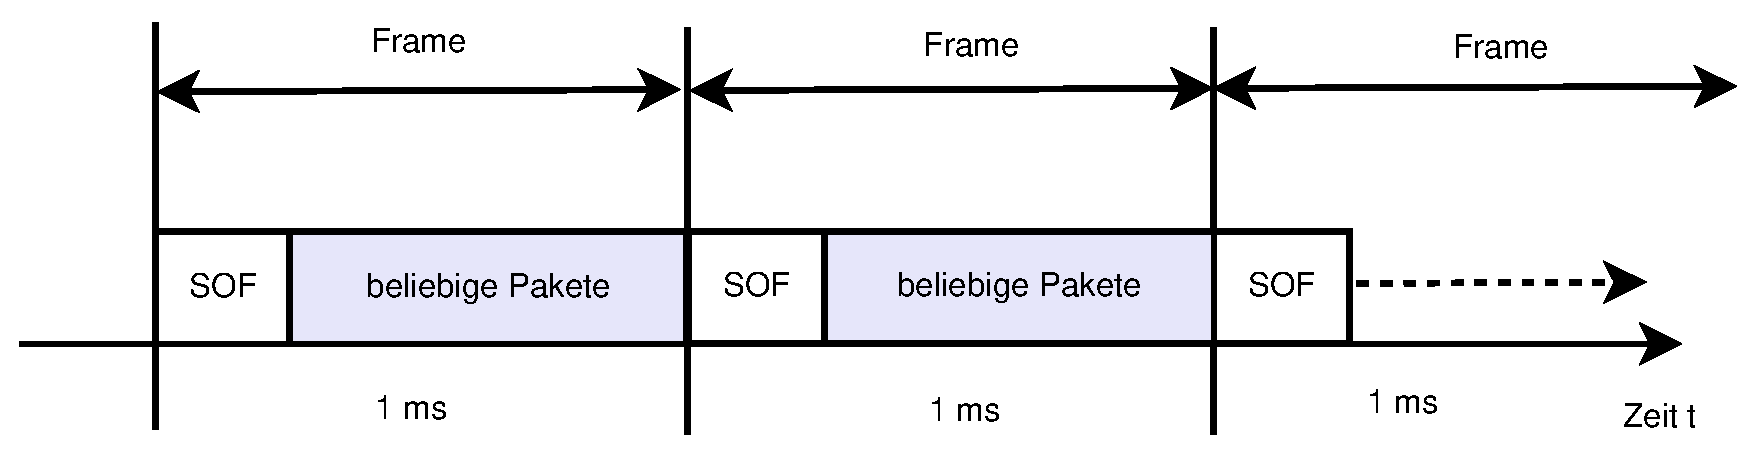
\includegraphics[width=15cm]{images/zeittakt}
\caption{Zeittakt des USB}
\label{zeittakt}
}
\end{figure}
Da Low-Speed Ger�te jedoch keine SOF-Pakete empfangen k�nnen, wird ein Low-Speed Datentransfer mit einem
PRE-Paket (\glqq{}Spezial Token\grqq{}) angek�ndigt.

Im Datenbereich eines SETUP-, IN- oder OUT-Pakets ist eine Ger�teadresse und ein Endpunkt angeben.
Danach k�nnen Daten, verpackt in DATA0- und DATA1-Pakete, f�r das angegebene Ger�t folgen.
Die restlichen Pakete ACK, NAK und STALL dienen zur Flusskontrolle und damit
indirekt zur Umsetzung der verschiedenen Transferarten, die �ber USB angeboten werden.

\index{ACK}
\index{NAK}
\index{STALL}
\index{DATA0,DATA1}

\begin{table}[h]
\center
\begin{tabular}{|l|l|}
\hline
\rowcolor{Gray}[0.9\tabcolsep]
Signal & Beschreibung \\ \hline 
EOP & Signalisiert Ende eines Paketes \\ \hline 
Reset & USB-Ger�t in Reset Zustand zwingen \\ \hline 
Connect & Neues USB-Ger�t wurde angeschlossen\\ \hline
Disconnect & USB-Ger�t wurde entfernt\\ \hline
\end{tabular} \caption{Nicht-differentielle Signale} \label{speziellsignal}
\end{table}

\index{Nicht-differentiellen Signale}

\index{Transferarten}
\index{Control-Transfer}
\index{Bulk-Transfer}
\index{Interrupt-Transfer}
\index{Isochronous-Transfer}

\section{Transferarten}
Um die unterschiedlichen Ger�te und Anwendungen zu unterst�tzen, sind in der USB-Spezifikation
vier verschiedene Transferarten definiert:
\begin{description}
\item[Bulk-Transfer]
Der Bulk-Transfer wird am meisten genutzt. Es k�nnen gro�e und zeitunkritische Datenmengen �bertragen werden. F�r den Bulk-Transfer ist keine feste Bandbreite auf dem Bus reserviert. Er wird nach allen zeitkristischen Transfers durchgef�hrt. Zus�tzlich �berpr�ft dieser Transfer stets die Korrektheit der �bertragenen Daten. 
\item[Interrupt-Transfer]
Diese �bertragungsart darf nicht w�rtlich genommen werden, denn USB ist ein Single Master Bus. Das bedeutet, nur der Master darf jegliche Kommunikation initiieren. Kein Ger�t kann sich beim Master selbst anmelden und ihm mitteilen, dass es Daten �bertragen will. Der Master muss zyklisch alle Ger�te nach neuen Daten abfragen. Im Grunde ist der Interrupt-Transfer nichts anderes als der Bulk-Transfer mit dem Unterschied, dass die Interrupt-Endpunkte eine h�here Priorit�t und daher mehr Bandbreite bekommen. Auf diese Weise kann der Master immer zu dem gew�nschten Zeitpunkt auf das Ger�t zugreifen, selbst dann, wenn gerade viel Datenverkehr auf dem Bus ist.
\item[Isochronous-Transfer]
Mit dem Isochronen Modus k�nnen Daten �bertragen werden, die eine konstante Bandbreite erfordern. Typische Anwendungsbeispiele sind die �bertragung von Audio- oder Videosignalen. Geht hier ein Bit oder Byte verloren, �u�ert sich das im Signal nur mit einem \glqq{}Knacken\grqq{} oder \glqq{}Rauschen\grqq{}. W�rden die Daten aber verz�gert ankommen, w�re die Sprache oder das Bild v�llig verzerrt und daher unbrauchbar.
Es muss ebenso wie beim Interrupt-Transfer das Pollingintervall angegeben werden.
\item[Control-Transfer]
Der Control-Transfer ist an dieser Stelle noch zu erw�hnen. Er wird ausschliesslich beim sogenannten Endpunkt 0 f�r
Standard-, Hersteller-, und Klassenanfragen eingesetzt. F�r andere Endpunkte
kann dieser Transfer nicht verwendet werden. Mehr dazu in Kapitel \ref{kap:anfragen} auf Seite \pageref{kap:anfragen}.
\end{description}

%USB unterscheidet zwischen zwei verschiedenen Pipe-Konzepten: Message-Pipes und Stream-Pipes.
%Daten die �ber eine Message Pipe �bertragen werden, besitzen eine fest vorgegebene Datenstruktur
%durch die USB-Spezifikation. Mit Stream-Pipes k�nnen frei definierte Datenstr�me �bertragen werden.
%Da nur die Anfragen f�r Endpunkt 0 in der USB Spezifikation festgelet sind, ist dies auch der
%einzige Endpunkt der mit dem Message-Pipe Konzept arbeitet. Ebenfalls kann eine Message-Pipe
%nur �ber einen Control-Transfer Endpunkt realisiert werden, welcher wiederrum nur f�r Endpunkt 0 zugelassen ist.
%Daher arbeitet man bei der �bertragung von eigenen Daten immer mit Stream-Pipes die mittels
%Bulk-, Isochronous- oder Interrupt-Transfers realisiert werden.


\section{Endpunkte f�r die Datenkommunikation}

\index{Endpunkte}
\index{Pipe}

Die Datenkommunikation des USB geschieht �ber die sogenannten Endpunkte.
Jedes USB-Ger�t kann bis zu 16 Endpunkte haben.
Physikalisch gesehen ist ein Endpunkt ein FIFO mit einer festgelegten Tiefe, �ber
den Daten gesendet oder empfangen werden k�nnen.
Will ein Anwendungsprogramm oder Treiber Daten empfangen oder senden,
so kann dies �ber eine Anfrage, die die Ger�teadresse, 
den Endpunkt inklusive der gew�nschten Richtung und die Transferart enth�lt, geschehen.
\newline\newline
In modernen USB-Bausteinen, welche f�r den Einsatz in USB-Ger�ten bestimmt sind,
hat man meist ein paar frei definierbare FIFO-Speicher zur Verf�gung. �ber 
vorgesehene Tabellen k�nnen diese eigenen Endpunkten zugeordnet werden.
Dieses Konzept erlaubt die Implementierung von mehreren logisch unabh�ngigen
Ger�ten in einem physikalischen Ger�t. Mehrere Endpunkte k�nnen
in einem Interface geb�ndelt werden, dazu aber mehr in Abschnitt \ref{kap:interfaces}
auf Seite \pageref{kap:interfaces}.
Ist ein Endpunkt komplett mit allen Parametern eingerichtet, dann spricht man von einer \glqq{}Pipe\grqq{}.
\newline\newline
Alle Endpunkte bis auf einen, den sogenannten EP0, k�nnen frei definiert werden.
Der Endpunkt 0 wird vom Host ben�tigt,
um das Ger�t zu konfigurieren. Er ist
der einzige bidirektionale Endpunkt, d.h. �ber ihn k�nnen Daten empfangen und gesendet werden.
\newline\newline
Mit folgenden Parametern kann ein Endpunkt beschrieben werden:
\newline\newline
\textbf{Endpunktadresse:}
Sie definiert die Adresse f�r den gegebenen Endpunkt. In der Endpunktadresse
ist die �bertragungsrichtung ebenfalls durch Bit 7 codiert. Befindet sich eine 1 an Bit 7,
so bedeutet dies, dass der Host von dem Endpunkt lesen kann. Bei einer 0 kann der Endpunkt
Daten vom Host entgegennehmen.
\newline\newline
\textbf{Max. Paketgr��e:}
Die maximale Paketgr��e wird meist durch die Tiefe des dahinter liegenden FIFO-Speichers bestimmt.
F�r den Host bedeutet dies, dass er die Pakete vor dem Transfer in die gegebene Gr��e segmentieren muss.
\newline\newline
\textbf{Transferart:}
Die Transferart, die f�r die �bertragung der Daten genutzt werden soll.
\newline\newline
\textbf{Polling-Intervall:}
Das Polling-Intervall bestimmt bei Endpunkten f�r Interrupt- und Isochronen-Transfer, wie oft 
der Host Daten lesen oder senden muss.
\newline\newline
Die eben genannten Parameter werden in sogenannten Endpunkt-Deskriptoren angegeben. Im n�chsten Kapitel wird
beschrieben, was Deskriptoren sind.

\section{Deskriptoren}

Deskriptoren sind kleine Informationsbl�cke, die im USB-Ger�t gespeichert sind.
Angeordnet sind diese Bl�cke wie in Abbildung \ref{deskriptoren} zu sehen ist.
Betriebssysteme, Treiber oder Programme k�nnen diese Deskriptoren �ber USB 
abfragen. Dadurch ist echtes \glqq{}Plug and Play\grqq{}\footnote{\label{foot:1} engl. \glqq{}anschlie�en und loslegen\grqq{}, bezeichnet
eine Eigenschaft f�r Hardware, wenn diese ohne Treiberinstallation direkt nach dem Anstecken betrieben werden kann.} m�glich.
\begin{figure}[h]
{
\centering
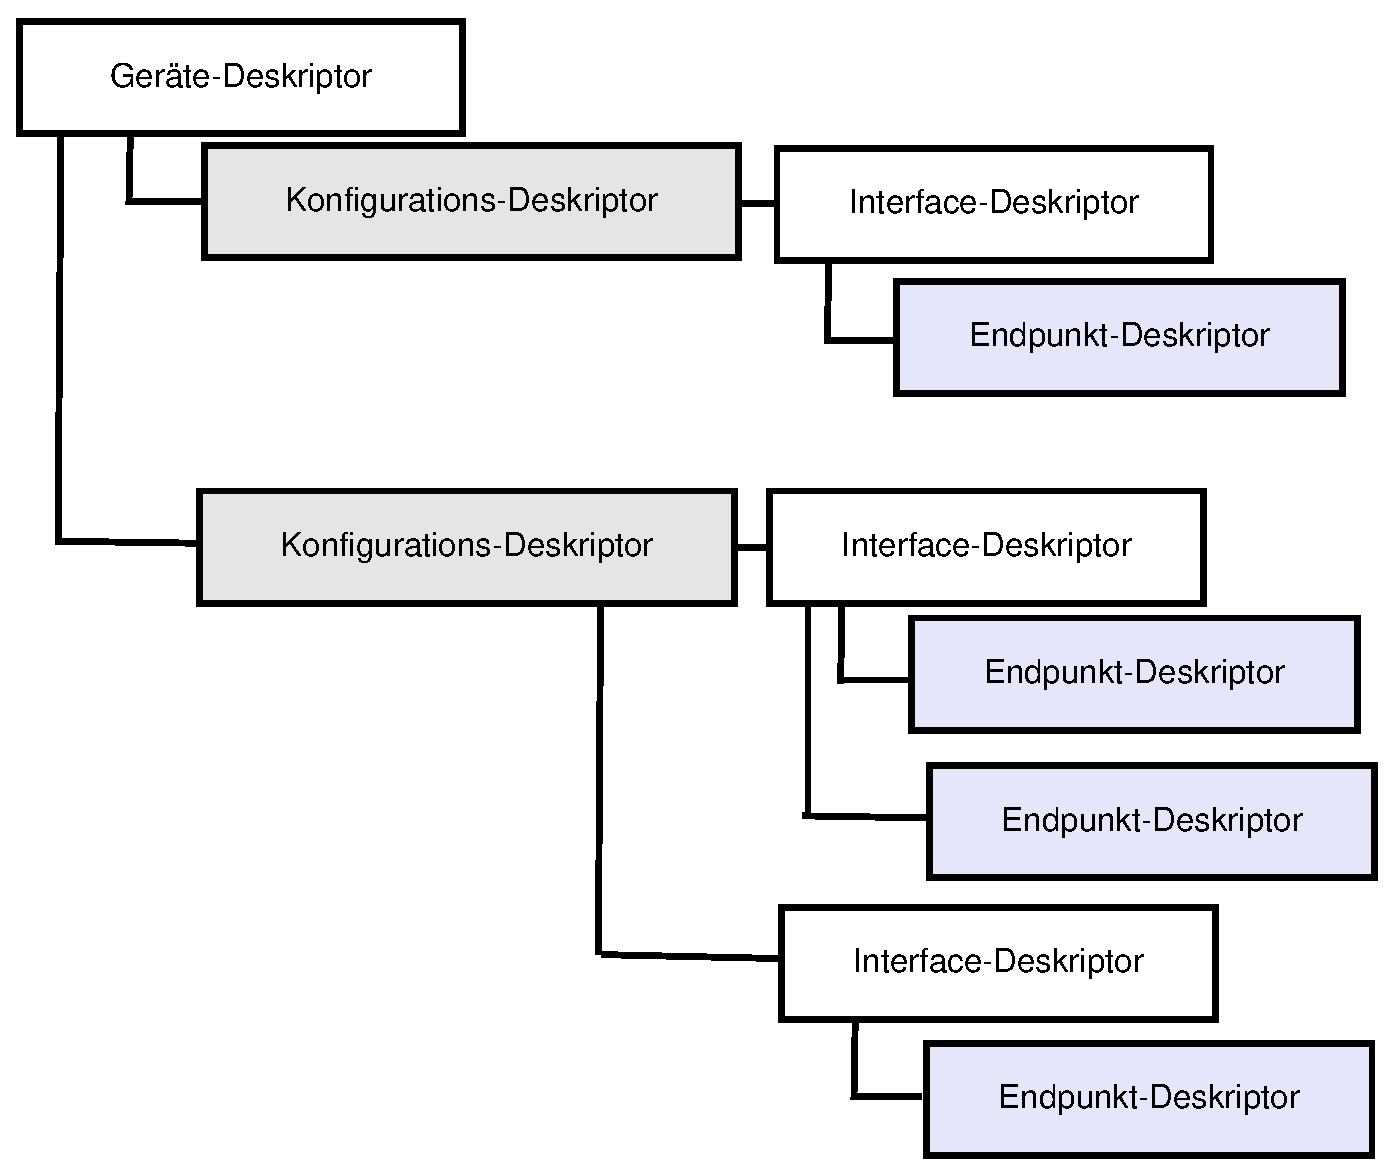
\includegraphics[width=13.5cm]{images/deskriptoren}
\caption{Hierarchie der Standard-Deskriptoren}
\label{deskriptoren}
}
\end{figure}
\index{Deskriptoren}

An der Spitze des Hierarchiebaums der Standard-Deskriptoren steht der Ger�te-Deskriptor (\glqq{}Device-Descriptor\grqq{}).
Im Ger�te-Deskriptor, den es nur einmal pro Ger�t geben kann, befinden sich alle allgemeinen Informationen zu dem Ger�t.
In den Konfigurations-Deskriptoren (\glqq{}Configuration-Descriptor\grqq{}) kann das Stromprofil eingestellt werden.
Die Konfigurations-Deskriptoren k�nnen in einem Ger�t mehrfach vorhanden sein.
Der Vorteil von mehren Konfigurationen
ist, dass �ber USB direkt zwischen den Konfigurationen hin und her geschaltet werden kann. Die Firmware im Ger�t
bekommt diese Umschaltanfrage mit und kann so z.B. den Strom von einem externen Netzteil beziehen oder die Akkus laden,
je nachdem welche Konfiguration aktiviert worden ist.
\newline\newline
Eine Ebene tiefer befinden sich die Interface-Deskriptoren (\glqq{}Interface-Descriptors\grqq{}). Von ihnen kann es ebenfalls mehrere geben,
wobei mindestens einer vorhanden sein muss. Mit einem Interface k�nnen logische Schnittstellen erstellt werden,
da ein Interface immer ein B�ndel von Endpunkten ist. Mehr dazu aber im Kapitel \ref{kap:interfaces}
auf Seite \pageref{kap:interfaces}.
\newline\newline
Auf der letzten Ebene befinden sich die Endpunkt-Deskriptoren (\glqq{}Endpoint-Descriptors\grqq{}). Wie im vorherigen Kapitel erw�hnt,
beschreibt ein Endpunkt alle wichtigen Parameter f�r einen m�glichen Daten�bertragungskanal (\glqq{}Pipe\grqq{}).




\section{Ger�te-Deskriptoren}

\index{Deskriptoren}
\index{Ger�te-Deskriptoren}

Der Ger�te-Deskriptor muss in jedem Ger�t vorhanden sein. Hier sind folgende Parameter definiert:
\newline\newline
\textbf{USB-Version:}
USB-Version, die das Ger�t unterst�tzt (z.B. 1.1).
\newline\newline
\textbf{Klassen- / Subklassen- / Protokoll-Code:}
Das USB-Konsortium hat nicht nur den USB-Bus definiert, sondern gibt auch Beschreibungen f�r Ger�te heraus. So k�nnen Betriebssysteme Standardtreiber anbieten. Mehr zu dieser Technik ist in Kapitel 6 zu finden.
\newline\newline
\textbf{FIFO Tiefe von EP0:}
Tiefe des Endpunkt 0 FIFO in Byte. Bei USB 1.1 ist er meist 8 Byte und bei USB 2.0 64 Byte tief.
\newline\newline
\textbf{Herstellernummer:}
Jeder Hersteller von USB-Ger�ten muss sich beim USB-Forum \cite{usborg} registrieren. 
Daf�r bekommt er eine eindeutige Nummer, die f�r die Treibersuche des Betriebssystems von Bedeutung ist.
\newline\newline
\textbf{Produktnummer:}
Die Produktnummer wird (wenn sie definiert ist) vom Treiber verwendet, um das Ger�t eindeutig zu identifizieren. 
\newline\newline
\textbf{Versionsnummer:}
Versionsnummer f�r das Ger�t.
\newline\newline
\textbf{String Index f�r Hersteller-, Produkt- und Seriennummer:}
Im Ger�tedeskriptor wird nicht direkt der Name f�r Hersteller-, Produkt- oder Seriennummer gespeichert, sondern nur ein Index f�r einen sogenannten String-Deskriptor. 
\newline\newline
\textbf{Anzahl der Konfigurationen:}
Die Anzahl der vorhandenen Konfigurationen f�r das Ger�t. Ein Ger�t muss mindestens eine Konfiguration haben.

\section{Powermanagement mit Konfigurationen}
Ebenso wie mehrere Interfaces kann ein Ger�t mehrere Konfigurationen haben. Hier geht es um die elektrischen Eigenschaften. Bei USB k�nnen die Ger�te direkt �ber das USB-Kabel mit Strom versorgt werden. So kann man von einem Bus maximal 500 mA bei 5 V Spannung beziehen. Bevor ein Ger�t den Strom nutzen kann, muss es beim Master anfragen, ob noch gen�gend freie Kapazit�ten vorhanden sind.

In einer Konfiguration m�ssen folgende Parameter definiert sein:

\begin{enumerate}
\item Stromaufnahme in 2 mA Einheiten.
\item Attribute (z.B. Bus-Powered, Remote-Wakeup-Support).
\item Anzahl der Interfaces unter dieser Konfiguration.
\end{enumerate}

\section{Interfaces zum B�ndeln von Endpunkten} \label{kap:interfaces}
Interfaces sind zum B�ndeln von Endpunkten da. 
Ein Ger�t kann mehrere Interfaces anbieten. So ist es m�glich, dass eine Soundkarte ein Interface f�r den Mono- und eines f�r den Stereobetrieb anbietet. Das Interface f�r den Monobetrieb hat einen Endpunkt f�r die Steuerkommandos und einen weiteren f�r die Daten, die �ber einen Lautsprecher ausgegeben werden. Das Interface f�r den Stereobetrieb hat ebenfalls einen Endpunkt f�r Steuerkommandos, jedoch zwei f�r die Signalausgabe (linker und rechter Kanal). Die Software auf dem PC kann jederzeit zwischen den Interfaces hin- und herschalten. 
\newline\newline
Im gleichen Zug mit Interfaces liest man oft den Begriff \glqq{}Alternate-Interface\grqq{}. Dieses Interface kann parallel zu einem anderen Interface definiert werden. Definiert man ein normales Interface, so gibt man dort die Endpunkte an, die zu ihm geh�ren. Entsprechend der FIFO-Gr�sse eines Endpunktes wird die entsprechende Bandbreite auf dem USB-Bus reserviert.
Die Bandbreite w�re auf diese Weise sehr schnell aufgebraucht, auch ohne dass Kommunikation auf dem Bus stattfindet. W�rde man jedoch die ben�tigte Bandbreite immer nur kurz vor dem Senden oder Empfangen reservieren, k�nnte man viel mehr Ger�te �ber einen Bus bedienen. Daher wurde das Alternate-Interface erfunden. Zu jedem Interface kann es also ein alternatives Interface geben. Die Endpunktstruktur sollte genauso aussehen, wie die vom normalen Interface. Der einzige Unterschied ist der, dass �berall als FIFO-Gr�sse 0 Byte angegeben ist. Gibt es nun ein Alternate-Interface, aktiviert das Betriebsystem beim Einstecken erst dieses, und nimmt so nicht voreilig anderen USB-Ger�ten die Bandbreite weg. Kurz vor dem Senden und Empfangen wird dann auf das eigentliche Interface gewechselt. 



\section{Standard-, Hersteller- und Klassenanfrage} \label{kap:anfragen}
\index{Vendor-Requests}
\index{Class-Requests}
\index{Default-Requests}
\index{Herstelleranfragen}
\index{Standardanfragen}
\index{Klassenanfragen}
In vorherigen Kapitel wurde bereits erw�hnt, dass die Deskriptoren eines USB-Ger�tes jederzeit abgefragt werden k�nnen.
Daf�r wird der Endpunkt 0 und der darauf basierende Control-Transfer ben�tigt. In der USB-Spezifikation
wurden Standardanfragen, die jedes USB-Ger�t beantworten muss, definiert. Abbildung \ref{abfrage} soll
veranschaulichen, wie solch eine Abfrage aussieht. 

\begin{figure}[h]
{
\centering
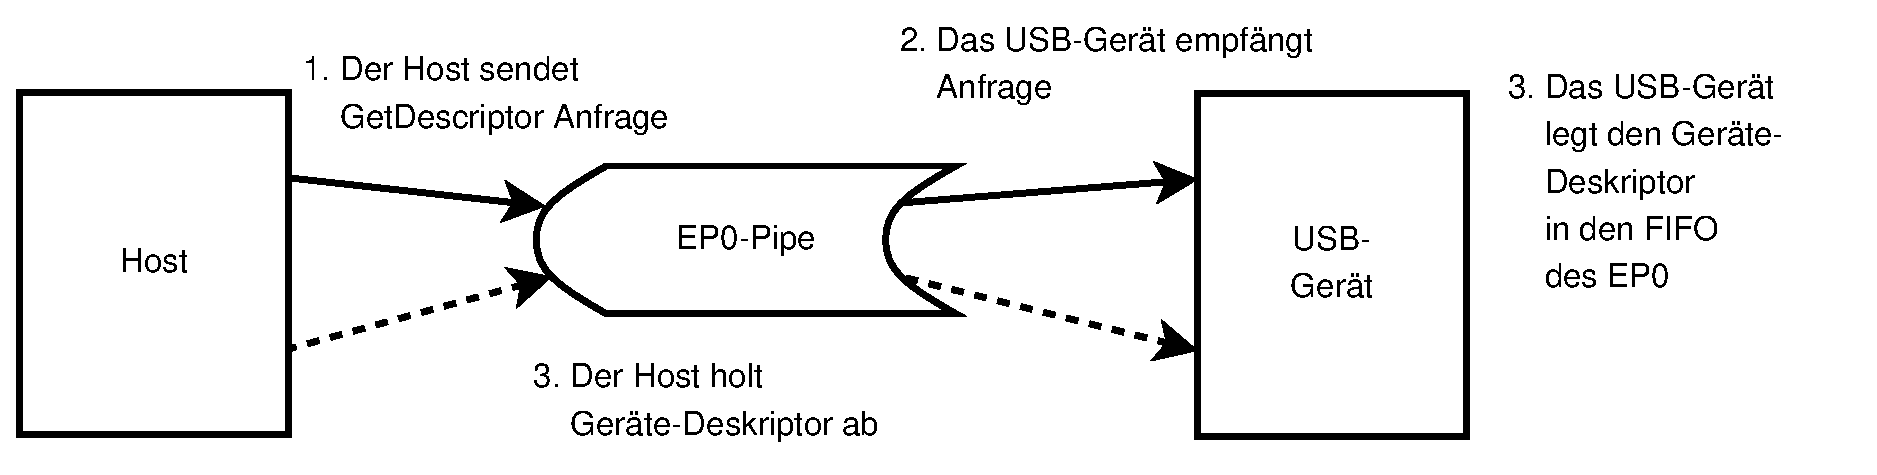
\includegraphics[width=13.5cm]{images/abfrage}
\caption{Abfrage Ger�te-Deskriptor}
\label{abfrage}
}
\end{figure}

\begin{enumerate}
\item Der Host sendet �ber den Endpunkt 0 die Anfrage f�r den Ger�te-Deskriptor an das USB-Ger�t.
\item Das USB-Ger�t empf�ngt die Anfrage und wertet diese aus.
\item Das USB-Ger�t legt den Ger�te-Deskriptor in den FIFO des Endpunktes 0.
\item Der USB-Host holt den Ger�te-Deskriptor �ber den Endpunkt 0 vom FIFO ab.
\end{enumerate}

Zwischen den einzelnen Schritten werden zus�tzlich Pakete f�r die Flusskontrolle 
versendet und ausgewertet. So best�tigt das USB-Ger�t immer mit einem ACK-Paket,
dass eine Anfrage erfolgreich entgegengenommen wurde. Gab es St�rungen beim Empfang,
so kann das USB-Ger�t das letzte Paket nochmals mit einem NAK-Paket neu anfordern.
\newline\newline
Die \glqq{}GetDescriptor\grqq{}-Anfrage ist nur eine von insgesamt elf verschiedenen Anfragen,
die ein USB-Ger�t beantworten k�nnen muss. Eine Auflistung ist in Tabelle \ref{usb_desc} gegeben.

\begin{table}[h]
\center
\begin{tabular}{|l|l|}
\hline
\rowcolor{Gray}[0.9\tabcolsep]
Anfrage & Beschreibung \\ \hline 
GetStatus & Abfrage des Stromverbrauchszustands \\ \hline 
ClearFeature & Vordefinierte Eigenschaften ausschalten \\ \hline 
SetFeature & Eigenschaft einschalten (z.B.Ger�t aus dem Standby wecken) \\ \hline 
SetAddress & Adresse zuweisen \\ \hline 
GetDescriptor & Deskriptor anfordern \\ \hline 
SetDescriptor & �ndern von Deskriptoren (z.B. Seriennummer) \\ \hline 
GetConfiguration & Aktuelle Konfiguration abfragen \\ \hline 
SetConfiguration & Auf eine andere Konfiguration wechseln \\ \hline 
GetInterface & Aktives \glqq{}Alternate-Inferface\grqq{} detektieren \\ \hline 
SetInterface & \glqq{}Alternate-Interface\grqq{} f�r ein Interface aktivieren \\ \hline 
SynchFrame & Zum Synchronisieren von isochronen Endpunkten\\ \hline 
\end{tabular} \caption{Die Standardanfragen} \label{usb_desc}
\end{table}

Einige dieser Anfragen werden bei der Enumeration\footnote{\label{foot:1} Aktivierung eines
neu erkannten Ger�tes am USB-Bus} ben�tigt. Wie die Enumeration genau aussieht,
wird im folgenden Kapitel beschrieben.
\newline\newline
\large{\textbf{Hersteller- und Klassenanfragen}}\normalsize
\newline\newline
Zus�tzlich zu den Standardanfragen k�nnen Hersteller- und Klassenanfragen �ber
die Endpunkt-0-Pipe �bertragen werden. Sie dienen genauso
wie die Standardanfragen der Konfiguration des Ger�tes.

\section{Enumeration}

Bevor eine Anwendung mit einem USB-Ger�t kommunizieren kann,
muss der Host erst feststellen, um was f�r ein Ger�t es sich handelt, und welcher Treiber
gegebenenfalls geladen werden muss. Dies geschieht �ber die Standardanfragen,
die der Endpunkt 0 unterst�tzen muss. W�hrend dieses Vorgangs, der als Enumeration
bezeichnet wird, durchl�uft das USB-Ger�t vier von sechs m�glichen Zust�nden (siehe Abbildung \ref{devzustand}): Powered, Default,
Address und Configured. Die anderen beiden Zust�nde Attached und Suspended werden w�hrend
der Enumeration nicht durchlaufen. Der �bergang von einem Zustand in den anderen
kann nur durch bestimmte Ereignisse ausgel�st werden. 
\newline\newline

\begin{figure}[h]
{
\centering
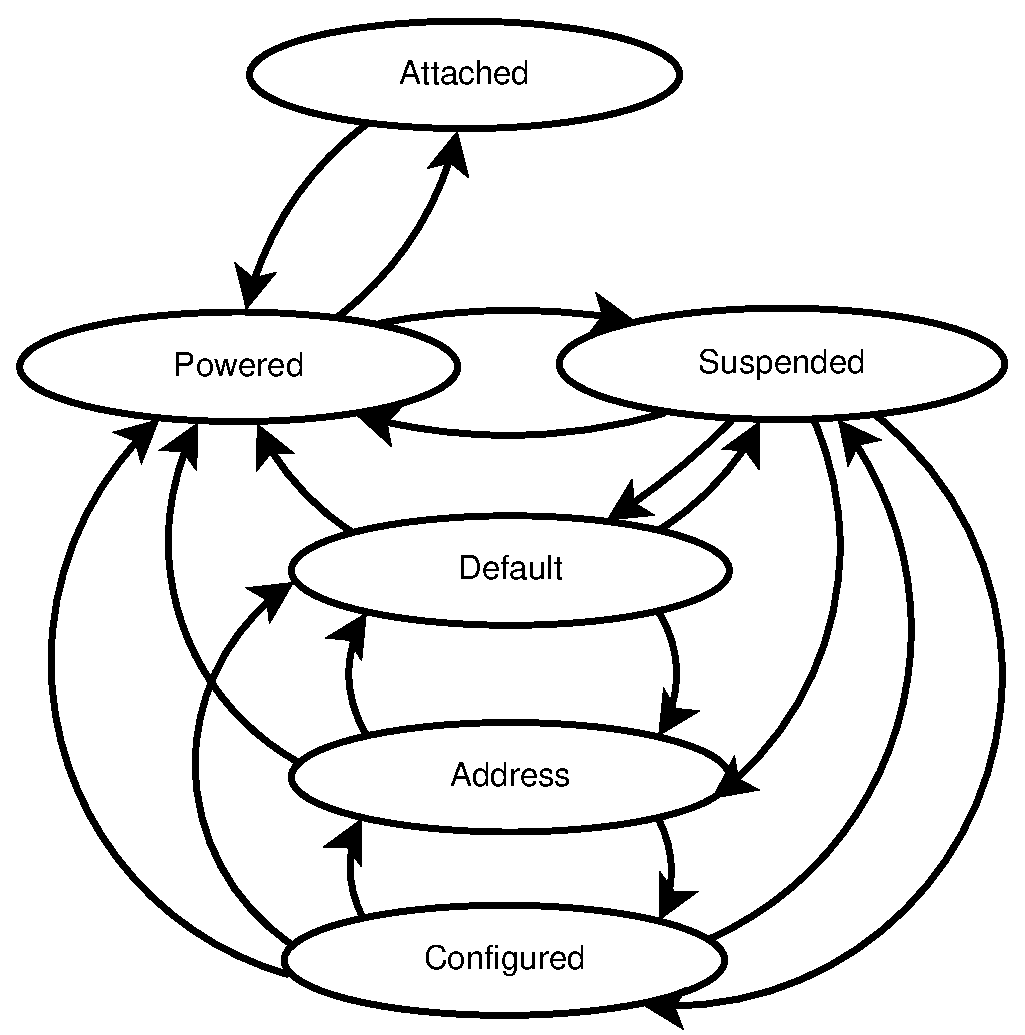
\includegraphics[width=8cm]{images/devzustand}
\caption{Ger�tezustandsdiagramm}
\label{devzustand}
}
\end{figure}
\index{Enmumerierung}

\textbf{1. USB-Ger�t wird angesteckt (Attached):}
Das USB-Ger�t wird angesteckt oder der Strom wird beim Systemstart eingeschaltet.
\newline\newline
\textbf{2. Ger�t wird erkannt (Powered, Suspended):}
Der Root-Hub oder ein anderer Hub meldet dem Host das neu gefundene Ger�t.
\newline\newline
\textbf{3. Reset des Ger�ts wird vorgenommen (Default):}
Der Host veranlasst entweder �ber den Root-Hub oder den Hub einen Reset des neuen Ger�ts. Durch
diesen Reset wird das Ger�t gezwungen, die Adresse 0 anzunehmen. Dadurch
kann der Host nach dem Reset das Ger�t �ber die Adresse 0 ansprechen.
\newline\newline
\textbf{4. Ermitteln der maximalen Paketgr��e f�r die Standard-Pipe (Default):}
Um die Gr��e des Endpunkt 0 herauszubekommen, sendet der Host eine \glqq{}GetDescriptor\grqq{}-Anfrage
f�r den Ger�te-Deskriptor an das Ger�t. Das USB-Ger�t antwortet mit den ersten acht Byte 
des Ger�te-Deskriptors. Da das achte Byte die Gr��e des Endpunkt 0 FIFOs enth�lt, stoppt
der Host die Antwort des USB-Ger�tes.
\newline\newline
\textbf{5. Ger�t bekommt eine Adresse zugewiesen (Address):}
Da der USB-Host nun die genaue Paketgr��e f�r den Enpunkt 0 kennt, kann
er die Pakete in der richtigen Gr��e an das USB-Ger�t schicken. Die erste
Anfrage ist \glqq{}SetAddress\grqq{}, mit der dem Ger�t eine endg�ltige Adresse zugewiesen wird.
\newline\newline
\textbf{6. Informationen vom Ger�t werden abgefragt (Address):}
Anschlie�end fragt der Host �ber die neue Adresse alle Ger�teinformationen ab.
\newline\newline
%\item[Treiber werden geladen:]
%Anhand der Ger�teinformationen kann das Betriebssystem einen geeigneten Treiber laden.
\textbf{7. Konfiguration wird gew�hlt (Configured):}
Um mit dem Ger�t Daten austauschen zu k�nnen, muss eine Konfiguration aktiviert werden.
\newline\newline

Mit dem Beispiel aus Abbildung \ref{beispiel} soll verdeutlicht werden, wie die Deskriptoren zusammenh�ngen und angeordnet sein m�ssen.
\begin{figure}[h]
{
\centering

\includegraphics[width=15cm]{images/beispiel}
\caption{Beispiel-Deskriptoren}
\label{beispiel}
}
\end{figure}



	
\chapter{Die Komponenten und ihre Aufgaben im USB-Host-Stack}


Ein guter Entwurf der Struktur des USB-Stacks ist eine wichtige Basis f�r
die Stabilit�t und die Leistungsf�higkeit der gesamten Software. In diesem Kapitel werden die wichtigsten 
Komponenten des USB-Stacks und deren Aufgaben beschrieben.
Es wird ausschlie�lich auf die theoretischen Hintergr�nde
eingegangen und erst sp�ter im n�chsten Kapitel wird die Struktur und
die Umsetzung in Quelltext erkl�rt.

\section{Host-Stack}

Der USB-Stack wurde, soweit es m�glich und machbar war
nach der USB-Spezifikation implementiert. 
Da die USB-Spezifikation f�r einen Softwarestack auf einem 
PC geschrieben wurde, musste bei der Realisierung des Host-Stack f�r 
ein Embedded System Nutzen und Aufwand in Einklang gebracht werden.

\subsection{�bersicht des Protokoll-Stacks}

\index{Protokoll-Stack}

Der USB-Stack beinhaltet vom Hardwaretreiber bis hin zu den verschiedenen Ger�tetreibern alle Softwarekomponenten (siehe Abbildung \ref{struktur}), 
die f�r den USB-Betrieb n�tig sind.
F�r die
einzelnen Aufgaben wurden jeweils gesonderte Module entwickelt, welche ihre Dienste
�ber definierte Schnittstellen anbieten. 

\begin{figure}[h]
{
\centering
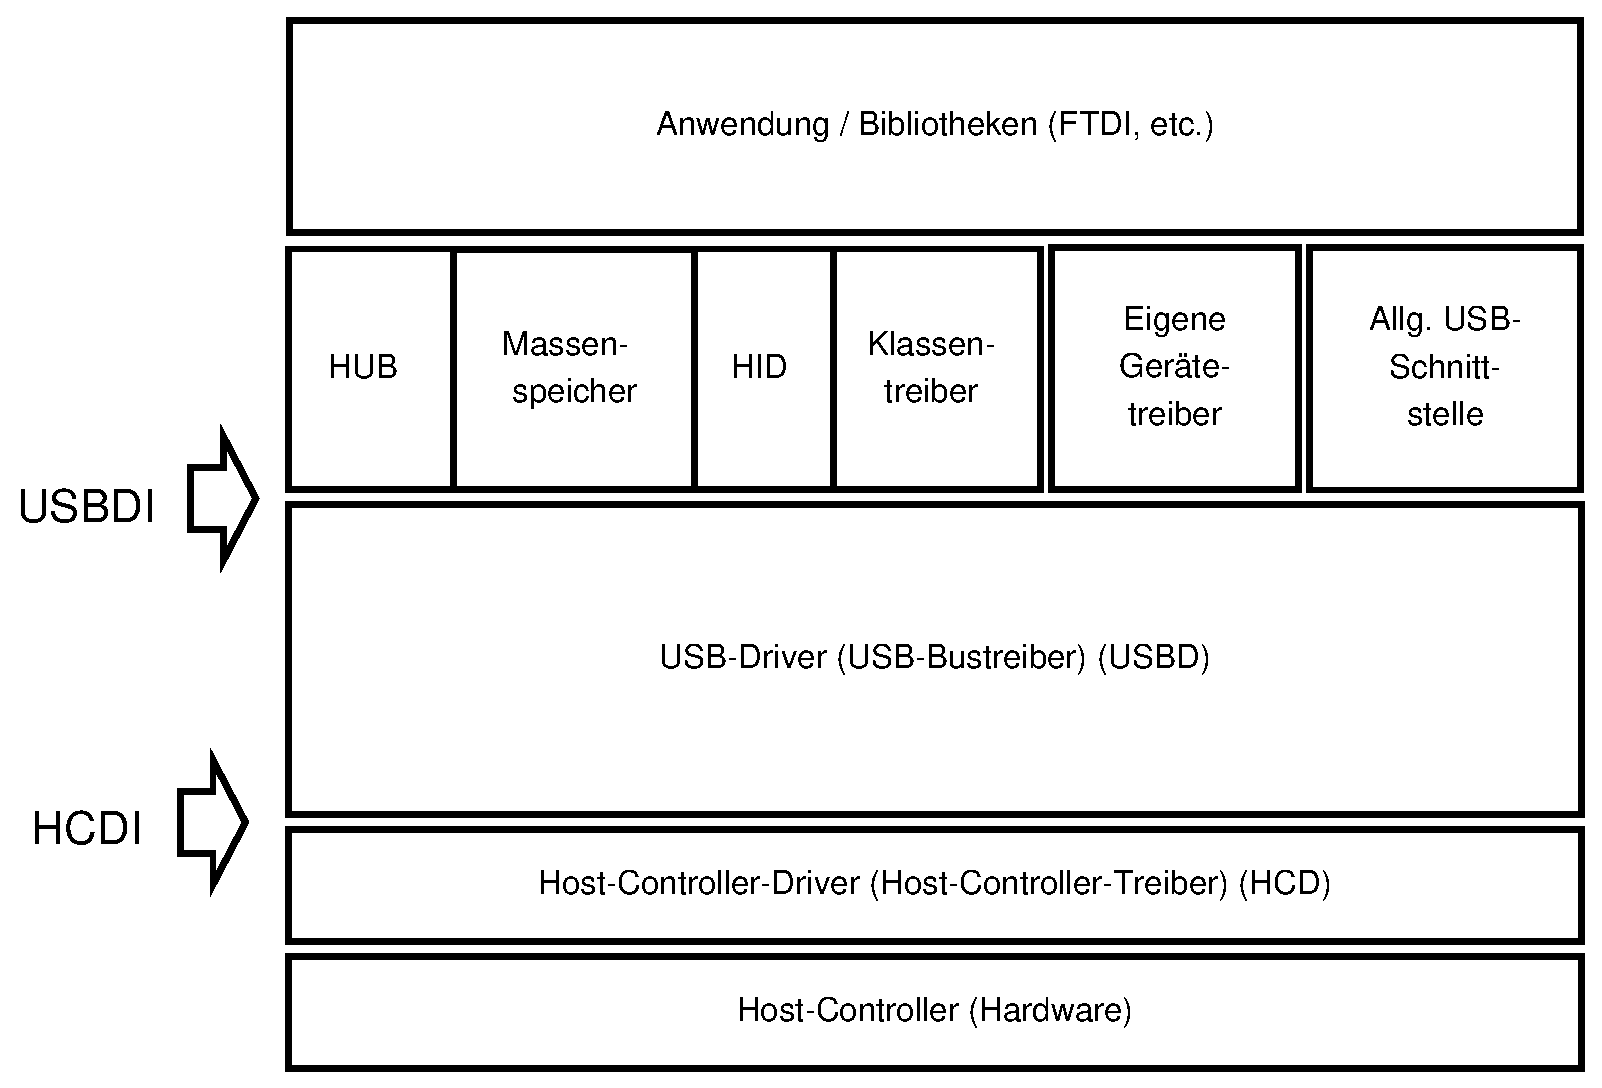
\includegraphics[width=11.5cm]{images/struktur}
\caption{Architektur des USB-Stacks}
\label{struktur}
}
\end{figure}

\index{Host-Controller}
\index{Host-Controller-Treiber}
\index{USB-Bustreiber}
\index{Host-Controller-Driver-Interface}
\index{USB-Bustreiber-Interface}

Auf diese Weise kann der Stack flexibel erweitert und in Anwendungen
integriert werden. Unterst�tzt der Stack eine bestimmte Aufgabe oder einen gewissen
Baustein nicht, so muss nur die fehlende Funktionalit�t nachprogrammiert und in 
das bestehende System eingebunden werden. 
\newline\newline
Im folgenden Abschnitt werden die wichtigen Bezeichnungen aus der Abbildung \ref{struktur} 
zur besseren �bersicht durch Fettdruck hervorgehoben.
\newline\newline
Der Softwarestack bietet f�r die Daten�bertragung verschiedene Ebenen an, die die Nachrichten �ber
USB durchlaufen m�ssen. Die unterste Ebene beinhaltet die physikalische Verbindung auf den USB-Bus.
Realisiert wird diese mittels des \textbf{Host-Controllers (Hardware)}. F�r den Host-Controller
wird ein Treiber ben�tigt, der die Kommunikation mit dem Baustein erm�glicht. Dies ist bereits die Aufgabe
der zweiten Ebene des \textbf{Host-Controller-Treibers (HCD)}.
Die notwendige Verbindung vom Host-Controller-Treiber zum \textbf{USB-Bustreiber (USBD)}, der eine Ebene
�ber dem HCD liegt, wird \textbf{Host-Controller-Driver-Interface (HCDI)} genannt.
Das HCDI bietet f�r den USB-Bustreiber allgemeine Funktionen f�r die Kommunikation mit einem beliebigen Host-Controller an.
Soll ein neuer Host-Controller in den Stack integriert werden, 
so m�ssen nur die Funktionen des HCDI f�r den neuen Controller programmiert werden.
\newline\newline
Auf der dritten Ebene befindet sich der USB-Bustreiber. Er bildet die zentrale Verwaltungs- und
Steuerungskomponente. In dieser Ebene werden Ger�te bzw. Treiber verwaltet und Datenstr�me verteilt.
Der USB-Bustreiber bietet seine Funktionen (Datenkommunikation, Ger�te- und Treiberverwaltung) 
�ber das \textbf{USB-Bustreiber-Interface (USBDI)}
den dar�ber liegenden Schichten an. Die Ger�te bzw. die Treiber aus den dar�ber liegenden Schichten k�nnen nie direkt mit
dem Host-Controller kommunizieren, sondern m�ssen immer �ber das USBDI gehen.
\newline\newline
Zu guter Letzt k�nnen die \textbf{Anwendungen} die Dienste �ber die entsprechenden
Treiberschnittstellen der \textbf{Ger�te- und Klassentreiber} nutzen.

\subsection{Datenfluss einer USB-Nachricht}
\index{USB-Nachricht}
\index{USB-Pakete}
\index{Transfer-Deskriptoren}
\index{I/O-Request-Paket}

In diesem Abschnitt wird der Verlauf einer USB-Nachricht
im USB-Stack betrachtet. 
\newline\newline
Eine USB-Nachricht ist eine Anfrage einer Anwendung bzw. eines Treibers, die �ber
das USBDI \footnote{\label{foot:usbdi} \glqq{}USB-Bustreiber-Interface\grqq{} enth�lt alle Funktionen f�r den Datenaustausch mit Ger�ten.} 
abgesendet werden kann. Eine USB-Nachricht enth�lt entweder Daten f�r
das Ger�t, oder eine Anfrage f�r Daten vom Ger�t. 
Die Nachricht muss immer mit der entsprechenden Transferfunktion aus dem USBDI mit
der Transferart des Zielendpunktes �bertragen werden.
\newline\newline
Eine USB-Nachricht sieht, unabh�ngig von der Transferart, strukturell
immer gleich aus. Es muss die Ger�teadresse, der Endpunkt, die Transferart, die �bertragungsrichtung,
eine Anzahl und ein Puffer f�r die zu sendenden oder zu empfangenden Daten angegeben werden.
In der USB-Spezifikation wird diese Datenstruktur \glqq{}I/O-Request-Packet (IRP)\grqq{} genannt.
M�chte eine Anwendung oder ein Treiber Daten versenden, so muss solch eine Anfrage erzeugt
und dem USB-Bustreiber �bergeben werden. 
\newline\newline
Wie bereits erw�hnt, werden auf dem USB-Bus aber nur USB-Pakete �bertragen. Dies bedeutet
f�r den Host, dass er die vorliegende USB-Nachricht in einzelne Pakete aufteilen muss (siehe Abbildung \ref{irp}).
Abh�ngig von der Transferart werden SETUP-, IN-, OUT-, DATA0- oder DATA1-Pakete generiert. Diese einzelnen
Pakete werden in einer Datenstruktur, die Transfer-Deskriptor genannt wird, gepackt. Ein Transfer-Deskriptor
enth�lt die kleinste USB-Einheit, die mit einem Host-Controller �bertragen werden kann - ein USB-Paket.
\newline\newline

\begin{figure}[h]
{
\centering
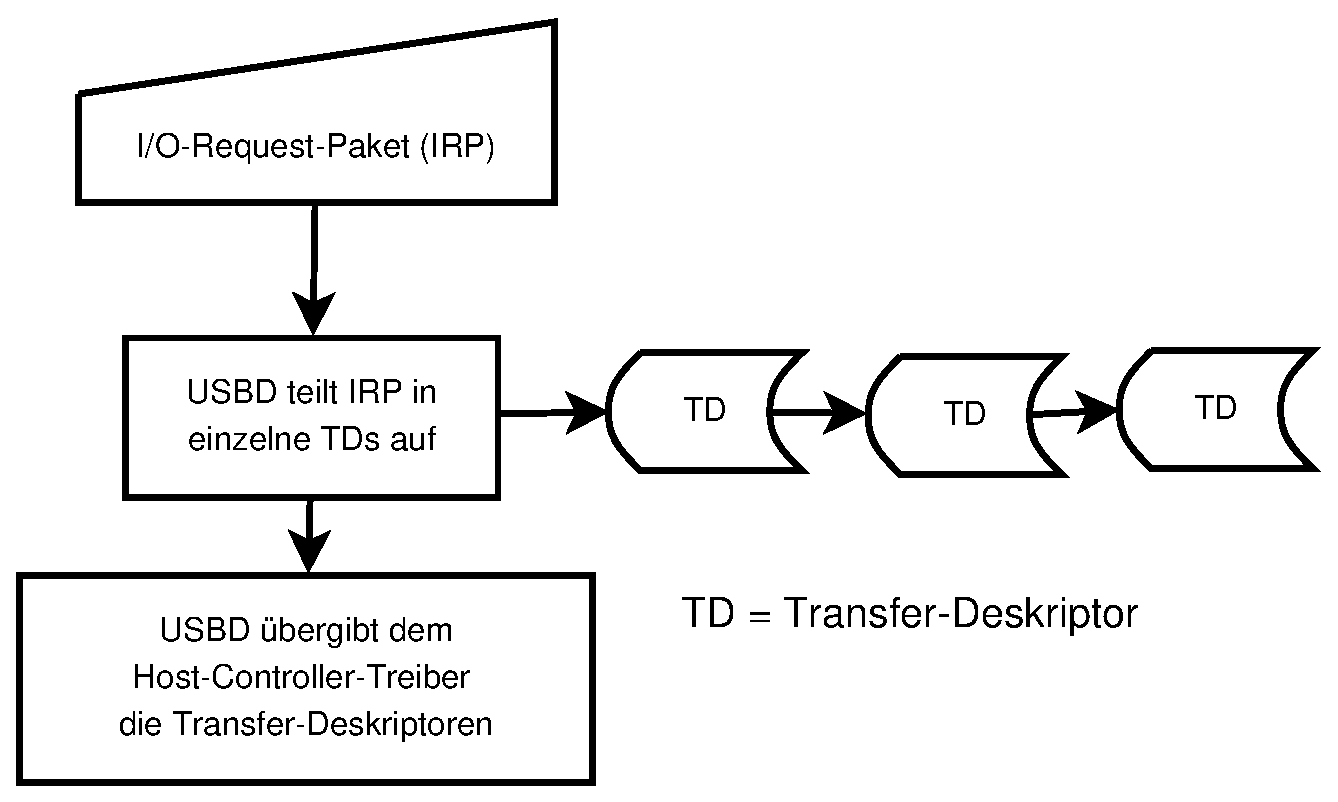
\includegraphics[width=11.5cm]{images/irp}
\caption{Aufteilung der I/O-Request-Pakete in Transfer-Deskriptoren}
\label{irp}
}
\end{figure}
Die Aufteilung ist unter anderem daf�r notwendig, dass die am Bus angeschlossenen
Ger�te mit gleicher Priorit�t behandelt werden k�nnen.
Mehr dazu im n�chsten Absatz \glqq{}Verteilung der Bandbreite\grqq{}.

\subsection{Verteilung der Bandbreite}
\index{Bandbreite}
W�rde ein Treiber zum Beispiel 1 MB Daten an ein Ger�t senden, w�re der
Bus theoretisch bei 12 MBit/s f�r 1,5 s belegt. Betreibt man parallel am Bus
zus�tzlich eine USB-Maus, so k�nnte in dieser Zeit die Maus nicht erreicht und somit
der Mauszeiger nicht aktualisiert werden.
Daher ist es notwendig, dass USB-Nachrichten
durch Segmentierung in einzelne USB-Pakete (\glqq{}Transfer-Deskriptoren\grqq{}) aufgeteilt werden
und einzeln nach und nach abwechselnd mit Paketen von anderen Nachrichten versendet werden. 
Dadurch kann der Host in einer Zeitspanne,
die durch Frames aufgeteilt ist (siehe Kapitel 3.8), mehrere Ger�te ansprechen.
\newline\newline
Mit welcher Strategie die zur Verf�gung stehende Zeit verteilt werden muss, ist in der USB-Spezifikation nicht beschrieben.
Die USB Spezifikation gibt nur an, wieviel Zeit f�r welche Transferart reserviert sein muss (siehe Tabelle \ref{usb_zeiten}).

\begin{table}[h]
\center
\begin{tabular}{|l|l|}
\hline
\rowcolor{Gray}[0.9\tabcolsep]
Transferart & Bandbreite \\ \hline
Control & max. 10\% garantiert \\ \hline
Interrupt und Isochron & max. 90\% garantiert \\ \hline
Bulk & nur bei verf�gbarer Bandbreite \\ \hline
\end{tabular} \caption{Garantierte Bandbreiten der Transferarten} \label{usb_zeiten}
\end{table}

\subsection{Status�berwachung}
\index{Status�berwachung}
Da der USB-Bustreiber alle wichtigen Komponenten verbindet, bietet er sich ideal
f�r die �berwachung des Busses an. Die Auslastung auf dem Bus kann z.B. anhand 
der Anzahl der �bertragenen Pakete ermittelt werden oder auch die korrekte Arbeitsweise der
USB-Ger�te und des Host-Controllers mit speziellen Funktionen der Treiber.
In der USB-Spezifikation ist nicht definiert, welche Informationen �berwacht werden sollen,
es wird nur angeregt, dies an der gerade genannten Stelle im USB-Bustreiber zu integrieren.
\newpage

%Sogenannte USB Debug Monitor, die den Datentransfer f�r eine Analyse
%des Datenstroms aufzeichnen bieten sich ebenfalls an dieser Stelle zu integrieren.

\section{Host-Controller}
\index{Host-Controller}
Der Host-Controller ist verantwortlich f�r die Generierung 
der �bertragungen der einzelnen USB-Pakete, eingepackt in die
Transfer-Deskriptoren.

\subsection{Aufbau und Struktur}

In allen Implementierungen f�hren Host-Controller die gleichen grundlegenden Aufgaben 
hinsichtlich des USB-Busses und seiner verbundenen Ger�te durch. In der USB-Spezifikation
werden die einzelnen Teilkomponenten (Abbildung \ref{host}), die daf�r notwendig
sind, beschrieben.

\begin{figure}[h]
{
\centering
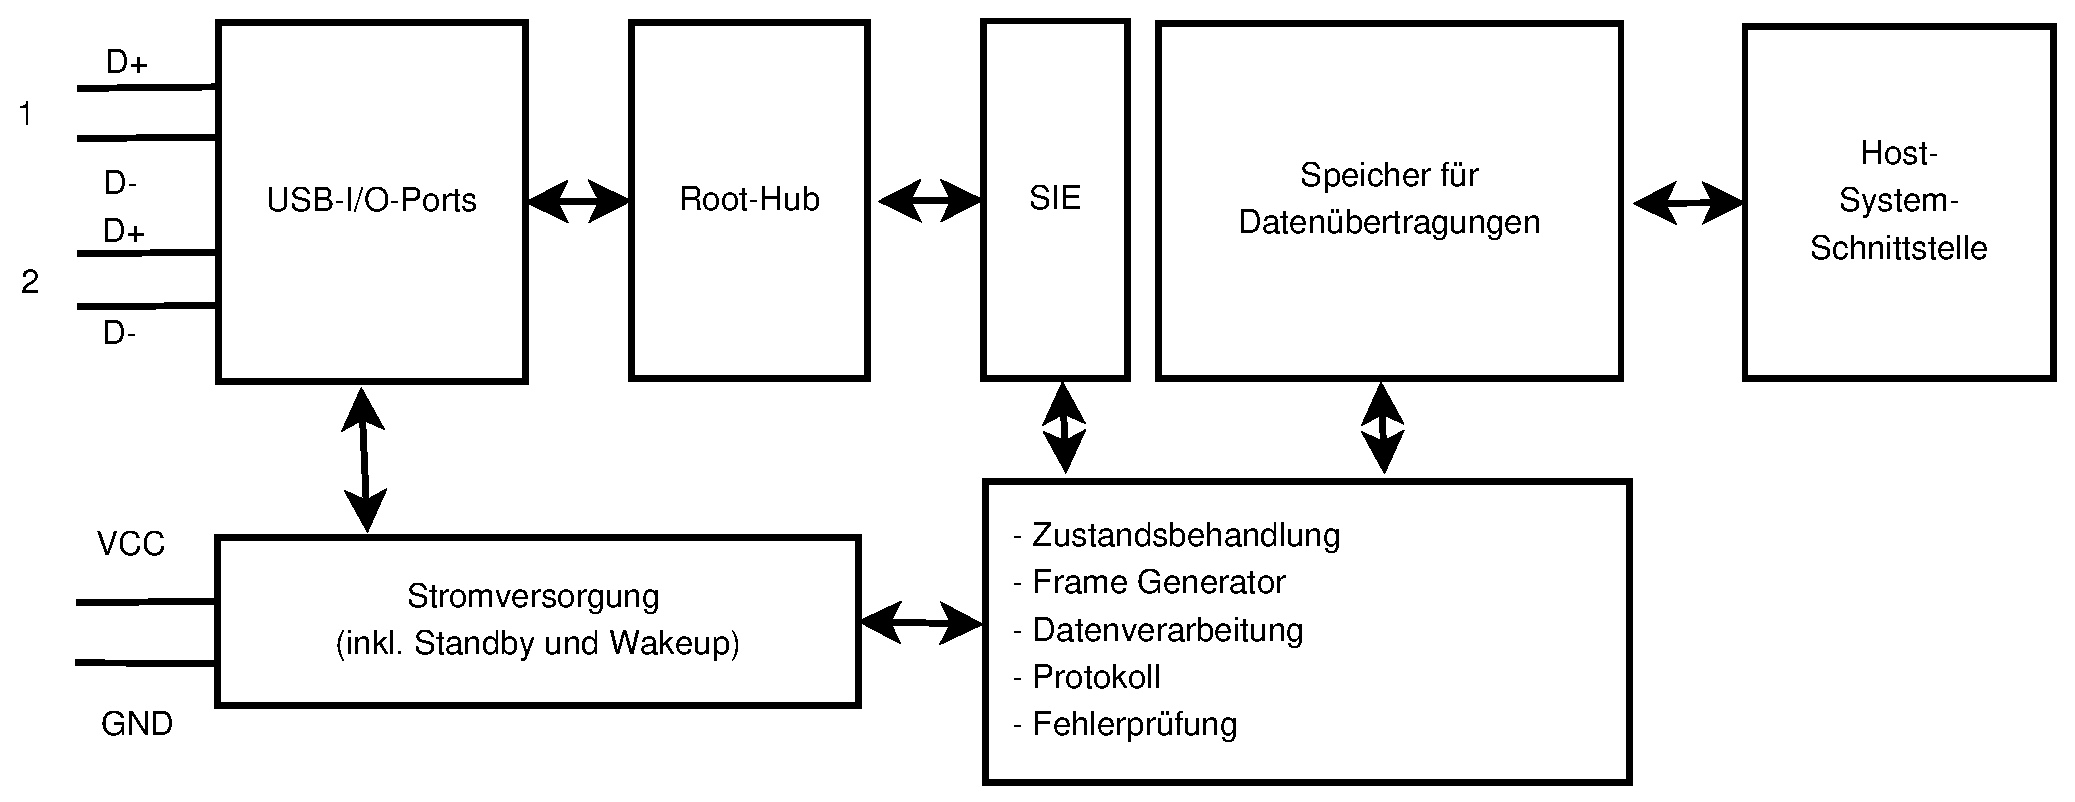
\includegraphics[width=15cm]{images/host}
\caption{Host-Controller Strukturdiagramm}
\label{host}
}
\end{figure}


\index{SIE}
\index{Root-Hub}

\begin{description}
\item[Zustandsbehandlung:] 
Der Host-Controller kann viele Ereignisse und Zust�nde vom USB-Bus
�ber interne Register und Signale anzeigen. Diese Zust�nde
werden vom USB-Stack f�r den Betrieb des USB-Busses ben�tigt.

\item[Serialisierer und Deserialisierer (\glqq{}SIE\grqq{}):] 
Um die Daten �bertragen und empfangen zu k�nnen, muss der Host-Controller,
wie in Kapitel \ref{kap:signal} auf Seite \pageref{kap:signal} beschrieben, die Daten zum Senden serialisieren und codieren
und beim Empfangen wieder decodieren und parallelisieren.


\item[Rahmenerzeugung (\glqq{}Frame Generation\grqq{}):] 
Der Host-Controller ist zust�ndig f�r die Einteilung des Busses in die einzelnen Frames.
Daf�r muss jede Millisekunde ein Start-of-Frame Paket (SOF) mit einer fortlaufenden
Nummer versendet werden.
�ber interne Zeitgeber kann der Host-Controller dies automatisch erledigen.


\item[Datenverarbeitung:] 
Der Host-Controller ist f�r das Empfangen
und das Senden von Daten (USB-Paketen) verantwortlich. 

\item[Protokoll:]
Die passenden Protokollinformationen f�r ausgehende Anfragen m�ssen zusammengesetzt werden und
eingehende Anfragen zerlegt und interpretiert werden.

\item[Fehlerbehandlung bei der �bertragung]
Der Host-Controller muss Datentransportfehler erkennen k�nnen. In
der USB-Spezifikation sind die folgenden Fehlerarten beschrieben:

\begin{itemize}
\item \glqq{}Timeout-Fehler\grqq{} nach Datentransfer. Diese treten auf, wenn die
Endpunktadresse nicht existiert, oder die zu �bertragenden Daten so
fehlerhaft sind, dass diese vom USB-Ger�t nicht interpretiert werden k�nnen.
\item Fehlende oder fehlerhafte Daten:

\begin{itemize}
\item Der Host-Controller sendet oder empf�ngt ein zu kurzes Paket.
\item Ein empfangenes Paket enth�lt eine ung�ltige CRC Pr�fsumme.
\end{itemize}

\item Protokollfehler:
\begin{itemize}
\item Ein ung�ltiges \glqq{}Handshake-Packet\grqq{}.
\item Ein falsches \glqq{}End-of-Packet (EOP)\grqq{}.
\item Ein Bitstuffing-Fehler.
\end{itemize}
\end{itemize}

\item[Entferntes Aufwecken (\glqq{}Wakeup\grqq{}):] 
Das USB-System kann den Bus jederzeit in den Zustand Standby versetzen
und anschlie�end wieder aufwecken.
Daf�r muss der Host-Controller entsprechende Vorrichtungen anbieten.

\item[Root-Hub:] 
Der Root-Hub stellt die Verbindung zwischen dem Host-Controller
und den Anschlussports f�r Ger�te her. Die Arbeitsweise
ist gleich dem Hub (siehe Seite \pageref{kap:hub}). Der einzige Unterschied
besteht in der Anbindung an das System. So ist ein Root-Hub
im Gegensatz zum Hub, der �ber USB angesprochen wird
�ber interne Signale mit dem Host-Controller verbunden.

\item[Host-System-Schnittstelle:] 
Die Schnittstelle f�r den Datenaustausch zwischen dem Host-Controller
und dem Prozessor, auf dem der USB-Stack l�uft.
\end{description}

\subsection{Daten�bertragung mit Host-Controllern} \label{kap:datenuebertragung}
\index{Daten�bertragung}
\index{OHCI}
\index{EHCI}
\index{UHCI}
\index{USB-Nachricht}
\index{Transfer-Deskriptor}
\index{I/O-Request-Paket}
Im vorherigen Abschnitt wurden alle Funktionen,
die ein Host-Controller anbieten muss, kurz beschrieben. F�r die Implementierung
des USB-Stacks in dieser Diplomarbeit soll die Funktionsweise der
Daten�bertragung, speziell f�r Host-Controller in Embedded Systeme, genauer betrachtet werden.
\newline\newline
Wie die �bertragung auf dem Host-Controller genau
funktioniert, ist in dem Hauptdokument der USB-Spezifikation nicht beschrieben.
Dies war die Aufgabe der Host-Controller Hersteller. F�r USB 1.1 wurden
zwei Standards entwickelt, das UHCI (\glqq{}Universal-Host-Controller-Interface\grqq{})  und das
OHCI (\glqq{}Open-Host-Controller-Interface\grqq{}). UHCI kompatible Bausteine
kommen mit weniger Transistoren aus, da dort ein Gro�teil
der Steuerung mit Software erledigt wird. OHCI im Gegenzug verlagert
viele der Verwaltungsaufgaben in die Hardware und bietet daher eine einfachere
Schnittstelle an. UHCI wurde von Intel, und  OHCI
gemeinsam von Compaq, Microsoft und National Semiconductor entwickelt.
F�r USB 2.0 wurde von allen beteiligten Firmen ein gemeinsamer Standard EHCI (Enhanced-Host-Controller-Interface) definiert.
\newline\newline
Obwohl sich alle drei Standards doch sehr unterscheiden, gibt es trotzdem eine gemeinsame Eigenschaft - bedingt dadurch, dass
alle Controller f�r den Einsatz im Computer entwickelt worden sind -
n�mlich die �bergabe der kompletten Transfer-Deskriptoren �ber einen gemeinsamen Arbeitsspeicherbereich
zwischen dem Prozessor und dem Host-Controller. 
\newline\newline
Sendet ein Treiber oder eine Anwendung eine USB-Nachricht ab, so wird direkt ein Speicherbereich
aus dem gemeinsamen Arbeitsspeicher zwischen Prozessor und Host-Controller f�r die Kommunikation genutzt (siehe Abbildung \ref{cpu2host}). Die Software
muss lediglich die Datenstruktur richtig aufbauen, so dass die Hardware die 
einzelnen Transfer-Deskriptoren erreichen kann. Wird der letzte Transfer-Deskriptor
eines I/O-Request-Paketes erfolgreich abgearbeitet, so muss
dies die Hardware nur noch der Software signalisieren, welche dann wiederum dem
Treiber oder der Anwendung meldet, dass die Daten in dem zuvor reservierten
Speicher eingetroffen sind.

\begin{figure}[h]
{
\centering
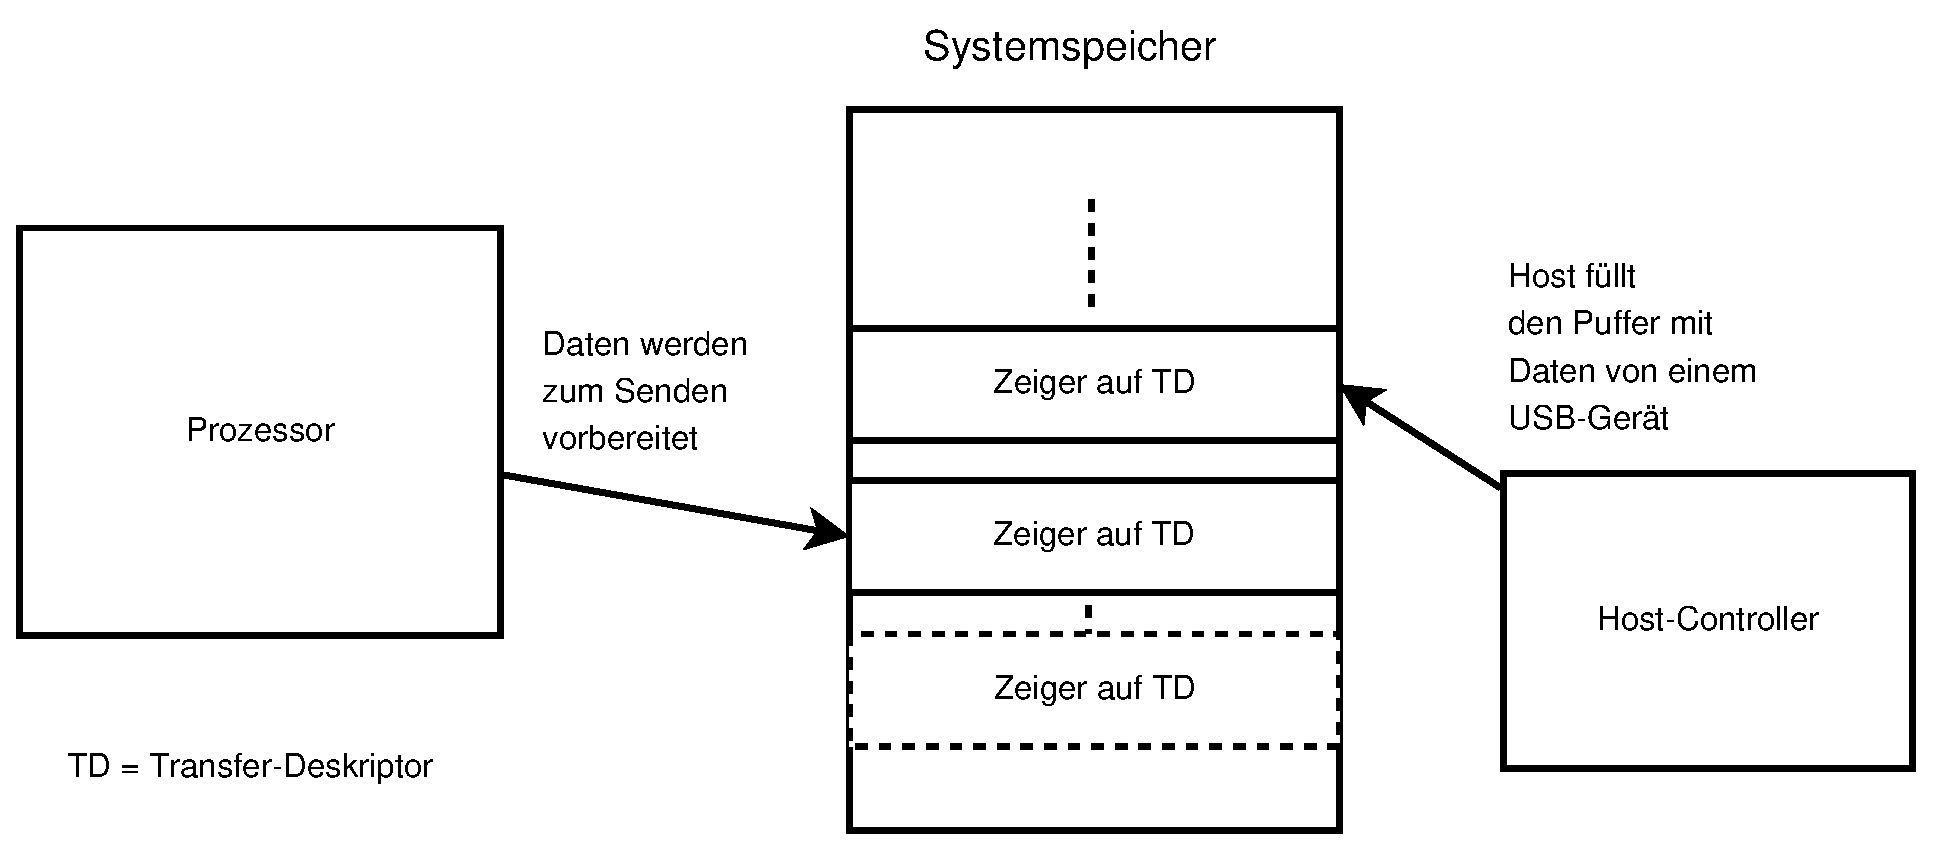
\includegraphics[width=15cm]{images/cpu2host}
\caption{Gemeinsamer Speicher von Prozessor und Host-Controller}
\label{cpu2host}
}
\end{figure}

Bei Mikroprozessoren hingegen muss die �bergabe aber oft �ber I/O-Zugriffe oder spezielle Schnittstellen realisiert
werden, da es dort h�ufig nicht m�glich ist, mit Peripherie Speicherbereiche zu teilen.
Das bedeutet, dass jede �bergebene Transaktion sofort ausgef�hrt werden muss und ein Ergebnis f�r
die weitere Verarbeitung des USB-Pakete-Datenstroms erforderlich ist.
\newline\newline
Damit alle Host-Controller-Typen im USB-Stack genutzt werden k�nnen,
�bergibt der USB-Bustreiber dem Host-Controller-Treiber immer
einzelne Transfer-Deskriptoren. In den Transfer-Deskriptoren
befindet sich aber wiederum ein Zeiger auf das dar�ber liegende
I/O-Request-Paket (siehe Abbildung \ref{td2irp}).
So kann in den Treibern abh�ngig vom Baustein
entschieden werden, wie die Abarbeitung stattfinden soll.

\begin{figure}[h]
{
\centering
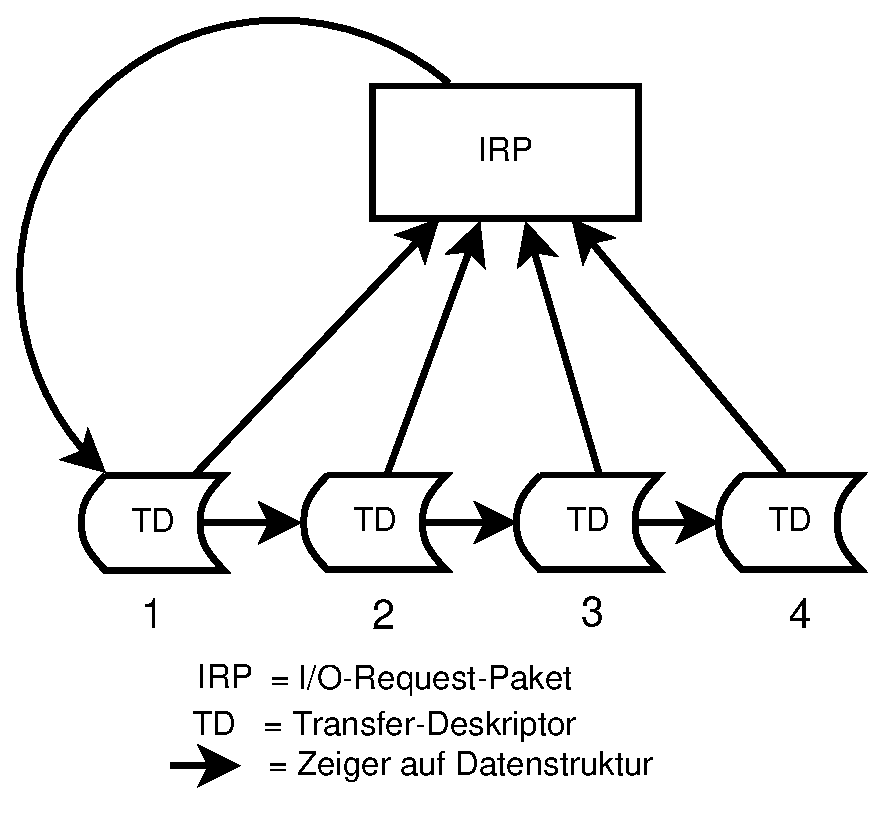
\includegraphics[width=8cm]{images/td2irp}
\caption{Verkettung der Datenstrukturen IRP und TD}
\label{td2irp}
}
\end{figure}

%\subsection{OHCI kompatibler Controller}
%Das OHCI (Open-Host-Controller-Interface) stammt von Compaq, Microsoft
%und National Semiconductor. Implementiert ist OHCI typischerweise in dedizierten Chips�tzen.
%
%\subsubsection{�bertragungsreihenfolge}
%\begin{figure}[h]
%{
%\centering
%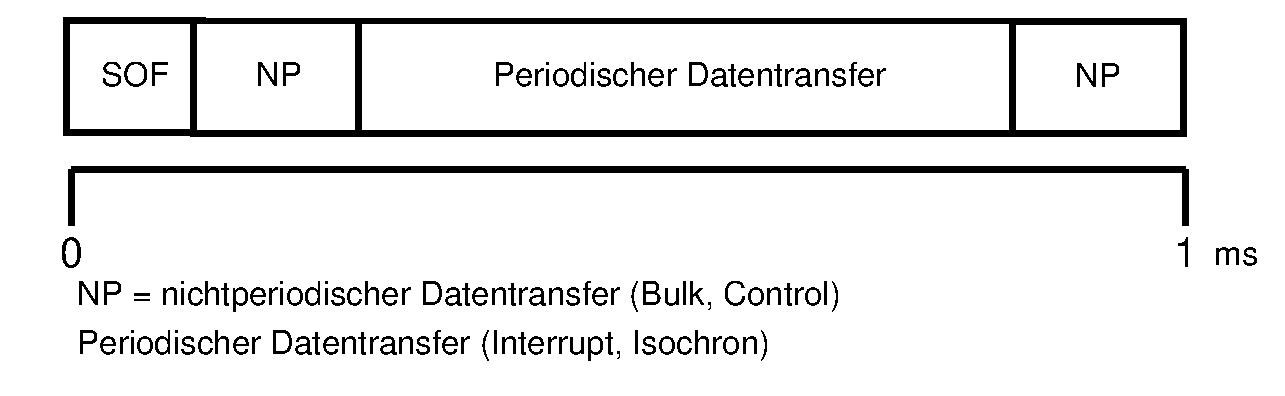
\includegraphics[width=14cm]{images/ohci_zeit}
%\caption{�bertragungsreihenfolge OHCI}
%\label{ohci_zeit}
%}
%\end{figure}
%\subsubsection{Transfermechanismus}
%\begin{figure}[h]
%{
%\centering
%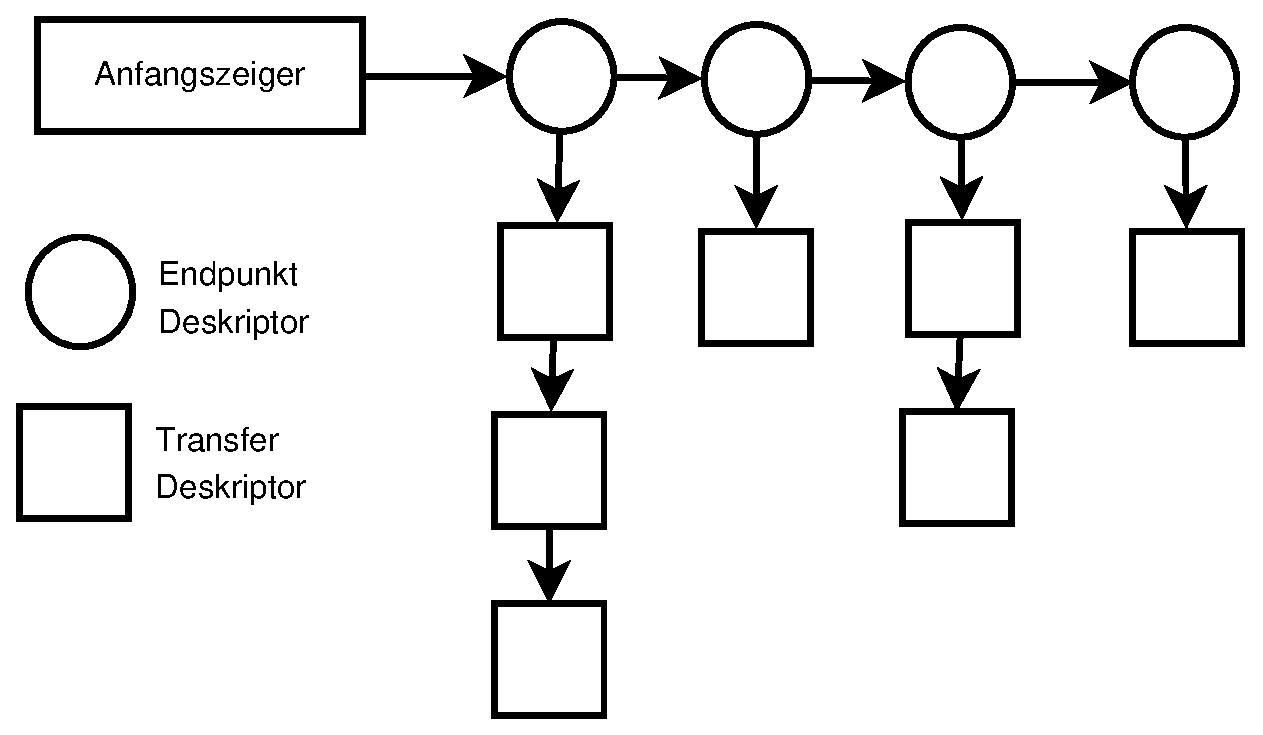
\includegraphics[width=11cm]{images/ohci}
%\caption{Transfermechanismus OHCI}
%\label{ohci}
%}
%\end{figure}
%\subsubsection{Enpunkt-Deskriptoren}
%\subsubsection{Transfer-Deskriptoren}
%\subsubsection{OHCI Register}
%\subsection{UHCI kompatibler Controller}
%Die UHCI (Universal-Host-Controler-Interface) Spezifikation wurde von Intel erstellt.
%Das Interface ist ebenfalls wie das OHCI meist in Chips�tzen integriert. Die Komplexit�t
%des UHCI wird von Intel mit etwa 10K Gates angegeben.
%\subsubsection{�bertragungsreihenfolge}
%\subsubsection{Frame-Listen}
%\subsubsection{Transfer-Mechanismus}
%\subsubsection{Transfer-Deskriptoren}
%\subsubsection{Queue-Heads}
%\subsubsection{UHCI Register}
%
%\subsection{EHCI kompatibler Controller}
%
%Mit der Spezifikation USB 2.0 wurde gleich ein Standard Host-Controller ver�ffentlicht,
%welcher die Erweiterungen zum High-Speed Modus beinhaltet und gleichzeitig Abw�rtskompabilit�t gew�hrleisten
%soll.
%
%
%\subsubsection{Architektur}
%\subsubsection{Host-Controller-Routing-Strategie}
%\subsubsection{Datenstrukturen}
%
%\subsection{Phillips kompatible Controller}
%
%Es gibt auch Controller die diesem Standard nicht entprechen. Vorallem im Embedded Bereich,
%denn hier hat man selten einen gemeinsamen speicherbereich. Meistens eine
%Port oder eine andere schnittstelle
%
%beispiel phillips mach beides mit den PTD

%\section{Integrierter Root-Hub-Controller}

%Die Aufgabe eines USB Hubs ist das Anzeigen des aktuellen Status der Ports
%und �nderungen an ihnen. Aufgrund dieser Informationen kann der Hub Treiber
%den Host �ber �nderungen informieren, und der Host kann entsprechend
%eine Enumeration oder mit dem Entfernen von Datenstrukturen f�r ein
%entferntes Ger�t beginnen. 
%\newline\newline
%Da ein Host-Controller f�r die Signalisierung von �nderungen an dem
%abgehenden USB-Ports meistens Interrupt Signale und interne Status Register hat,
%welche f�r die Aufgaben des Root-Hubs notwendig sind,
%simuliert man dort einen echten USB-Hub, so dass man die Host-Ports �ber
%den gleichen Hubtreiber wie die f�r ein USB-Hub ansteuern kann und sich doppelte Arbeit spart.

\newpage
\section{Bandbreitenabsch�tzung}
\index{Daten�bertragungsrate}
\index{Bulk-Transfer}
Bei der Konzeption von USB-Ger�ten ist die Frage der maximalen
Daten�bertragungsrate oft von Interesse. Daher wird in diesem Abschnitt
eine Beispielrechnung vorgef�hrt, um zu zeigen, auf welche
Faktoren und Parameter geachtet werden muss, um die Kapazit�ten
des USB-Busses vollst�ndig auszunutzen.
\newline\newline
In der USB-Spezifikation sind die drei Ger�teklassen
Low-Speed-Ger�te (bis 1,5 MBit/s), Full-Speed-Ger�te (bis 12 MBit/s)
und High-Speed-Ger�te (bis 480 MBits/s ab USB Version 2.0) definiert.
Diese Angabe bezieht sich aber auf die physikalische maximale �bertragungsrate.
Soll die tats�chliche Datenrate ermittelt werden, m�ssen einige Parameter beachtet werden.
Im folgenden Beispiel wird eine Rechnung f�r einen Bulk-Transfer mit einem Full-Speed-Ger�t (12 MBit/s)
durchgef�hrt.
\newline\newline
In Kapitel \ref{pakzei} (Seite \pageref{pakzei}) wurde bereits beschrieben, dass Daten nach dem Start-of-Frame-Paket (SOF) versendet werden. 
Da das SOF-Paket jede Millisekunde vom Host generiert wird, bedeutet dies bei Full-Speed-Ger�ten (12 MBit/s),
dass maximal 12000 Bit (je Bit 83,33 ns) pro Millisekunde �bertragen werden k�nnen.
Die Gr��e der Daten-Pakete ist wiederum abh�ngig von der maximalen Endpunkt-Tiefe (siehe Taballe \ref{usb_bandbreite_full} und \ref{usb_bandbreite_high}), welche 
durch die Transferart bestimmt wird. Bei dem gew�hlten Bulk-Transfer mit Full-Speed-Ger�ten
kann ein Endpunkt-FIFO maximal 64 Byte (= 512 Bit) gro� sein. 
Ein weiterer Faktor f�r die Ermittlung der maximalen Daten�bertragungsrate ist der Overhead (Protokoll-Overhead und Bit-Stuffing),
der f�r ein Daten-Paket ben�tigt wird. F�r einen Bulk-Endpunkt ist dieser 13 Byte (= 104 Bit) gro�.
\newline\newline
Der entscheidendste Faktor ist aber der, wie oft ein Daten-Paket w�hrend einer Millisekunde an einen Endpunkt
gesendet werden kann.
Aus den Tabellen \ref{usb_bandbreite_full} und \ref{usb_bandbreite_high} kann entnommen werden, dass ein Bulk-Endpunkt bis zu 19 mal pro Frame angesprochen werden kann.
Wie dieser Wert zustande kommt, wird mit der nachstehenden Rechnung gezeigt:

\begin{eqnarray}
\text{max. �bertragungen} & = & \frac{\text{max. Anzahl Bits pro ms}}{\text{Overhead + max. FIFO-Tiefe}} \\[5mm]
\text{max. �bertragungen} & = & \frac{12000\text{ Bit}}{104\text{ Bit} + 512\text{ Bit}} \\[5mm]
& = & 19,48 \text{ �bertragungen pro Millisekunde}
\label{max_datenrate}
\end{eqnarray}

Mit der maximalen Anzahl an �bertragungen pro Frame kann im n�chsten Schritt die Berechnung der maximalen �bertragungsrate
durchgef�hrt werden.

\begin{eqnarray}
\text{max. �bertragungsrate} & = & \text{max. �bertragungen} * \text{max. FIFO-Tiefe}\\[5mm]
\text{max. �bertragungsrate} & = & 19 \text{ pro ms} * 512\text{ Bit} \\[5mm]
& = & 9,728\text{ MBit/s}
\end{eqnarray}

Mit 19 Paketen kann man also eine �bertragungsrate von ca. 9,7 MBit/s erreichen.
Die angenommenen 19 Pakete sind die theoretisch maximal M�glichen.
Ob alle Pakete innerhalb eines Frames auch versendet werden k�nnen,
h�ngt von dem eingesetzten Host-Controller ab. Wie bereits erw�hnt,
werden die Daten immer nach den SOF-Paketen, welche meist von den Host-Controllern
automatisch generiert werden, versendet.
Oft kann man sich das Absenden durch einen Interrupt signalisieren lassen.
Liegen  die Daten zu dem Zeitpunkt des Signalisierens bereits im Speicher, den der Host zum Versenden benutzt,
werden die ersten 64 Byte Daten plus Overhead f�r das erste Paket sofort versendet.
\newline\newline
Der weitere Verlauf ist abh�ngig von der Art des Host-Controllers.
Wie in Kapitel \ref{kap:datenuebertragung} auf Seite \pageref{kap:datenuebertragung} beschrieben, gibt es prinzipiell zwei Arten.
Die einen, bei den Pakete direkt aus einem gemeinsamen Speicher mit dem Prozessor �bertragen werden k�nnen,
und die anderen, bei denen jedes Paket �ber eine I/O-Schnittstelle �bergeben werden muss. 
F�r die Ermittlung der Datenrate werden beide F�lle f�r den weiteren Verlauf beschrieben.
\newline\newline
\textbf{1. Fall: Host nutzt gemeinsamen Speicher mit dem Prozessor: }
Wenn alle Pakete im Speicher bereit liegen, kann der Host-Controller nacheinander alle
Daten versenden.
\newline\newline
\textbf{2. Fall: Dem Host werden die Pakete �ber eine I/O-Schnittstelle �bergeben: }
Viele Host-Controller dieser Art bieten zwei Speicherbereiche f�r die Daten�bertragung an.
Dadurch kann, w�hrend der Inhalt des einen Speichers �bertragen wird, der zweite mit Daten gef�llt werden.
Dies wechselt sich immer ab, bis der Transfer beendet ist. F�r die I/O-Schnittstelle bedeutet dies aber, dass innerhalb
von min. 43 $\mu$s (512*83,33 ns) 64 Byte �bertragen werden m�ssen, damit die Daten rechtzeitig
in dem zweiten Speicher bereitstehen. Bei einem 8-Bit breiten I/O-Bus ben�tigt man
so, wenn man f�r den Verwaltungs-Overhead den Faktor 3 annimmt (Lese-, Schreib- und Adresssignale setzen), 
eine I/O-Geschwindigkeit von mindestens 5 MHz. 
\newline\newline
Angenommen, der Host-Controller hat nur einen Speicherbereich zum �bertragen der Daten,
so entsteht immer eine kleine Pause zwischen zwei Paketen, das ist wiederum die Zeit, die f�r das Auff�llen des Speichers notwendig 
ist.
%\newline\newline
%Die komplett verf�gbare Bandbreite kann nur genutzt werden wenn alle diese Parameter
%bedacht werden. 
\index{�bertragungsrate}

\begin{table}[h]
\center
\begin{tabular}{|l|L{2cm}|L{3cm}|L{3cm}|l|}
\hline
\rowcolor{Gray}[0.9\tabcolsep]
Transferart & Overhead\newline(Byte) & max. FIFO-Tiefe (Byte) & Transfers pro Frame (Byte) & Bandbreite \\ \hline
Control (OHCI) & 45 & 64& max. 13 & 6,6 MBit/s\\ \hline
Control (UHCI) & 45 & 64& 1 & 512 KBit/s\\ \hline
Interrupt & 13 & 64& 1 & 512 KBit/s \\ \hline
Bulk & 13 & 64 & max. 19 & 9,7 MBit/s \\ \hline
Isochron & 9 & 1023 & 1 & 8,2 MBit/s \\ \hline
\end{tabular} \caption{Maximale Datenrate f�r Full-Speed-Ger�te} \label{usb_bandbreite_full}
\end{table}



\begin{table}[h]
\center
\begin{tabular}{|l|L{2cm}|L{3cm}|L{3cm}|l|}
\hline
\rowcolor{Gray}[0.9\tabcolsep]
Transferart & Overhead\newline(Byte) & max. FIFO-Tiefe (Byte) & Transfers pro Frame (Byte) & Bandbreite \\ \hline
Control (EHCI) & 45 & 64& 1 & 4,0 MBit/s\\ \hline
Interrupt & 13 & 3x1024 & 1 & 192 MBit/s \\ \hline
Bulk & 13 & 512 & max. 12 & 384 MBit/s \\ \hline
Isochron & 9 & 3x1024 & 1 & 192 MBit/s \\ \hline
\end{tabular} \caption{Maximale Datenrate f�r High-Speed-Ger�te} \label{usb_bandbreite_high}
\end{table}


	
\chapter{Implementierung des USB-Host-Stack}

Nach den im vorherigen Kapitel beschriebenen Komponenten
und deren Aufgaben im USB-Host-Stack soll auf 
die Implementierung des gesamten USB-Systems eingegangen werden.
Erkl�rt wird unter anderem die Verzeichnisstruktur, die API f�r die Anwendungen, die Treiber und 
die Host-Controller und die Struktur des Algorithmus
zur Aufteilung von I/O-Requests in Transfer-Deskriptoren.
Im Unterkapitel \glqq{}Integration in ein eigenes Projekt\grqq{}(Seite \pageref{integration}) wird gezeigt,
was bei der Integration des USB-Stacks in eine eigene Anwendung wichtig ist.

\section{Eigenschaften}
\index{USB-Stack}
Der USB-Stack soll flexibel auf den verschiedensten Prozessorarchitekturen
einsetzbar sein. Da der gesamte Quelltext mit allen Treibern, Modulen und Bibliotheken
f�r ein Embedded System zu gro� w�re und das meiste f�r ein Projekt auch �berfl�ssig 
ist, wurde der Stack so aufgebaut, dass nur die absolut notwendigen Teile
herausgenommen und miteinander verkn�pft werden k�nnen. 
\newline\newline
Es wurde immer versucht, einen Kompromiss zwischen Einfachheit und Umfang des Codes
zu schaffen. Beispielsweise sind die USB-Ger�te-Treiber dynamisch in
den Stack eingebunden, da hier mehrere Treiber gleichzeitig existieren k�nnen. Die
Host-Controller-Treiber wiederum werden statisch bei der Compilierung fest
in das Programm integriert, da ein Embedded System mit einem einzigen Host-Controller
auskommt und dadurch wieder weniger Arbeitsspeicher und Programmcode f�r die Verwaltung
der Host-Controller-Treiberstrukturen ben�tigt wird.
\newline\newline
Die wichtigsten Eigenschaften des USB-Stacks sind:
\begin{enumerate}
\item Niedriger RAM Verbrauch (ca. 200 Byte)
\item Kleine Codegr��e (ab 4 KB)
\item Die Module und Treiber sind flexibel kombinierbar
\item Fertige Klassen-, Ger�tetreiber und Bibliotheken f�r USB-Ger�te
\item Hub-, Massenspeicher-, HID-Treiber
\item uclibusb f�r USB-Ger�te-Bibliotheken (Beispiel f�r FT232)
\item Einfache Host-Controller-Schnittstelle 
\item Bereits auf kleinen 8 Bit-Prozessoren einsetzbar
\item Alle Quelltexte sind in C geschrieben
\end{enumerate}
Im n�chsten Abschnitt wird auf die Unterteilung der einzelnen Module eingegangen.

\section{Modul�bersicht} \label{kap:moduluebersicht}
\index{Module}
Durch eine geschickte Trennung der Quelltexteinheiten ist es m�glich,
einen Stack mit den nur absolut notwendigen Teilen zusammenzustellen.
In Abbildung \ref{module_c} wird gezeigt, wie die einzelnen Module 
aufeinander aufbauen und voneinander abh�ngig sind.

\begin{figure}[h]
{
\centering
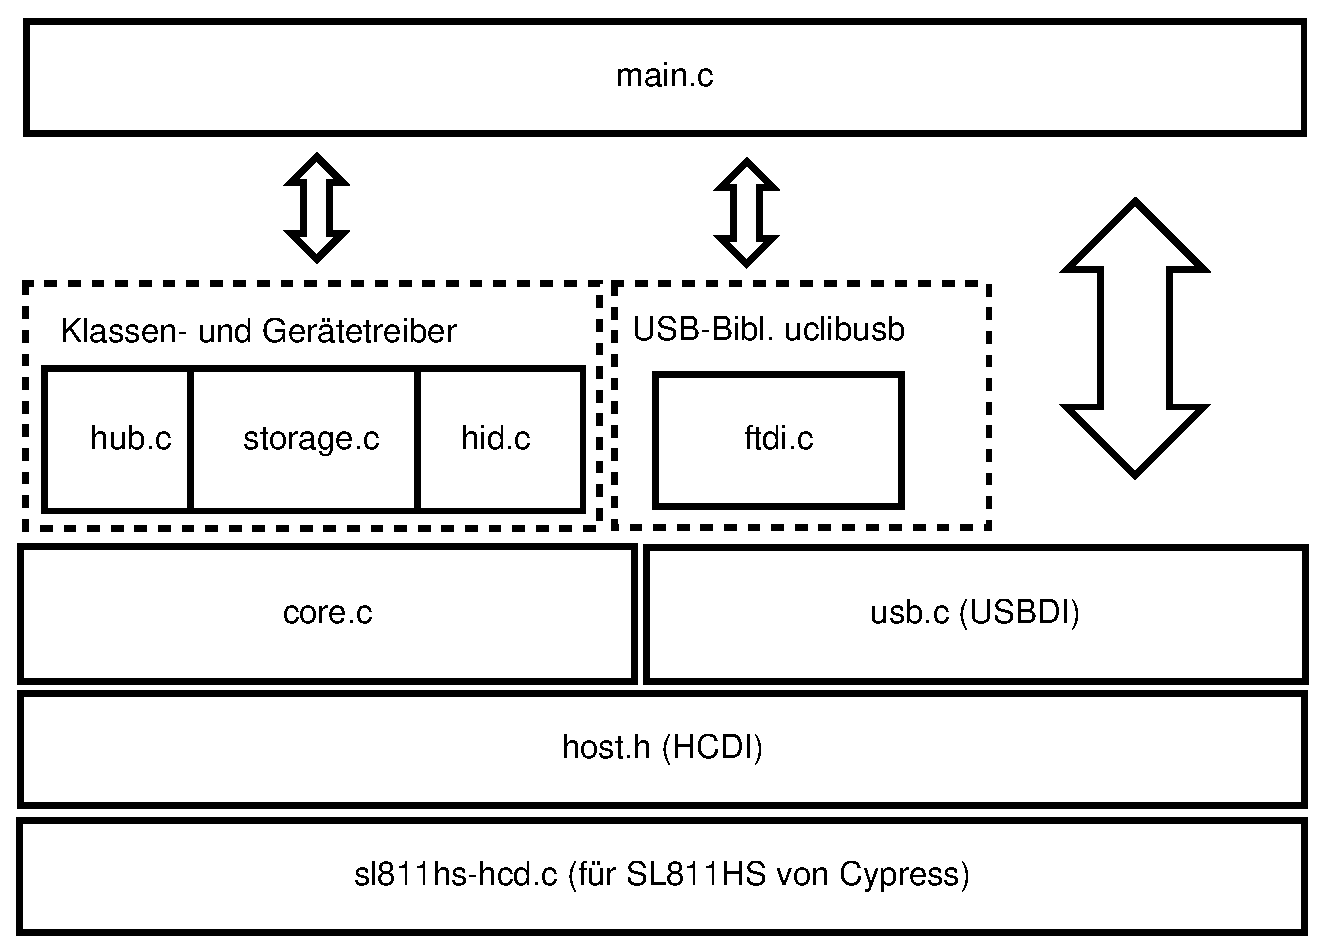
\includegraphics[width=11cm]{images/module_c}
\caption{C-Module des USB-Stacks}
\label{module_c}
}
\end{figure}
\index{Host-Controller-Treiber}
\index{Klassentreiber}
\index{Ger�tetreiber}
Auf der untersten Ebene des USB-Stacks befindet sich der Host-Controller-Treiber (z.B. \textbf{sl811hs-hcd.c} f�r den
Host-Controller SL811HS von Cypress,
der im Rahmen dieser Diplomarbeit entwickelt worden ist.),
welcher die Funktionen aus der Header-Datei \textbf{host.h} anbieten muss.
�ber diese Funktionen kann der USB-Stack Anfragen absenden und empfangen.
Im Host-Controller-Treiber (HCD) m�ssen zudem die Funktionen f�r
den Root-Hub integriert sein.
In der Datei \textbf{core.c} befinden sich alle Funktionen f�r die Verwaltung
und Steuerung des Busses (Treiber bzw. Ger�te an- und abmelden, etc.).
Die Kommunikationsfunktionen f�r USB-Ger�te bietet der USB-Stack in der Datei \textbf{usb.c} an.
\newline\newline
Neben den Funktionen f�r die direkte Kommunikation existieren
noch Treiber. Die Treiber k�nnen in zwei Gruppen
aufgeteilt werden, die Klassen- und Ger�tetreiber. F�r Ger�te,
bei denen
kein eigener Treiber ben�tigt wird, gibt es die M�glichkeit,
eine Bibliothek anzubieten, welche im Ordner \textbf{uclibusb} - angelehnt
an das Konzept des bekannten Projektes libusb \cite{libusb} - gesammelt werden.

\section{Verzeichnisstruktur}
\index{Verzeichnisse}
F�r den USB Stack wurde folgende Verzeichnisstruktur angelegt:

\begin{itemize} 
\item \textbf{arch} Beispielimplementierungen f�r verschiedene Mikrocontroller
\item \textbf{boards} Schaltplan, Platinenlayout, etc. f�r die Evaluationsschaltung
\item \textbf{core} USB-Kern-Funktionen
\item \textbf{drivers} USB-Treiber (Ger�te und Klassen)
\item \textbf{host} Host-Controller-Treiber 
%\item \textbf{hwmon} Hardware Monitor f�r USB Host Controller 
\item \textbf{lib} Zusatzfunktionen, Typendefinitionen, etc.
\item \textbf{uclibusb} USB-Bibliotheken f�r USB-Ger�te
\item \textbf{usbspec} Datentypen und -formate der USB-Spezifikation
\item \textbf{doc} Doxygen Dokumentation und die Diplomarbeit als Beschreibung
\end{itemize}


\section{�berblick der Schnittstellen}
\index{API}
Die Softwareschnittstellen des USB-Stacks sind
in drei Gruppen aufgeteilt (Abbildung \ref{api}). 
In der untersten Gruppe, sind die Funktionen definiert, die ein Host-Controller-Treiber
zur Verf�gung stellen muss. Die Zweite dr�ber liegende Gruppe bildet das USB-Bustreiber-Interface (USBDI), welches
Funktionen f�r die Kommunikation der Ger�te- und
Treiberverwaltung anbietet. In der obersten Gruppe ist schlie�lich
die Schnittstelle eines USB-Ger�te- bzw. USB-Klassen-Treibers beschrieben.

\begin{figure}[h]
{
\centering
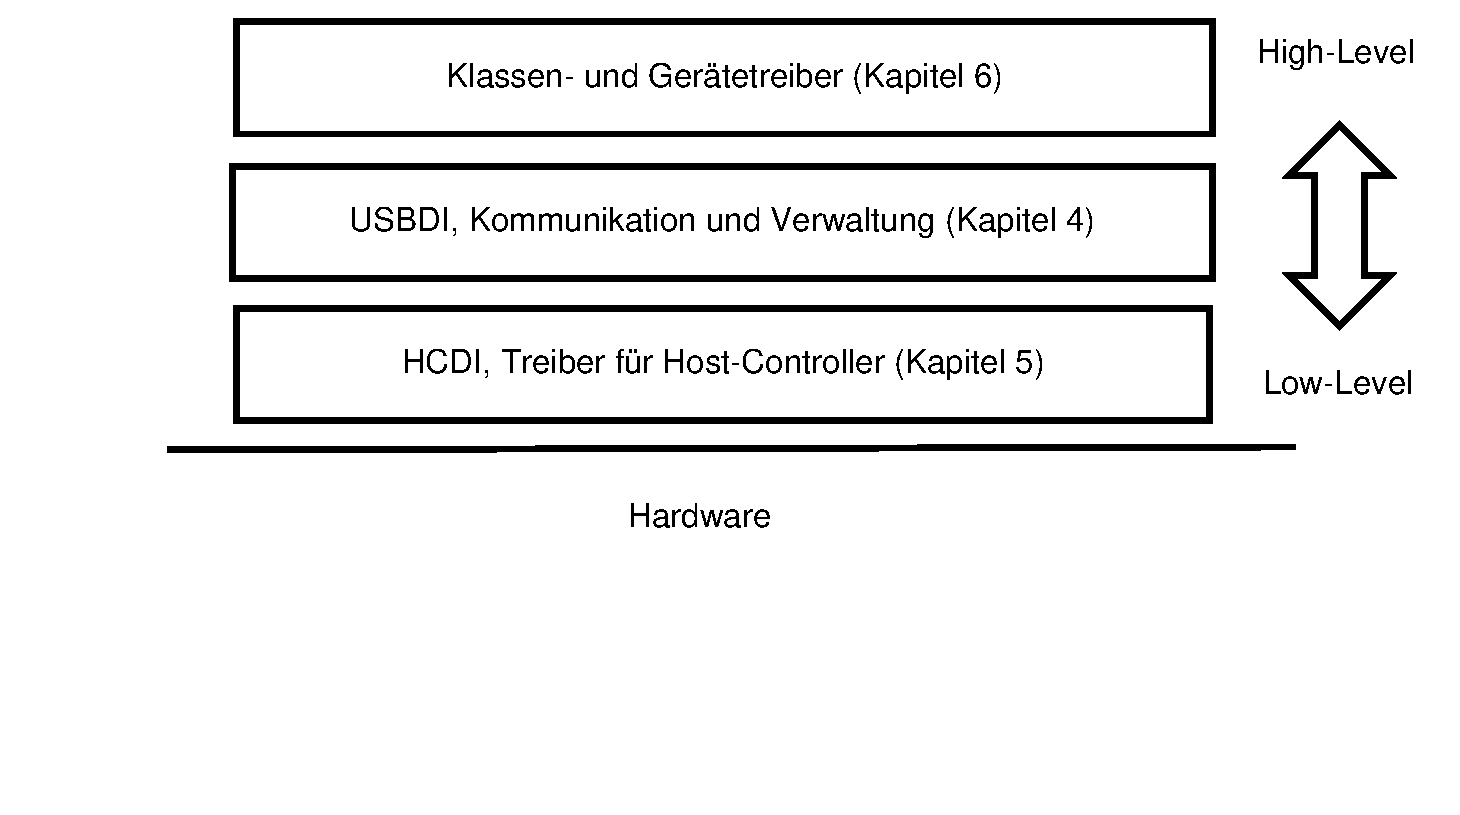
\includegraphics[width=15cm]{images/api}
\caption{USB-Stack-Schnittstellen}
\label{api}
}
\end{figure}
\subsection{HCDI (Host-Controller-Treiber-Schnittstelle)}
\index{Host-Controller-Treiber}
%Im Gegensatz zu einem USB-Ger�te-Treiber gibt es keine Datenstruktur f�r
%einen Host-Treiber, die dem USB-Stack �bergeben werden muss.
Wie in der Modul�bersicht (Abschnitt \ref{kap:moduluebersicht}) bereits erw�hnt,
ist ein einziger Host-Controller f�r die Anbindung mehrerer USB-Ger�te ausreichend.
Deswegen wird der Treiber statisch mit in das Programm gelinkt. Damit
der USB-Stack auf den Host-Controller �ber den Treiber zugreifen kann,
m�ssen die folgenden zwei Funktionen exakt so angeboten werden.

\begin{table}[h]
\center
\begin{tabular}{|l|l|}
\hline
\rowcolor{Gray}[0.9\tabcolsep]
Funktion & Aufgabe\\ \hline
void hcdi\_init() & Host-Controller initieren\\ \hline
u8 hcdi\_enqueue(usb\_transfer\_descriptor *td) & Transfer-Deskriptor �bertragen \\ \hline
%u8 hcdi\_dequeue(usb\_transfer\_descriptor *td) & �bertragung abbrechen \\ \hline
\end{tabular}
\caption{HCDI - Host-Controller-Treiber-Interface [host.h]}
\label{usb_device_add}
\end{table}
\index{host.h}
Die Initialisierungsfunktion wird vom Kern direkt nach dem Starten aufgerufen.
In ihr k�nnen Host-Controller spezifische Register entsprechend
beschrieben werden, so dass sich der Baustein ebenfalls
in einem initialisierten Zustand befindet
und mit der Arbeit beginnen kann. Hier fallen meistens Arbeiten
wie Interruptmasken setzen, Reset-Prozesse ausl�sen, etc. an.
F�r die Daten�bertragung wie in Kapitel \ref{kap:datenuebertragung} auf Seite \pageref{kap:datenuebertragung} beschrieben
muss die Funktion \textit{hcdi\_enqueue} implementiert werden.
Als Parameter erh�lt sie Zeiger auf Transfer-Deskriptoren. F�r die Erkennung von neuen Ger�ten ist der entsprechende
Root-Hub-Treiber zust�ndig. Mehr dazu in Kapitel \ref{{kap:roothub}} auf Seite \pageref{kap:roothub}.


\subsection{USBDI (USB-Bustreiber-Schnittstelle)}
\label{kap:usbdi}
\index{USB-Ger�te-Treiber}
\index{USBDI}
\index{USB-Bustreiber-Schnittstelle}
Die Struktur der USBDI-API ist �hnlich der des GNU/Linux Kernels \cite{kernel}
und der Bibliothek libusb \cite{libusb}. F�r den Entwickler hat 
das zum Einen den Vorteil, dass er sich, wenn er sich mit einer der beiden Schnittstellen bereits
auskennt, leichter in den USB-Stack einarbeiten kann. Zum Anderen
k�nnen Bibliotheken auf einem PC entwickelt werden und anschlie�end
mit kleinen Anpassungen in den USB-Stack integriert werden.
\newline\newline
\textbf{Kommunikation mit Ger�ten}
\newline\newline
Bevor auf ein USB-Ger�t zugegriffen werden kann, wird
ein Zeiger vom Typ \textit{usb\_device} (siehe Listing \ref{lst:usb_dev_struct}) auf das Ger�t ben�tigt.
\lstset{language=C}
\begin{lstlisting}[caption={USB-Ger�te-Datenstruktur, core.h},label={lst:usb_dev_struct},
captionpos=b,
basicstyle=\ttfamily\fontsize{10}{12}\selectfont,
commentstyle=\fontsize{10}{12}\selectfont]
typedef struct usb_device_t usb_device;
struct usb_device_t {
  /* Ger�teinfos */
  u8  address;	     
  u8  fullspeed;
  /* USB Ger�te Desriptor */
  u8  bMaxPacketSize0;
  u8  bDeviceClass;
  u8  bDeviceSubClass;
  u8  bDeviceProtocoll;
  u32 idVendor;
  u32 idProduct;
  u32 bcdDevice;
  u8  bNumConfigurations;
  /* Ende USB Ger�te Desriptor */

  /* Endpunkte */
  u8 epSize[16];
  u8 epTogl[16];

  /* Zeiger auf n�chstes Ger�t im Stack */
  usb_device *next;
};
\end{lstlisting}

Dieser Zeiger ist kein explizites \glqq{}Handle\grqq{} auf das Ger�t,
sondern ein direkter Verweis auf die Ger�tedatenstruktur.
Mit Hilfe der Funktionen \textit{usb\_open()} und \textit{usb\_open\_class()} (siehe Tabelle \ref{usb_device_add_open})
kann solch ein Zeiger ermittelt werden.
Kann das Ger�t nicht gefunden werden oder ist es bereits von einem anderen Treiber bzw. Prozess
reserviert, so erh�lt man eine \textit{NULL} 
als R�ckgabewert. 
Weiterhin besteht noch die M�glichkeit, in den internen Ger�telisten des USB-Kerns
selbst nach dem Ger�t zu suchen. Mehr dazu in Kapitel 6.
\newline\newline
Wurde das gew�nschte Ger�t gefunden, k�nnen mit den Funktionen aus der Tabelle \ref{usb_uebertragung}
Daten versendet und empfangen werden. 
Wird die Verbindung zu einem Ger�t nicht mehr ben�tigt, reicht ein Aufruf der Funktion \textit{usb\_close},
um das Ger�t wieder f�r andere Anwendungen oder Treiber freizugeben.

\begin{table}[h]
\center
\begin{tabular}{|l|l|}
\hline
\rowcolor{Gray}[0.9\tabcolsep]
Funktion & Aufgabe\\ \hline
usb\_open(u32 vendor\_id, u32 product\_id) & Ger�t mit Hersteller- und Produkt-ID finden\\ \hline
usb\_open\_class(u8 class) & Ger�t mit Klassencode finden\\ \hline
usb\_close(usb\_device *dev)  & Verbindung mit einem Ger�t beenden\\ \hline
\end{tabular}
\caption{USBDI - Verbindung zum Ger�t aufbauen [usb.h]}
\label{usb_device_add_open}
\end{table}

\begin{table}[h]
\center
\begin{tabular}{|l|}
\hline
\rowcolor{Gray}[0.9\tabcolsep]
Funktion \\ \hline
usb\_control\_msg(usb\_device *dev, char *buf, u8 size, u8 timeout) \\ \hline
usb\_control\_msg(usb\_device *dev, char *buf, u8 size, u8 timeout) \\ \hline
usb\_bulk\_write(usb\_device *dev, u8 ep, char *buf, u8 size, u8 timeout) \\ \hline
usb\_int\_read(usb\_device *dev, u8 ep, char *buf, u8 size, u8 timeout) \\ \hline
usb\_int\_write(usb\_device *dev, u8 ep, char *buf, u8 size, u8 timeout)  \\ \hline
usb\_isochron\_read(usb\_device *dev, u8 ep, char *buf, u8 size, u8 timeout)  \\ \hline
usb\_isochron\_write(usb\_device *dev, u8 ep, char *buf, u8 size, u8 timeout) \\ \hline
\end{tabular}
\caption{USBDI - Kommunikation mit Ger�t [usb.h]}
\label{usb_uebertragung}
\end{table}
\index{usb.h}
Daten k�nnen mit den Funktionen aus der Tabelle \ref{usb_uebertragung} �bertragen werden.
Was die Parameter der Funktionen bedeuten, wird wie folgt beschrieben:

\begin{itemize}
\item \textbf{usb\_device *dev} Zeiger auf das Ger�t
\item \textbf{u8 ep} Endpunkt f�r die Kommunikation
\item \textbf{char *buf} Speicher f�r zu sendende oder zu empfangende Daten
\item \textbf{u8 size} Anzahl der zu sendenden oder zu empfangenden Daten (in Byte)
\item \textbf{u8 timeout} Abbruchszeit bei fehlerhafter �bertragung (in Millisekunden)
\end{itemize}

Beim Control-Transfer muss im Gegensatz zu den anderen Transferarten keine Endpunktadresse angegeben werden, da nur
der Endpunkt 0 den Control Transfer unterst�tzt. Ebenfalls gibt es keine seperaten
\glqq{}write\grqq{} und \glqq{}read\grqq{} Funktionen, da �ber den Endpunkt 0 als Einziges die Daten bidirektional
�bertragen werden k�nnen.
\newline\newline
%Die vollst�ndige API-Dokumentation befindet sich im Anhang B.
\newpage
\textbf{Ger�teverwaltung}
\index{Ger�teverwaltung}
\newline\newline
Ein weiterer wichtiger Bestandteil des USB Stacks ist die Ger�teverwaltung.
Neue Ger�te m�ssen enumeriert, Datenstrukturen angelegt und
abgesteckte Ger�te wieder entfernt werden.
F�r diese Aufgaben bietet der USB-Stack die Funktionen aus der Tabelle \ref{usb_device_add_2} an.

\begin{table}[h]
\center
\begin{tabular}{|l|l|}
\hline
\rowcolor{Gray}[0.9\tabcolsep]
Funktion & Aufgabe\\ \hline
usb\_device * usb\_add\_device() & Neues Ger�t anmelden\\ \hline 
void usb\_remove\_device(usb\_device *dev) & Ger�t abmelden\\ \hline 
\end{tabular}
\caption{Ger�t an- und abmelden [core.h]}
\label{usb_device_add_2}
\end{table}
\index{core.h}
Diese Funktionen sollten nur von Hub- und Root-Hub-Treibern aus aufgerufen werden,
da nur sie den Status eines Ports �berwachen k�nnen. Erkennt der Hub eine entsprechende
�nderung (An- und Abstecken von Ger�ten) an einem Port, kann dies
dem USB-Stack �ber die Funktion mitgeteilt werden.
\newline\newline
\textbf{Treiberverwaltung}
\index{Treiberverwaltung}
\newline\newline
Die Treiberverwaltung bietet die M�glichkeit, Treiber
dynamisch w�hrend der Laufzeit registrieren und wieder entfernen zu k�nnen (siehe Tabelle \ref{usb_device_add}).
Wird ein neues Ger�t angesteckt, durchl�uft der USB-Stack die Treiberliste,
und ruft von jedem Treiber eine Funktion auf, damit �berpr�ft werden kann,
ob das neue Ger�t von dem Treiber ansteuerbar ist.
Ein Treiber wird durch die Datenstruktur \textit{usb\_driver *driver} (siehe Listing \ref{lst:usb_driver}) im System repr�sentiert.
Welche Parameter diese Struktur genau enth�lt und f�r welche Aufgaben sie da sind,
wird im n�chsten Unterkapitel beschrieben.

\label{kap:usbdi_driver}
\begin{table}[h]
\center
\begin{tabular}{|l|l|}
\hline
\rowcolor{Gray}[0.9\tabcolsep]
Funktion & Aufgabe\\ \hline
u8 usb\_register\_driver(usb\_driver *driver) & Treiber anmelden\\ \hline 
u8 usb\_unregister\_driver(usb\_driver *driver) & Treiber abmelden\\ \hline 
\end{tabular}
\caption{An- und Abmeldung von Treibern [core.h]}
\label{usb_device_add}
\end{table}

\subsection{Klassen- und Ger�tetreiber-Interface}
\index{Klassentreiber}
\index{Ger�tetreiber}

Um USB-Ger�te-Treiber am USB-Stack anmelden zu k�nnen, wird eine
Instanz der Datenstruktur \textit{usb\_driver} ben�tigt.
In der Datenstruktur wird der Name des Treibers,
der Zeiger \textit{probe}, der die Adresse zur \glqq{}Pr�f-Funktion\grqq{} f�r neu erkannte Ger�te beinhaltet und
der Zeiger \textit{check}, der eine Adresse zu einer Funktion f�r periodische Verwaltungs- und Steuerungsaufgaben enth�lt (siehe Tabelle \ref{usb_device_add_driver}),
angegeben.
Mehr zu den Aufgaben dieser Funktionen ist in Kapitel 6 beschrieben.

\lstset{language=C}
\begin{lstlisting}[caption={USB-Treiber-Datenstruktur, core.h},label={lst:usb_driver},
captionpos=b,
basicstyle=\ttfamily\fontsize{10}{12}\selectfont,
commentstyle=\fontsize{10}{12}\selectfont]
usb_driver <treibername> = {
  .name   = "<treibername>",
  .probe  = usb_<treibername>_probe,
  .check  = usb_<treibername>_check,
  .data   = NULL
};
\end{lstlisting}
\begin{table}[h]
\center
\begin{tabular}{|l|l|}
\hline
\rowcolor{Gray}[0.9\tabcolsep]
Funktion & Aufgabe\\ \hline
void usb\_$<$treibername$>$\_init() & Treiber initialisieren \\ \hline
void usb\_$<$treibername$>$\_probe() & Pr�fen ob Treiber f�r neues Ger�t da ist  \\ \hline
void usb\_$<$treibername$>$\_check() & Treiberverwaltung und -steuerung\\ \hline
\end{tabular}
\caption{Ger�te-, und Klassentreiber-Interface}
\label{usb_device_add_driver}
\end{table}


\section{Realisierung der Host-Kommunikation}

Die Grundlage f�r diesen Abschnitt bildet das Kapitel \ref{kap:datenuebertragung} auf Seite \pageref{kap:datenuebertragung}.
Dort sind die Strategien der Daten�bertragung mit dem Host-Controller
beschrieben. In den folgenden Abschnitten wird daher nur auf die Implementierung
der Softwarestruktur f�r diese Strategien eingegangen.

\subsection{I/O-Request-Paket (IRP)}
\index{I/O-Request-Paket}
Ein IRP (siehe Listing \ref{irp_usb_2}) enth�lt die kompletten Informationen f�r eine USB-Nachricht, wie
die Ger�teadresse, den Endpunkt, die �bertragungsart, die Anzahl der zu empfangenden
oder zu sendenden Bytes und einen Zeiger auf einen Speicher f�r die Daten.
Der Zeiger \textit{usb\_transfer\_descriptor *head} zeigt auf den ersten Transfer-Deskriptor 
des aktuellen IRP's.

\lstset{language=C}
\begin{lstlisting}[caption={IRP-Datenstruktur, core.h},label={irp_usb_2},
captionpos=b,
basicstyle=\ttfamily\fontsize{10}{12}\selectfont,
commentstyle=\fontsize{10}{12}\selectfont]
typedef struct usb_irp_t usb_irp;
struct usb_irp_t {
  usb_device * dev;   /* Zeiger auf Ger�testruktur */
  u8 endpoint;	      /* Endpunkt + Richtung (Bit 7) */
  u8 epsize;	      /* Endpunktgr�sse */
  
  u8 type;	      /* Transferart */
  char * buffer;      /* Speicher f�r �bertragung */
  u16 len;	      /* Anzahl der zu �bertragenden Daten */

  usb_transfer_descriptor *head;  /* Zeiger auf ersten TD */
  u16 timeout;	      /* Abbruch nach x ms bei Fehlerfall */
};
\end{lstlisting}
\index{core.h}
\subsection{Transfer-Deskriptoren (TD)}
\index{Transfer-Deskriptor}
Ein Transfer-Deskriptor (siehe Listing \ref{usb_td_2}) bildet ein einzelnes USB-Paket ab. Gemeinsame Transfer-Deskriptoren
eines I/O-Request-Paketes sind �ber die Zeiger \textbf{usb\_transfer\_descriptor *next}
verkettet. Dadurch kann signalisiert werden, wenn ein kompletter I/O-Request abgearbeitet ist,
und zwar genau dann, wenn der letzte Transfer-Deskriptor aus der Kette im Zeiger \textit{next}
eine \textit{NULL} enth�lt.

\lstset{language=C}
\begin{lstlisting}[caption={Transfer-Deskriptor-Datenstruktur, core.h},label={usb_td_2},
captionpos=b,
basicstyle=\ttfamily\fontsize{10}{12}\selectfont,
commentstyle=\fontsize{10}{12}\selectfont]
typedef struct usb_transfer_descriptor_t usb_transfer_descriptor;
struct usb_transfer_descriptor_t {
  u8 devaddress;  /* Ger�teadresse */
  u8 endpoint;	  /* Endpunkt */

  u8 pid;	  /* USB Paket Typ */
  u8 iso;	  /* Isochronen Transfer? */
  u8 togl;	  /* Togl Bit (DATA0 oder DATA1) */

  char * buffer;  /* Speicher f�r �bertragung */
  u16 actlen;	  /* Anzahl der zu �bertragenden Daten */

  u8 state;	  /* Zustand der Anfrage */
  usb_transfer_descriptor *next;  /* Zeiger auf n�chsten TD */
  usb_irp * irp;  /* Zeiger auf IRP */
};
\end{lstlisting}

Im n�chsten Abschnitt wird der Algorithmus beschrieben, der f�r die Aufteilung von I/O-Request-Paketen
in Transfer-Deskriptoren zust�ndig ist.

\subsection{Algorithmus zur Aufteilung eines IRP in einzelne TD}

Grundlage f�r die Aufteilung der I/O-Request-Pakete ist das
in Abbildung \ref{fluss_control} dargestellte Flussdiagramm.
Es wird anhand des Control-Transfers gezeigt, wie Transfer-Deskriptoren
erzeugt werden k�nnen. Die Aufteilung f�r Bulk-, Interrupt-
und Isochronen-Transfer ist �hnlich dem Control-Transfer.
Der Algorithmus ist f�r alle Transferarten in der Funktion \textit{usb\_submit\_irp(usb\_irp *irp)}
implementiert.

\begin{figure}[h]
{
\centering
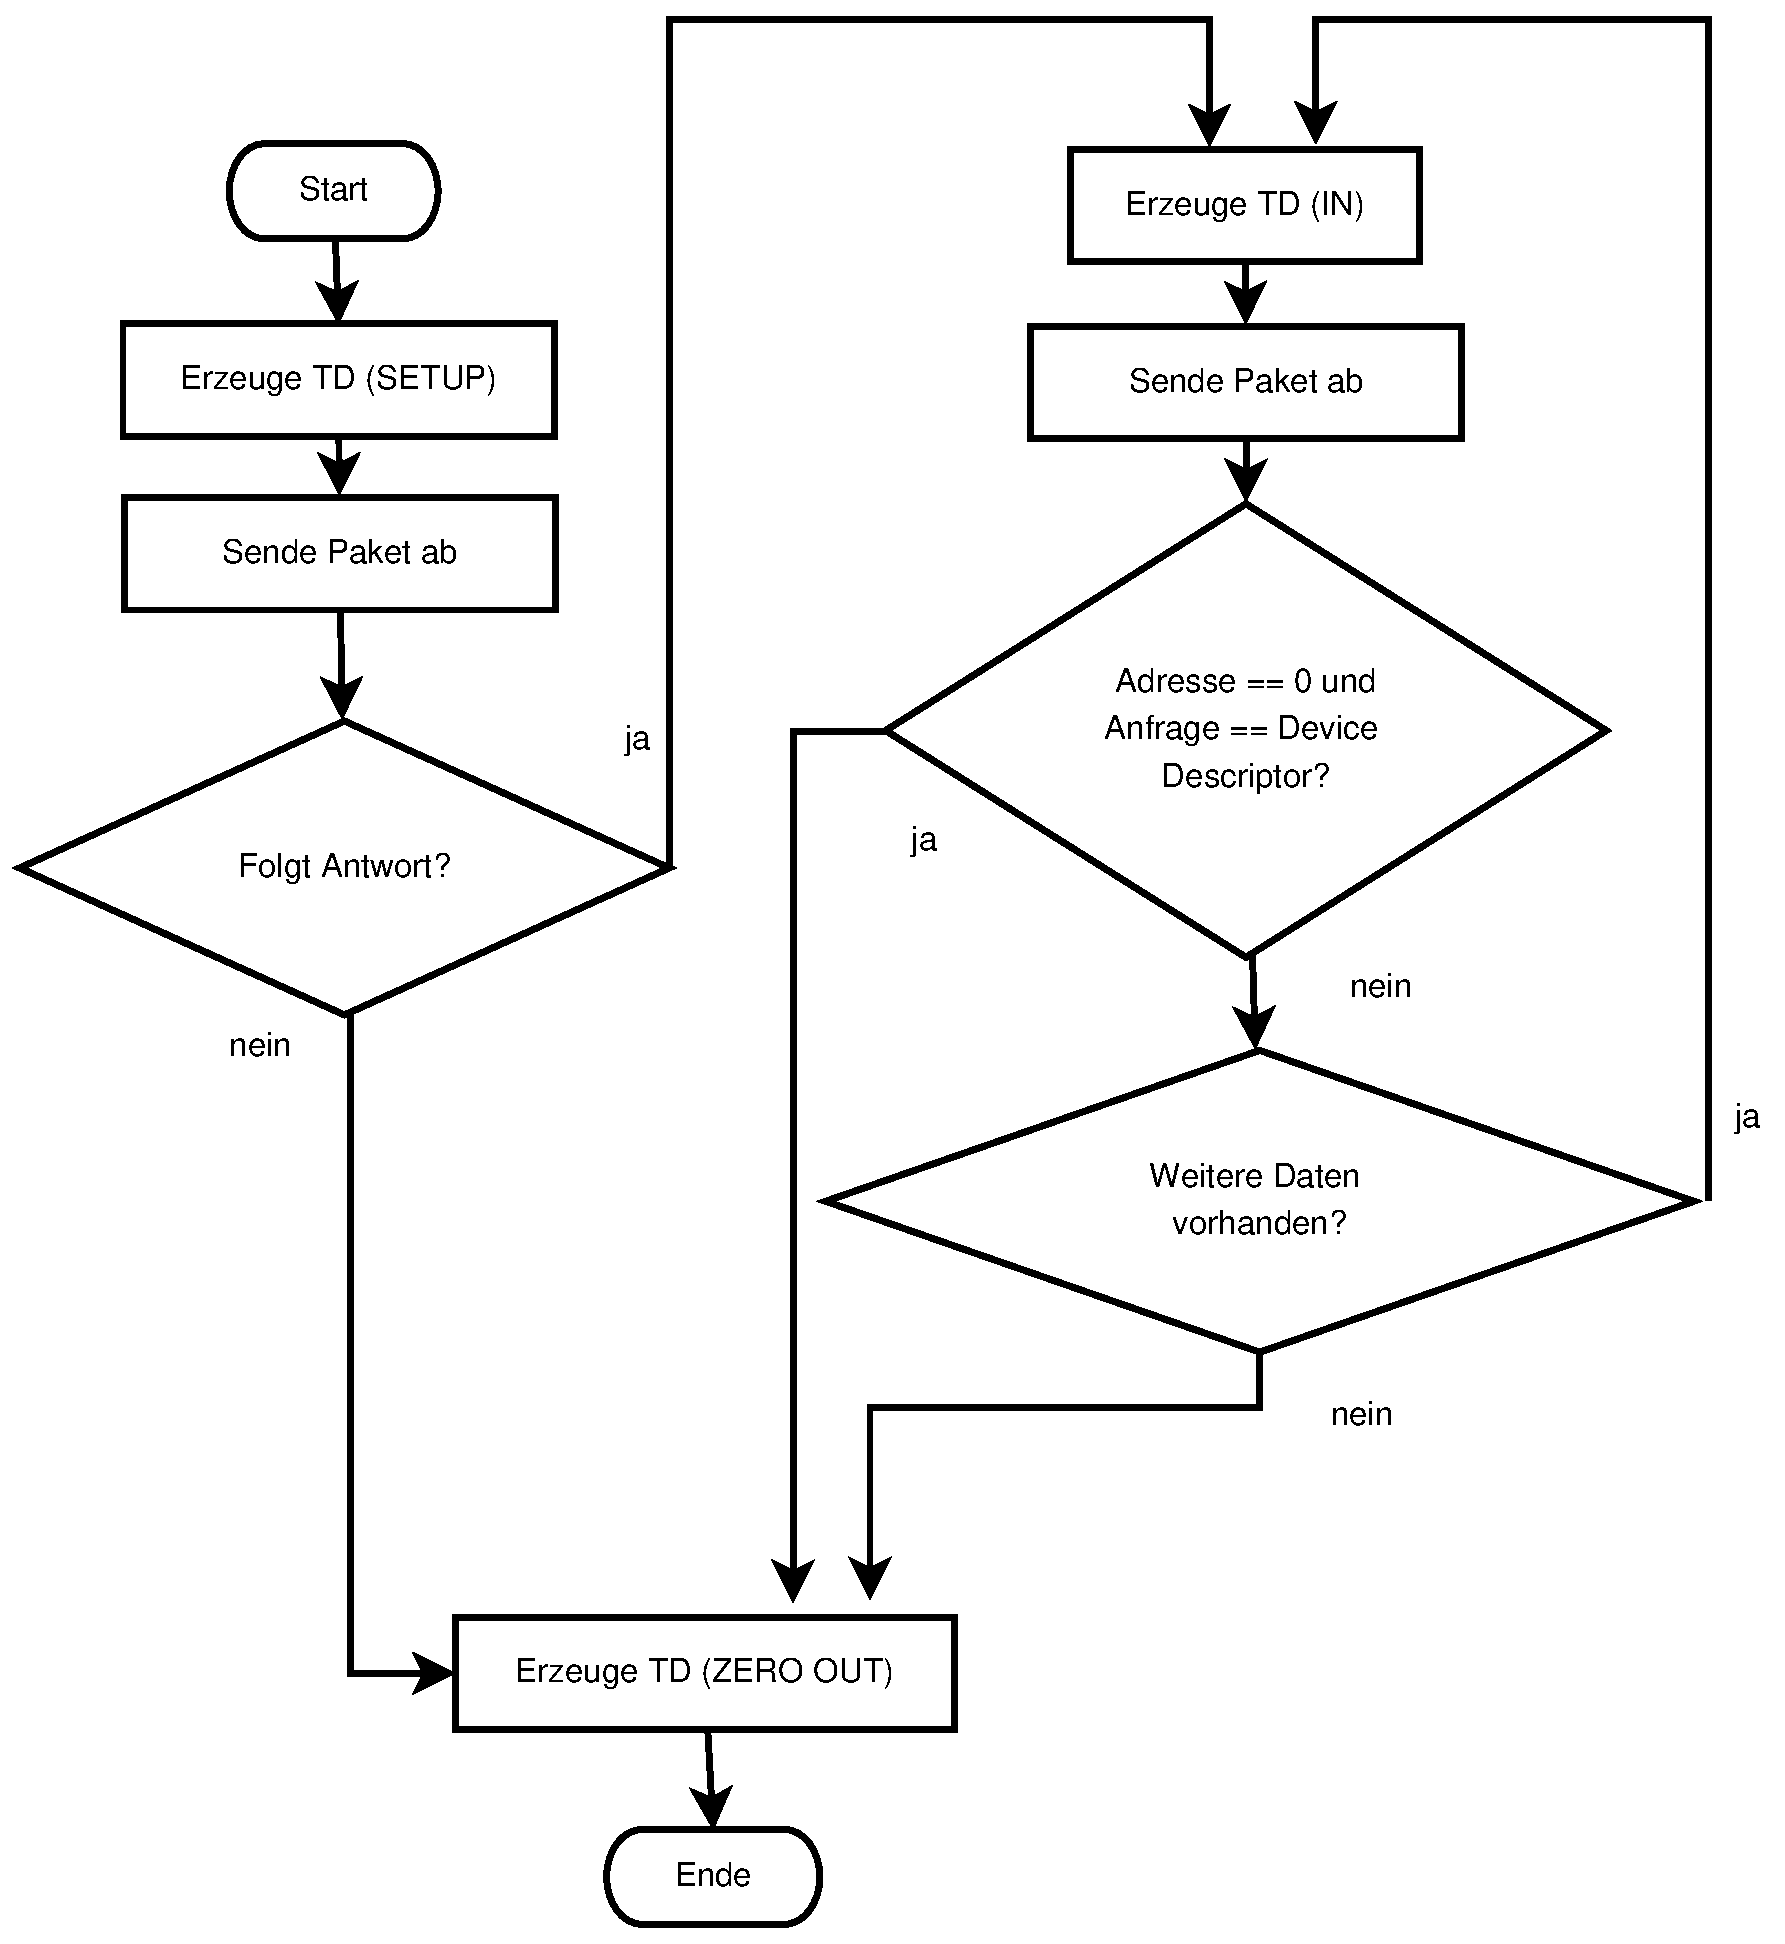
\includegraphics[width=12cm]{images/fluss_control}
\caption{Aufteilung eines Control-Transfers in Transfer-Deskriptoren}
\label{fluss_control}
}
\end{figure}




\section{Integration in ein eigenes Projekt}\label{integration}

Mit der folgenden Anleitung soll Schritt f�r Schritt
gezeigt werden, wie der USB-Stack in ein bestehendes oder
neues Projekt integriert werden kann. 
\newline\newline

\textbf{Schritt 1. USB-Verzeichnisse kopieren} \newline
\newline
Zu Beginn m�ssen die kompletten Verzeichnisse \textbf{core}, \textbf{lib} und \textbf{usbspec} aus dem USB-Stack-Archiv
in das eigene Projektverzeichnis kopiert werden. Wenn f�r den USB-Stack ein eigener
Unterordner erstellt werden soll, m�ssen die Verzeichnisse entsprechend in 
diesen Ordner kopiert werden.
\newline

\textbf{Schritt 2. Host-Treiber w�hlen} \newline
\newline
Im n�chsten Schritt muss ein Ordner \textbf{host} auf der gleichen Ebene des 
Ordners aus Schritt 1 angelegt werden. In diesen Ordner muss 
ein passender USB-Host-Controller-Treiber aus dem Archiv ausgew�hlt und dort hinkopiert werden. 
F�r die Compilierung wird dazu noch die Datei \textbf{host.h} gebraucht, daher muss diese
ebenfalls dorthin kopiert werden.
Oft ben�tigen die Treiber noch weitere Dateien, wie beispielsweise
im Fall des SL811HS-Treibers. Dort gibt es noch eine \textbf{sl811hs.h} Datei,
welche ebenfalls kopiert werden muss.
Wenn der Host-Controller nicht mit in den Mikroprozessor integriert ist,
muss ebenfalls noch die Verbindung und �bertragung zwischen Mikrocontroller und Host-Controller 
beschrieben werden. Daf�r bieten
die Host-Controller eigene Funktionen an, die allerdings angepasst werden m�ssen.
Wie die Anbindung genau erfolgt, muss den Dokumentationen der Host-Controller-Treiber
entnommen werden. F�r den SL811HS ist dies in Kapitel 8 der Diplomarbeit beschrieben.
\newline

\textbf{Schritt 3. Treiber und Bibliotheken w�hlen }\newline
\newline
Auf die selbe Weise wie der Host-Treiber m�ssen die ben�tigten Ger�tetreiber und Bibliotheken
in das erstellte Verzeichnis kopiert werden. Es ist zu empfehlen, die Verzeichnisstruktur genauso wie im USB-Stack-Archiv
aufzubauen.
\begin{itemize}
\item drivers 
  \begin{itemize}
    \item class  
    \item net
    \item ...
  \end{itemize}
\item uclibusb
\end{itemize}

Es exisitieren noch einige Ordner, die im USB-Stack-Archiv leer sind. Mit der Zeit wird
diese Sammlung hoffentlich immer gr��er werden.
\newline

\textbf{Schritt 4. Quelltexte in �bersetzungsprozess integrieren} \newline
\newline
Im n�chsten Schritt m�ssen die Dateien mit in den �bersetzungsprozess des Projektes eingebaut werden.
Damit der Compiler die ben�tigten Header-Dateien findet, muss
das Verzeichnis, in dem sich die USB-Stack-Dateien befinden, als Include-Pfad mitgegeben werden.
F�r den gcc w�rde der Aufruf \textit{gcc -I./}, oder wenn es einen extra Ordner f�r den
USB-Stack gibt, \textit{gcc -I./ordnerzumstack} hei�en. �ber das Pr�prozessor-Flag
DEBUG kann der Debugmodus ein- und ausgeschaltet werden (\textit{gcc -DDEBUG=1} oder \textit{gcc -DDEBUG=0}).
\newline

\textbf{Schritt 5. Inbetriebnahme des USB Stacks} \newline

Die wesentlichen Funktionsaufrufe werden am Listing \ref{lst:usb_sample} gezeigt.
In Zeile 1-4 sind die wichtigen Header-Dateien eingebunden. Welche
hier stehen m�ssen ist abh�ngig von den Treibern, die f�r die Anwendung
ben�tigt werden. Der USB Stack wird mit dem Funktionsaufruf
aus Zeile 8 initialisiert. Wieder abh�ngig von den ben�tigten Treibern
m�ssen die Initialisierungsfunktionen der Treiber aufgerufen werden (Zeile 10-11).
F�r Verwaltungs- und Steuerungsaufgaben muss der USB-Stack regelm��ig aufgerufen werden.
Dies kann entweder �ber eine Endlosschleife (Zeile 13) gel�st werden,
oder �ber einen periodischen Timer einer Thread-Bibliothek, etc.
Finden keine periodischen Transfers statt und werden USB-Ger�te nicht w�hrend
des Betriebs gewechselt, kann auf diesen periodischen Funktionsaufruf verzichtet werden.

\lstset{language=C}
\begin{lstlisting}[caption={Inbetriebnahme des USB-Stacks},label={lst:usb_sample},
captionpos=b,
numbers=left,
basicstyle=\ttfamily\fontsize{10}{12}\selectfont,
commentstyle=\fontsize{10}{12}\selectfont]
#include <core/core.h>
#include <host/host.h>
#include <drivers/class/hub.h>
#include <drivers/class/storage.h>

int main(void)
{
  usb_init();

  usb_hub_init();
  usb_storage_init();
  
  while(1){
    usb_periodic(); 
    wait_ms(1);
  }
  return 0;
}
\end{lstlisting}

\textbf{Schritt 6.  USB-Programme schreiben} \newline
Die Grundlagen sind an dieser Stelle geschaffen und es kann mit dem Programmieren
der USB-Anwendung begonnen werden. Eine Kommunikation mit einem USB-Ger�t,
das direkt mit den Funktionen des USBDI angesteuert werden kann, k�nnte wie folgt aussehen:

\lstset{language=C}
\begin{lstlisting}[caption={Beispiel f�r ein USB-Programm},label={lst:usb_driver_999},
captionpos=b,
numbers=left,
basicstyle=\ttfamily\fontsize{10}{12}\selectfont,
commentstyle=\fontsize{10}{12}\selectfont]
/* Zeiger auf Ger�tedatenstruktur */
usb_device * dev = NULL;
char buf[] = {'A','B','C'};

/* USB-Verbindung zum Ger�t �ffnen */
dev = usb_open(0x1234,0x5678);

/* Daten an Endpunkt senden */
usb_bulk_write(dev,2,buf,3,1000);

/* Daten vom Endpunkt lesen */
usb_bulk_read(dev,1,buf,3,1000);

/* Verbindung beenden */
usb_close(dev);

\end{lstlisting}
\index{Beispielprogramm}

%\section{Portierung auf eine neue Architektur}

%datentypen

%port leitungen fuer die hostcontroller treiber



%\section{USB Debug Monitor}
%\subsection{Integration in USB Host Stack}
%\subsection{Datenverkehr aufzeichnen}



	\chapter{Implementierung des USB-Host-Controller-Treibers f�r den SL811HS}

Ziel dieses Kapitels ist es, den Entwurfsprozess eines Host-Treibers
anhand des eingesetzten Bausteins SL811HS zu erl�utern.

\section{Der Baustein SL811HS}

\index{SL811HS}
Die Struktur und die technischen Daten �ber den SL811HS k�nnen 
in Kapitel \ref{kap:sl811} auf Seite \pageref{kap:sl811} nachgelesen werden.
In diesem Abschnitt werden die Details, 
die f�r die Programmierung des Treibers wichtig sind, angesprochen.

\subsubsection{Interrupt-Controller}

Der SL811HS \index{SL811HS} Interrupt-Controller verf�gt �ber eine
nach au�en gef�hrte Interrupt-Leitung (INTRQ), die bei verschiedenen
Ereignissen �ber interne Register aktiviert werden kann.
�ber ein Statusregister kann ermittelt werden, welche
Ereignisse ausgel�st worden sind.
Das Statusregister kann zur�ckgesetzt werden,
indem ein schreibender Zugriff auf das Register
ausgef�hrt wird.

\subsubsection{Speicher- und Register�bersicht}

Der SL811HS enth�lt 256 Bytes internen Speicher (siehe Abbildung \ref{sl811hs_ram}) f�r
den USB-Datenspeicher und die Control- bzw. Statusregister.
Im Host-Modus werden die ersten 16 Byte als Register
und die restlichen 240 Byte f�r die USB-Daten�bertragung
genutzt. Angesprochen wird der Speicher direkt
�ber die 8-Bit breite Busschnittstelle.

\begin{figure}[h]
{
\centering
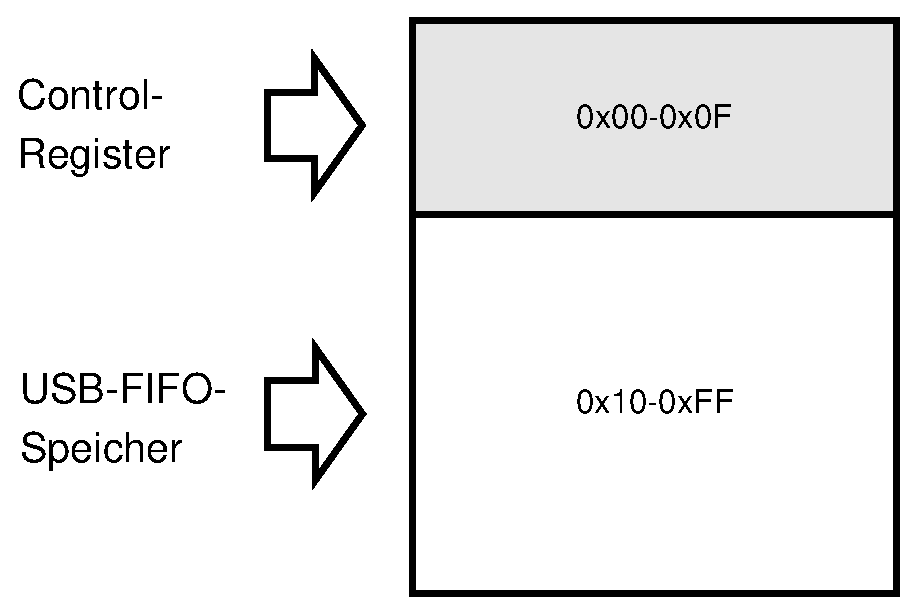
\includegraphics[width=5cm]{images/sl811hs_ram}
\caption{Speicherkarte des SL811HS}
\label{sl811hs_ram}
}
\end{figure}

\section{Anbindung an einen Mikrocontroller}

Um den Treiber flexibel und unabh�ngig von den verbundenen I/O Leitungen an den verschiedensten Mikrocontrollern
einsetzen zu k�nnen,
wurde eine extra Ebene (siehe Abbildung \ref{sl811hs_io}) daf�r eingef�hrt. 
Die Funktionen (siehe Tabelle \ref{sl811hs_func}) der zus�tzlichen Ebene
befinden sich in den Dateien \textbf{sl811hs-io.c} und \textbf{sl811hs-io.h},
welche 
sich absichtlich nicht im Host-Ordner, sondern in dem Ordner
der Anwendung, die den Stack nutzt, befinden.
Die Konfiguration ist von der Anwendung und der Plattform, auf der entwickelt wird, abh�ngig.

\begin{figure}[h]
{
\centering
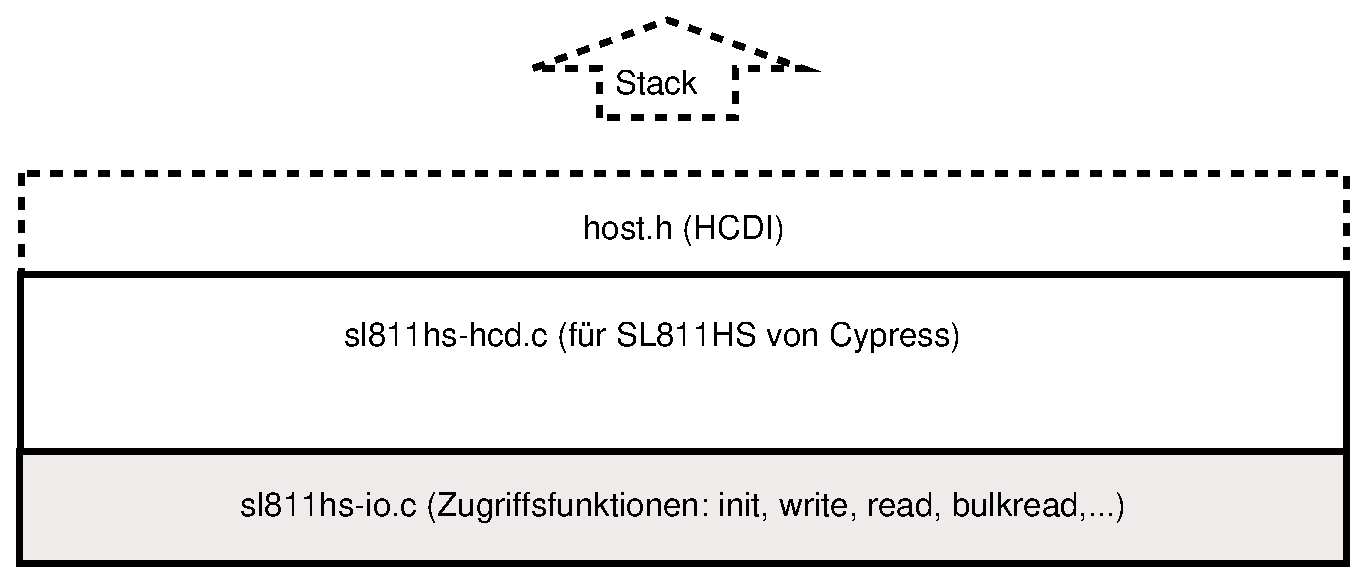
\includegraphics[width=10cm]{images/sl811hs_io}
\caption{Zugriffsfunktionen f�r SL811HS}
\label{sl811hs_io}
}
\end{figure}

\begin{table}[h]
\center
\begin{tabular}{|l|l|}
\hline
\rowcolor{Gray}[0.9\tabcolsep]
Funktion & Aufgabe\\ \hline
void sl811\_init() & Initialisierung der I/O-Leitungen\\ \hline
void sl811\_reset() & Reset des SL811HS durchf�hren\\ \hline
void sl811\_write(u8 addr, u8 data) & Byte an angegebene Adresse schreiben\\ \hline
u8 sl811\_read(u8 addr) & Byte an angegebener Adresse lesen\\ \hline
void sl811\_write\_burst(u8 data) & Bytes hintereinander schreiben\\ \hline
u8 sl811\_read\_burst() & Bytes hintereinander lesen\\ \hline
void sl811\_write\_buf(u8 addr, char *buf, u16 size) & Speicherbereich schreiben\\ \hline
void sl811\_read\_buf(u8 addr, char *buf, u16 size) & Speicherbereich lesen\\ \hline
\end{tabular}
\caption{Zugriffsfunktionen f�r SL811HS [sl811hs-io.h]}
\label{sl811hs_func}
\end{table}
\index{Zugriffsfunktionen f�r SL811HS}
\newpage
\section{Root-Hub-Treiber} \label{kap:roothub}
\index{Root-Hub-Treiber}
Die Funktionen f�r den Root-Hub-Treiber befinden sich mit unter in der Datei \textit{sl811hs-hcd.c}.
In den folgenden Listings wird auf die Implementierung der Funktionen eingegangen.
Der komplette Quelltext befindet sich im Host-Verzeichnis des USB-Stack-Archivs.
\newline\newline
Bekannterma�en ist der Root-Hub kein eigenes physikalisches USB-Ger�t,
sondern eine feste Einheit im Host-Controller. Im Gegensatz zu einem
externen USB-Hub wird der Status �ber die angesteckten USB-Ger�te am Hub
nicht �ber Endpunkte signalisiert, sondern �ber interne Register und Signale.
Dies sind die Aufgaben der Funktionen des Root-Hub-Treibers. Es m�ssen
die entsprechenden Register und Signale beobachtet und
neue und entfernte Ger�te dem USB-Stack gemeldet werden. 
\newline\newline
Wie jeder Ger�te- bzw. Klassen-Treiber ben�tigt auch der Root-Hub eine USB-Treiberdatenstrukur,
um sich am USB-Stack registrieren zu k�nnen.
\vskip 10pt  
\lstset{language=C}
\begin{lstlisting}[caption={SL811-Host-Controller-Treiber, sl811hs-hcd.c},label={sl811hs_rh},
name=roothub,
captionpos=b,
numbers=left,
firstline=1,
basicstyle=\ttfamily\fontsize{10}{12}\selectfont,
commentstyle=\fontsize{10}{12}\selectfont]
/* Treiberdatenstruktur */
usb_driver sl811_roothub = {
  .name   = "sl811_roothub",
  .probe  = sl811_roothub_probe,
  .check  = sl811_roothub_check,
  .data   = NULL,
};
\end{lstlisting}
\vskip 10pt  
Die \textit{probe} Funktion eines Treibers wird jedesmal
vom USB-Stack aufgerufen, wenn ein neues Ger�t am Bus
gefunden worden ist. In ihr wird �berpr�ft, ob das neue Ger�t von dem Treiber aus
angesteuert werden kann. Der Root-Hub-Treiber muss
diese �berpr�fung nicht durchf�hren, da der Host-Controller
einen Schritt zuvor schon ermittelt hat, ob der SL811-Baustein
verf�gbar ist. Ist dies der Fall, so ist
der Root-Hub ebenso verf�gbar, da er wie bereits beschrieben
eine feste Einheit im Host-Controller ist. Daher kann 
die Funktion \textit{sl811\_roothub\_probe} leer bleiben.
\vskip 10pt  
\begin{lstlisting}[caption={sl811\_roothub\_probe(), sl811hs-hcd.c},label={sl811hs_rh},
captionpos=b,
numbers=left,
name=roothub,
basicstyle=\ttfamily\fontsize{10}{12}\selectfont,
commentstyle=\fontsize{10}{12}\selectfont]
void sl811_roothub_probe()
{
  /* Root-Hub wurde bereits vom Host-Controller-Treiber erkannt */
}
\end{lstlisting}
\vskip 10pt  

Die �berwachung des abgehenden Ports am SL811-Host-Controller
wird in der Funktion \textit{sl811\_roothub\_check} vollzogen.
Die Funktionsweise wurde einem echten USB-Hub nachempfunden.
Bei einem USB-Hub existieren im Wesentlichen zwei Register. Im Ersten wird
der aktuelle Status angezeigt, d.h. ob sich im Moment ein Ger�t
an einem Port befindet. Im Zweiten ist ersichtlich,
ob ein Ger�t entfernt oder neu angesteckt wurde.
Mit Hilfe der Variable \textit{port\_change},
wird das Register f�r die �nderungen an dem Port nachgebildet.
Der Funktionsaufruf aus Zeile 19 entspricht dem ersten Register,
da hier der aktuelle Status des Ports abgefragt wird.


\vskip 10pt  
\begin{lstlisting}[caption={sl811\_roothub\_check(), sl811hs-hcd.c},label={sl811hs_rh},
captionpos=b,
numbers=left,
name=roothub,
showstringspaces=false,
basicstyle=\ttfamily\fontsize{10}{12}\selectfont,
commentstyle=\fontsize{10}{12}\selectfont]
void sl811_roothub_check()
{
  /* Ports �berwachen */
  // check for new device
  u16 *port_change = (u16*)sl811_roothub.data;

  // Status des Ports abfragen
  u8 status = sl811_read(SL811_ISR);
  // Signale zur�cksetzten
  sl811_write(SL811_ISR,SL811_ISR_DATA | SL811_ISR_SOFTIMER);

  // Entferne Ger�t gegebenenfalls
  if((status & SL811_ISR_RESET)) {  
    if(device_on_downstream!=NULL){
      #if USBMON
      core.stdout("Remove Device!\r\n");
      #endif
      usb_remove_device(device_on_downstream);
      device_on_downstream=NULL;
    }
    sl811_write(SL811_ISR,SL811_ISR_RESET);
  } 
\end{lstlisting}
\vskip 10pt  

Meldet der Root-Hub ein neues Ger�t, so 
wird der Port f�r den USB-Betrieb konfiguriert.
Es wird unteranderem die Generierung der SOF-Pakete
gestartet, das Ger�t mit Hilfe des Resetsignals
dazu veranlasst die Adresse 0 anzunehmen 
und zum Schluss die Enumerierung f�r das
USB-Ger�t gestartet. Mit dem Aufruf der
Funktion \textit{usb\_add\_device} aus Zeile 56
wird das neue Ger�t desweiteren am USB-Stack angemeldet.
\vskip 10pt  
\begin{lstlisting}[caption={Root-Hub Funktionalit�t, sl811hs-hcd.c},label={sl811hs_rh},
captionpos=b,
numbers=left,
name=roothub,
showstringspaces=false,
basicstyle=\ttfamily\fontsize{10}{12}\selectfont,
commentstyle=\fontsize{10}{12}\selectfont]
  else {
    if((port_change[0] & HUB_PORTSTATUS_C_PORT_CONNECTION)){
      #if USBMON
      core.stdout("Find new Device!\r\n");
      #endif

      /* init sof currently for fullspeed  (datasheet page 11)*/
      sl811_write(SL811_CSOF,0xAE);
      sl811_write(SL811_DATA,0xE0);

      /* reset device that function can answer to address 0 */
      sl811_write(SL811_IER,0x00);
      sl811_write(SL811_CTRL,SL811_CTRL_ENABLESOF|SL811_CTRL_RESETENGINE);
      sl811_write(SL811_ISR,0xff);
      wait_ms(20);

      /* start SOF generation */
      sl811_write(SL811_CTRL,SL811_CTRL_ENABLESOF);
      sl811_write(SL811_ISR,0xff);
      sl811_write(SL811_E0BASE,SL811_EPCTRL_ARM);
      wait_ms(50);

      device_on_downstream = usb_add_device();
      port_change[0]=0x00;
    }
  }
\end{lstlisting}
\vskip 10pt  

In den Zeilen 60-63 wird die Variable \textit{port\_change} f�r die �nderungen
abh�ngig vom abgefragten Ergebnis der Register des SL811HS
neu gesetzt.

\vskip 10pt  
\begin{lstlisting}[caption={port\_change, sl811hs-hcd.c},label={sl811hs_rh},
captionpos=b,
numbers=left,
name=roothub,
basicstyle=\ttfamily\fontsize{10}{12}\selectfont,
commentstyle=\fontsize{10}{12}\selectfont]
  if((status & SL811_ISR_INSERT)){
    port_change[0] |= HUB_PORTSTATUS_C_PORT_CONNECTION;
    sl811_write(SL811_ISR,SL811_ISR_INSERT);
  }
}
\end{lstlisting}
\vskip 10pt  


\section{Transfer-Deskriptoren-�bertragungsstrategie}
\index{Transfer-Deskriptor}


Der SL811HS bietet alle Control- und Statusregister (siehe Tabelle \ref{sl811hs_register} auf Seite \pageref{sl811hs_register}) f�r
die �bertragung von USB-Paketen doppelt (Registerset A und B) an.
Dadurch kann die Bandbreite der USB-Verbindung
besser genutzt werden. Ist eine Transaktion
abgeschlossen wird �ber das Interruptstatusregister angezeigt,
welches Registerset wieder bereit f�r ein neues Paket ist.
\newline\newline
Im folgenden wird auf den Quelltext der Funktion \textit{sl811\_start\_transfer} eingegangen,
welche f�r die �bertragung der einzelnen Transfer-Deskriptoren zust�ndig ist.
Im Rahmen der Diplomarbeit wurde eine einfache Version ausgearbeitet,
in der nur ein Registerset ohne Interruptbetrieb genutzt wird. Dieser 
Modus wird auch Bibliotheksmodus (\glqq{}LIBMODE\grqq{}) genannt,
da man so den USB-Stack wie eine einfache Funktionssammlung nutzen
kann, ohne ihn fester in die eigene Anwendung integrieren zu m�ssen.
\newline\newline
Beginnend wird in Zeile 3 ein Zeiger auf einen Transferdeskriptor erstellt,
mit dem im weiteren Verlauf der Funktion gearbeitet werden kann.
In Zeile 6 erh�lt der Zeiger die Adresse auf den n�chsten zu �bertragende Transferdeskriptor. 
\vskip 10pt  
\begin{lstlisting}[caption={SL811 �bertragungsfunktion f�r Transferdeskriporen, sl811hs-hcd.c},label={sl811hs_td},
captionpos=b,
numbers=left,
name=transfer,
basicstyle=\ttfamily\fontsize{10}{12}\selectfont,
commentstyle=\fontsize{10}{12}\selectfont]
void sl811_start_transfer()
{
  usb_transfer_descriptor * td;
  #if LIBMODE
  /* W�hle n�chsten Transferdeskriptor */
  td = td_usba;
  /* Interruptsignale abschalten (im LIBMODUS) */
  sl811_write(SL811_IER,0x00);
  #endif
\end{lstlisting}
\vskip 10pt  
Unabh�ngig vom Pakettyp, welcher im Transferdeskriptor angegeben ist,  muss f�r die �bertragung die
Adresse des USB-Ger�tes, die Anzahl der zu �bertragenden
Bytes und die Startadresse der Daten angegeben werden.
\vskip 10pt  
\begin{lstlisting}[caption={Transfer unah�ngige Einstellungen},label={sl811hs_td},
captionpos=b,
numbers=left,
name=transfer,
basicstyle=\ttfamily\fontsize{10}{12}\selectfont,
commentstyle=\fontsize{10}{12}\selectfont]
  sl811_write(SL811_E0CONT,td->devaddress); /* Ger�teadresse */
  sl811_write(SL811_E0LEN,td->actlen);      /* Anzahl der Bytes */
  sl811_write(SL811_E0ADDR,cMemStart);      /* Adresse f�r Daten */
\end{lstlisting}
\vskip 10pt  
Im folgenden muss abh�ngig vom Pakettyp unterschiedlich vorgegangen werden.
Differenziert wird hier zwischen SETUP-, IN- und OUT-Paket. Wobei Daten
immer nach einem IN oder OUT Paket folgen. Handelt es sich um ein SETUP-Paket,
wird zuerst die Anfrage (Standard-, Hersteller- oder Klassenanfrage) in
den internen Speicher des SL811HS-Host-Controllers kopiert (Zeile 17).
In Zeile 20 und 23 wird der Paket-Typ, die Endpunktnummer und der Datenpakettyp
dem Host-Controller mitgeteilt. Anschliessend wird der Transfer gestartet
und der Transferdeskriptor als versendet markiert.
\vskip 10pt  
\begin{lstlisting}[caption={PID-Setup, sl811hs-hcd.c},label={sl811hs_td},
captionpos=b,
numbers=left,
name=transfer,
basicstyle=\ttfamily\fontsize{10}{12}\selectfont,
commentstyle=\fontsize{10}{12}\selectfont]
  switch(td->pid) {
    case USB_PID_SETUP:

      /* Kopiere Anfrage in internen SL811HS RAM */
      sl811_write_buf(cMemStart,(unsigned char *)td->buffer,td->actlen);

      /* set pid and ep */
      sl811_write(SL811_E0STAT,PID_SETUP|td->endpoint); 

      /* Sende Setup-Paket mit DATA0 */
      sl811_write(SL811_E0CTRL,DATA0_WR); 

      /* Warte auf ACK */
      #if LIBMODE
      while((sl811_read(SL811_ISR)&SL811_ISR_USBA)==0);
      #endif
      td->state = USB_TRANSFER_DESCR_SEND;

    break;
\end{lstlisting}
\vskip 10pt  
Werden Daten von einem USB-Ger�t empfangen, m�ssen IN-Pakete versendet werden.
Als Antwort auf ein IN-Paket erh�lt der Host-Controller die Daten vom USB-Ger�t.
In Zeile 35 wird dem Host-Controller der Pakettyp und die Endpunktadresse mitgeteilt.
Zus�tzlich muss das Togl-Bit entsprechend gesetzt werden, um den Datenfluss
zu erm�glichen.
\vskip 10pt  
\begin{lstlisting}[caption={PID-IN, sl811hs-hcd.c},label={sl811hs_td},
captionpos=b,
numbers=left,
name=transfer,
basicstyle=\ttfamily\fontsize{10}{12}\selectfont,
commentstyle=\fontsize{10}{12}\selectfont]
    case USB_PID_IN:
      
      /* Pakettyp und Endpunkt setzten */
      sl811_write(SL811_E0STAT,PID_IN|td->endpoint); 
      sl811_write(SL811_ISR,0xff);

      /* DATA0 oder DATA1 */
      if(td->togl)
	sl811_write(SL811_E0CTRL,DATA1_RD); 
      else
	sl811_write(SL811_E0CTRL,DATA0_RD);

      td->state = USB_TRANSFER_DESCR_SEND;

      /* Warte auf ACK */
      #if LIBMODE
      while((sl811_read(SL811_ISR)&SL811_ISR_USBA)==0);

      /* Empfangene Daten vom internen SL811HS-RAM lesen */
      sl811_read_buf(cMemStart,(unsigned char *)td->buffer,td->actlen);
      #endif

    break;
\end{lstlisting}
\vskip 10pt  
Ausgehende Daten werden mit OUT-Paketen an USB-Ger�te gesendet.
Der Ablauf zu den anderen Pakettypen unterscheidet
sich nur darin, dass zuvor die zu �bertragenden Daten
in den internen Speicher des SL811HS geschrieben werden m�ssen.
\vskip 10pt  
\begin{lstlisting}[caption={PID-OUT, sl811hs-hcd.c},label={sl811hs_td},
captionpos=b,
numbers=left,
name=transfer,
basicstyle=\ttfamily\fontsize{10}{12}\selectfont,
commentstyle=\fontsize{10}{12}\selectfont]
    case USB_PID_OUT:
      /* Schreibe zu �bertragende Daten in SL811HS-RAM */
      if(td->actlen>0)
	sl811_write_buf(cMemStart,(unsigned char *)td->buffer,td->actlen);
     
      /* Pakettyp und Endpunktadresse */
      sl811_write(SL811_E0STAT,PID_OUT|td->endpoint);
      
      /* DATA0 oder DATA1 */
      if(td->togl)
	sl811_write(SL811_E0CTRL,DATA1_WR);
      else
	sl811_write(SL811_E0CTRL,DATA0_WR);

      td->state = USB_TRANSFER_DESCR_SEND;

      /* Warte auf ACK */
      #if LIBMODE
      while((sl811_read(SL811_ISR)&SL811_ISR_USBA)==0);
      #endif
    break;
  }    
}
\end{lstlisting}

\begin{table}[h]
\center
\begin{tabular}{|c|l|l|}
\hline
\rowcolor{Gray}[0.9\tabcolsep]
Adr. & Schreibzugriff & Lesezugriff\\ \hline\hline
0x00 & USB-A Control & USB-A Control\\ \hline
0x01 & USB-A Address & USB-A Address\\ \hline
0x02 & USB-A Length & USB-A Length\\ \hline
0x03 & USB-A PID/EP & USB-A Status\\ \hline
0x04 & USB-A Address & USB-A Count\\ \hline\hline
0x05 & Ctrl1 & Ctrl1\\ \hline
0x06 & Int. Enable & Int. Enable\\ \hline\hline
0x08 & USB-B Control & USB-B Control\\ \hline
0x09 & USB-B Address & USB-B Address\\ \hline
0x0A & USB-B Length & USB-B Length\\ \hline
0x0B & USB-B PID/EP & USB-B Status\\ \hline
0x0C & USB-B Address & USB-B Count\\ \hline\hline
0x0D & Int. Status & Int. Status \\ \hline
0x0E & SOF Low & HW Revision \\ \hline
0x0F & SOF High/Ctr2  & SOF High/Ctr2 \\ \hline
\end{tabular}
\caption{SL811HS Register�bersicht}
\label{sl811hs_register}
\end{table}


	\chapter{Implementierung der USB-Bibliotheken und -Ger�tetreiber}

Die wichtigsten Komponenten des USB-Stacks sind die Treiber und Bibliotheken der USB-Ger�te.
Mit ihnen kann eine abstrahierte Schnittstelle
f�r die Funktionen der einzelnen Ger�te angeboten werden.
Da die Treiber und Bibliotheken mit den Funktionen des USB-Stacks arbeiten
und nicht direkt mit den Host-Controllern kommunizieren,
k�nnen diese unabh�ngig vom eingesetzten Host-Controller
verwendet werden.
\newline\newline
Wie bereits erw�hnt, gibt es zwei Arten f�r die Ansteuerung 
eines USB-Ger�ts, Bibliotheken oder Treiber. Bibliotheken bieten sich vor allem f�r 
einfache Ger�te an, die �ber keine periodischen Endpunkte (wie Interrupt und Isochrone)
verf�gen. Soll ein USB-Ger�t hingegen von mehreren parallelen 
Programmpfaden aus angesprochen werden, so ist die Wahl eines Treibers die bessere M�glichkeit.
Der Treiber,
der die Zugriffszeiten gerecht auf alle Prozesse verteilen kann, dient als Schnittstelle zum Ger�t.
Abh�ngig vom Ger�t kann in den Treibern eigens der Mehrfachzugriff gesteuert werden.
\newline\newline
In den Treibern und Bibliotheken werden f�r die Kommunikation
und Steuerung der Verbindung die Funktionen des USB-Stacks verwendet (siehe Kapitel \ref{kap:usbdi} auf Seite \pageref{kap:usbdi}).
\newline\newline
Im n�chsten Abschnitt wird die Funktionsweise einer USB-Ger�te-Bibliothek erkl�rt.

\section{Bibliotheken} \label{kap:bib}
\index{Bibliotheken}
Der gro�e Vorteil von Bibliotheken gegen�ber Treibern ist,
dass sie leicht in den Programmfluss eines Programms
integriert werden k�nnen. An der Stelle, an der die Information 
vom USB Ger�t ben�tigt wird, muss die daf�r vorgesehene Bibliotheksfunktion einfach eingef�gt werden.
Sobald die Funktion das Ergebnis ermittelt hat, setzt das Hauptprogramm
mit der Arbeit fort. Der Nachteil von Bibliotheken ist, dass kostbare Rechenzeit
beim Warten auf das Ergebnis verloren geht. Oft kann dies 
aber f�r die Einfachheit in Kauf genommen werden, falls die Rechenzeit nicht anderweitig ben�tigt wird.
\newline\newline
Um eine Kommunikation mit einer Bibliothek durchf�hren zu k�nnen,
muss erst ein \glqq{}Handle\grqq{}\footnote{\label{foot:usbdi}\glqq{}Handle\grqq{} werden in der Informatik meist Zeiger auf Dateien oder Ger�te genannt.} f�r das Ger�t
erstellt werden. Im USB-Stack ist ein Handle ein Zeiger auf die \textit{usb\_device} Struktur (siehe Listing \ref{lst:usb_dev_struct} auf Seite \pageref{lst:usb_dev_struct})
des ausgew�hlten Ger�tes. Das Handle kann auf drei verschiedene Arten angelegt werden.

\begin{enumerate}
\item Mit der Funktion \textit{usb\_open} kann das Ger�t �ber die Hersteller- und Produkt-ID gefunden werden.
\item �ber den Klassencode kann das Ger�t mit der Funktion \textit{usb\_open\_class} gefunden werden.
\item Werden spezielle Deskriptoren f�r die Auswahl des Ger�tes ben�tigt, so kann ebenso �ber die interne Ger�teliste des USB-Kerns iteriert
und entsprechend f�r jedes Ger�t die spezielle Information abgefragt werden.
\end{enumerate}

Hat man den Zeiger auf das gesuchte Ger�t erhalten, kann mit den Funktionen 
einer Bibliothek gearbeitet werden. 
\newline\newline
Im folgenden wird eine Bibliothek vorgestellt, die im Rahmen der Diplomarbeit entstanden ist.
Die Bibliotheken befinden sich im Ordner uclibusb des Softwarearchivs.

\subsection{USB zu RS232-Wandler: FT232}
\index{FT232}
\index{RS232}
\index{USB zu RS232-Wandler}
\subsubsection{Struktur und Arbeitsweise}
Der FT232AM bzw. dessen Nachfolger der FT232BM von FTDI ist
ein Umsetzer von USB-zu-TTL-RS232-Signalen. F�r die Leitung RX und TX
gibt es jeweils einen Bulk-Endpunkt. Schreibt man in den TX-Endpunkt,
so werden die Daten �ber den UART des FT232 ausgegeben. Liest man im Gegensatz
von dem RX-Endpunkt, so erh�lt man die �ber den UART empfangenen Daten.
Intern, wie in Abbildung \ref{ftdi} zu sehen ist, sind direkt nach den UART
Leitungen TX und RX kleine FIFOs als Zwischenpuffer f�r die
empfangenen und zu sendenden Daten vorhanden.

\begin{figure}[h]
{
\centering
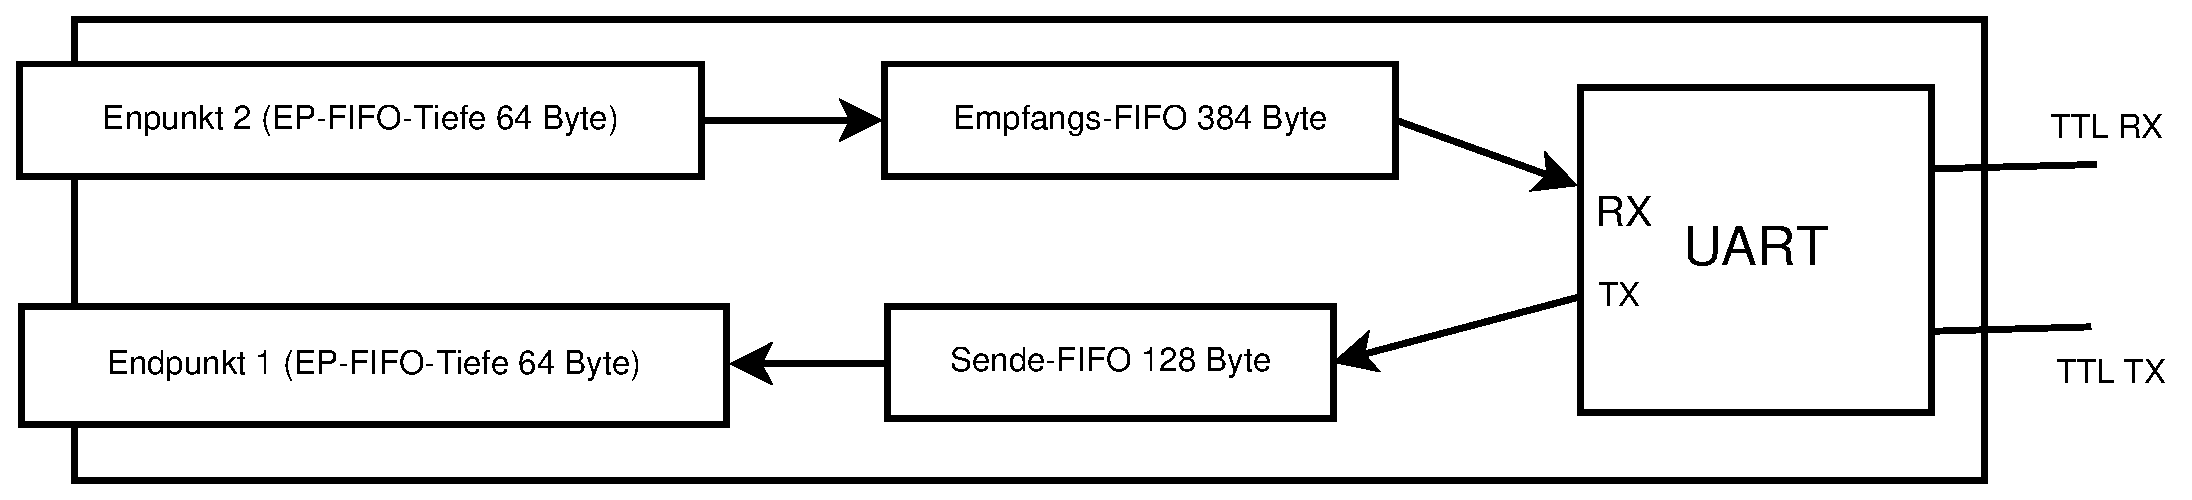
\includegraphics[width=15cm]{images/ftdi}
\caption{FT232-Struktur}
\label{ftdi}
}
\end{figure}

\newpage
\subsubsection{Konfiguration}

Der Hersteller FTDI bietet f�r die Konfiguration des Ger�tes
verschiedene Herstelleranfragen (engl. \glqq{}Vendor Requests\grqq{}, siehe Kapitel 2.15) an.
In Tabelle \ref{usb_ftdi} ist eine �bersicht der verschiedenen Anfragen dargestellt.

\begin{table}[h]
\center
\begin{tabular}{|l|l|l|}
\hline
\rowcolor{Gray}[0.9\tabcolsep]
Anfrage & Nr.& Beschreibung \\ \hline
FTDI\_SIO\_RESET  &0& L�st ein Reset des Ports aus \\ \hline
FTDI\_SIO\_MODEM\_CTRL &1& Modem-Controllregister beschreiben \\ \hline
FTDI\_SIO\_SET\_FLOW\_CTRL &2& Flusscontrollregister beschreiben\\ \hline
FTDI\_SIO\_SET\_BAUD\_RATE &3& �bertragungsrate einstellen\\ \hline
FTDI\_SIO\_SET\_DATA &4& Die Eigenschaft des Ports definieren\\ \hline
FTDI\_SIO\_GET\_MODEM\_STATUS &5& Abfrage des Modem-Status-Registers \\ \hline
FTDI\_SIO\_SET\_EVENT\_CHAR &6& Steuerzeichen definieren\\ \hline
FTDI\_SIO\_SET\_ERROR\_CHAR &7& Fehlerzeichen definieren\\ \hline
FTDI\_SIO\_SET\_LATENCY\_TIMER &8& Latenzzeit einstellen\\ \hline
FTDI\_SIO\_GET\_LATENCY\_TIMER &9& Latenzzeit abfragen\\ \hline
\end{tabular}
\caption{Herstelleranfragen des FT232}
\label{usb_ftdi}
\end{table}
Die Anfragen werden auf die gleiche Weise wie Standardanfragen �ber den Endpunkt 0
an das Ger�t gesendet. Da es vom Hersteller FDTI keine �bersicht
der einzelnen Nachrichten gibt, wurden die Parameter dem
offenen Linux-Treiber ftdi\_sio.c \cite{kernel} entnommen.

\subsubsection{Bibliotheksfunktionen}
\begin{table}[h]
\center
\begin{tabular}{|l|l|}
\hline
\rowcolor{Gray}[0.9\tabcolsep]
Anfrage & Beschreibung \\ \hline
\text{usb\_device * usb\_ft232\_open()} &  �ffnen der Verbindung \\ \hline
\text{usb\_ft232\_close(usb\_device *dev)} &  Beenden der Verbindung \\ \hline
\text{usb\_ft232\_send(usb\_device *dev,char *bytes, u8 length)} &  Daten senden \\ \hline
\text{usb\_ft232\_receive(usb\_device *dev,char *bytes, u8 length)} &  Daten  empfangen\\ \hline
\end{tabular}
\caption{Bibliotheksfunktionen des FT232, ft232.h}
\label{usb_ftdi_api}
\end{table}

Befindet sich ein FT232-Baustein am Bus des USB-Stacks,
so kann mit der Funktion \textit{usb\_ft232\_open} das Handle
f�r eine Kommunikation geholt werden. Um Daten versenden zu k�nnen,
existiert die Funktion \textit{usb\_ft232\_send}, um Daten entsprechend
empfangen zu k�nnen die Funktion \textit{usb\_ft232\_receive}. Als Parameter erwarten
beide Funktionen einen Zeiger auf die Ger�tedatenstruktur des angeschlossenen FT232-Bausteins, einen Zeiger auf einen Speicherbereich,
der zum Versenden oder zum Empfangen reserviert ist und als letzter Parameter wird die Anzahl der zu sendenden 
oder zu empfangenden Daten erwartet. Wird das Ger�t f�r die Kommunikation nicht 
mehr ben�tigt, kann das Ger�t mit \textit{usb\_ft232\_close} wieder
freigegeben werden.



\section{Ger�te- und Klassentreiber}
\index{Ger�tetreiber}
\index{Klassentreiber}
\subsection{Treiberarten}
F�r USB-Ger�te gibt es zwei Treiberarten, die Ger�tetreiber
und die Klassentreiber. Ein Ger�tetreiber ist speziell
f�r eine bestimmte Hardware entwickelt worden. Kauft man ein solches Ger�t,
so muss der dazugeh�rige vom Hersteller mitgelieferte Treiber installiert werden.
\newline\newline
F�r Standardger�te wie M�use, Tastaturen, Drucker, Netzwerkkarten, etc.
wurden mit der USB-Spezifikation sogenannte USB-Klassen definiert.
Eine Klasse beschreibt eine Schnittstellenstruktur f�r
eine bestimmte Ger�teklasse. Das Ziel dieser Klassen ist,
dass auf dem Rechner keine speziellen Treiber mehr f�r
Standardger�te installiert werden m�ssen. Dies bedeutet
aber nicht, dass diese Ger�te keine Treiber mehr ben�tigen.
Die Betriebssysteme halten Standardtreiber daf�r vor.
Daher entf�llt die Installation f�r den Benutzer und
Hersteller von Standardperipherie m�ssen keine Treiber mehr entwickeln und
verteilen.
\newline\newline
Die bekanntesten Ger�teklassen werden in einzelnen Dokumenten
von der USB-Organisation beschrieben:
\index{Human-Interface-Devices}
\index{Audio-Device-Class}
\index{Communication-Class-Device}
\index{Mass-Storage-Device-Class}
\index{Printer-Device-Class}
\begin{itemize}
\item Human-Interface-Devices \cite{class_hid}
\item Audio-Device-Class \cite{class_audio}
\item Communication-Class-Device \cite{class_cdc}
\item Mass-Storage-Device-Class \cite{class_msd}
\item Printer-Device-Class \cite{class_print}
\end{itemize}

\subsection{Automatische Treiberauswahl f�r Ger�te}
Wie in Kapitel \ref{kap:usbdi_driver} auf Seite \pageref{kap:usbdi_driver}
bereits angesprochen, werden Ger�te- und Klassentreiber
mit einer Instanz der Datenstruktur \textit{usb\_driver} (siehe Listing \ref{lst:usb_driver} auf Seite \pageref{lst:usb_driver}) am USB Stack registriert.
Die Datenstruktur enth�lt Zeiger auf die folgenden Funktionen eines Treibers.

\begin{description}
\item [usb\_$<$treibername$>$\_probe:] 
Diese Funktion wird immer dann vom USB-Stack aus aufgerufen, wenn ein neues Ger�t
am Bus erkannt wird. Sie �berpr�ft, ob das neue
Ger�t mit dem Treiber angesteuert werden kann. Dies kann
mit den gleichen drei M�glichkeiten wie f�r Bibliotheken aus Kapitel \ref{kap:bib} auf Seite \pageref{kap:bib} herausgefunden werden.
Ist das Ger�t von dem Treiber ansteuerbar, kann die Funktion das Ger�t in die internen Datenstrukturen 
des Treibers aufnehmen.
\newline\newline
F�r die Klassentreiber gibt es extra Felder im Ger�te- und Interface-Deskriptor des USB-Ger�tes,
in denen ein Klassencode angegeben werden kann. Mit speziellen Unterklassencodes
und Protokollnummern kann das Ger�t noch genauer identifiziert werden.

\item [usb\_$<$treibername$>$\_check:]
Befindet sich mindestens ein aktives Ger�t in den internen Treiberdatenstrukturen,
so wird im regelm��igen Abstand von einer Millisekunde die Funktion $"$check$"$ aufgerufen.
In dieser Funktion k�nnen f�r periodische Transfers Daten �bertragen
oder Verwaltungs- und andere Steuerungsaufgaben durchgef�hrt werden.
\end{description}

Im Treiberverzeichnis des Stacks liegt die Vorlage \textit{skeleton.c} f�r
einen USB-Ger�te- bzw. -Klassentreiber.

\subsection{HID-Treiber}
\index{HID-Treiber}
Die Ger�teklasse HID (\glqq{}Human-Interface-Device\grqq{}) umfasst alle Eingabeger�te (Maus, Tastatur, Zeichenbrett, etc.)
f�r die Steuerung- bzw. Eingabe von Befehlen vom Benutzer.
Der hier entwickelte Treiber bietet die Unterst�tzung f�r eine einfache Maus und Tastatur an. 
\newline\newline
Im Rahmen
der Diplomarbeit ist nur die Struktur und noch kein funktionsf�higer Treiber entstanden.
Die Implementierung wird im Anschluss an die Diplomarbeit stattfinden.
Wie das Protokoll f�r ein HID-Ger�t genau aussieht kann der USB-Klassen-Definition \cite{class_hid}
entnommen werden.
\newline\newline
In Tabelle \ref{usb_hid_api} ist eine �bersicht �ber die ben�tigten Funktionen gegeben.
\newpage
\begin{table}[h]
\center
\begin{tabular}{|l|l|}
\hline
\rowcolor{Gray}[0.9\tabcolsep]
Funktion & Beschreibung \\ \hline
\text{void usb\_hid\_init()} &  Treiber anmelden \\ \hline
\text{void usb\_hid\_mouse\_xy(void * callback, u8 interval\_ms)} & Callback f�r Mausbewegung \\ \hline
\text{void usb\_hid\_mouse\_leftclick(void * callback)} &  Callback f�r Links-Klick \\ \hline
\text{void usb\_hid\_mouse\_rightclick(void * callback)} &  Callback f�r Rechts-Klick \\ \hline
\text{void usb\_hid\_keyboard\_read(char * buf)} &  Empfangene Daten lesen \\ \hline
\text{u16 usb\_hid\_keyboard\_reveived\_bytes()} &  Anzahl empfangener Daten \\ \hline
\text{u8 usb\_hid\_keyboard\_lock\_states()} &  Lock-Tasten-Status abfragen \\ \hline
\text{void usb\_hid\_keyboard\_callback(void * callback)} &  Callback f�r Eingaben \\ \hline
\end{tabular}
\caption{Treiberfunktionen der HID-Ger�teklasse, hid.h}
\label{usb_hid_api}
\end{table}
\index{hid.h}

\subsection{Hub-Treiber} \label{kap:hub}
\index{Hub-Treiber}

Der Hub-Treiber ist bei vielen USB-Stacks fest in den Kern integriert.
Da nicht jede Embedded-L�sung ein Hub-Ger�t ben�tigt,
wurde der Hub-Treiber als ein eigener Klassentreiber entwickelt und kann 
bei Bedarf leicht weggelassen werden.
\newline\newline
Der Hub-Treiber bietet nur die drei Standardfunktionen \textit{usb\_hub\_init()}, \textit{usb\_hub\_probe()} und \textit{usb\_hub\_check()} an.
Wurde der Hub-Treiber mit der Funktion \textit{usb\_hub\_init()} geladen,
arbeitet er automatisch im Hintergrund. Jedesmal, wenn ein neues Ger�t am
Bus hinter einem Hub angeschlossen wird, �bernimmt der Hub-Treiber die Aufrufe,
welche f�r den Kern des USB-Stack erledigt werden m�ssen. Im Rahmen der Diplomarbeit
wurde nur die Grundstruktur f�r den Treiber entwickelt. Im Treiberarchiv
befindet sich das Ger�st f�r den Hub-Treiber, welches noch fertig implementiert werden muss.
\newline\newline
Der grobe Ablauf im Hub-Treiber kann der Abbildung \ref{hub} entnommen werden.

\begin{figure}[h]
{
\centering
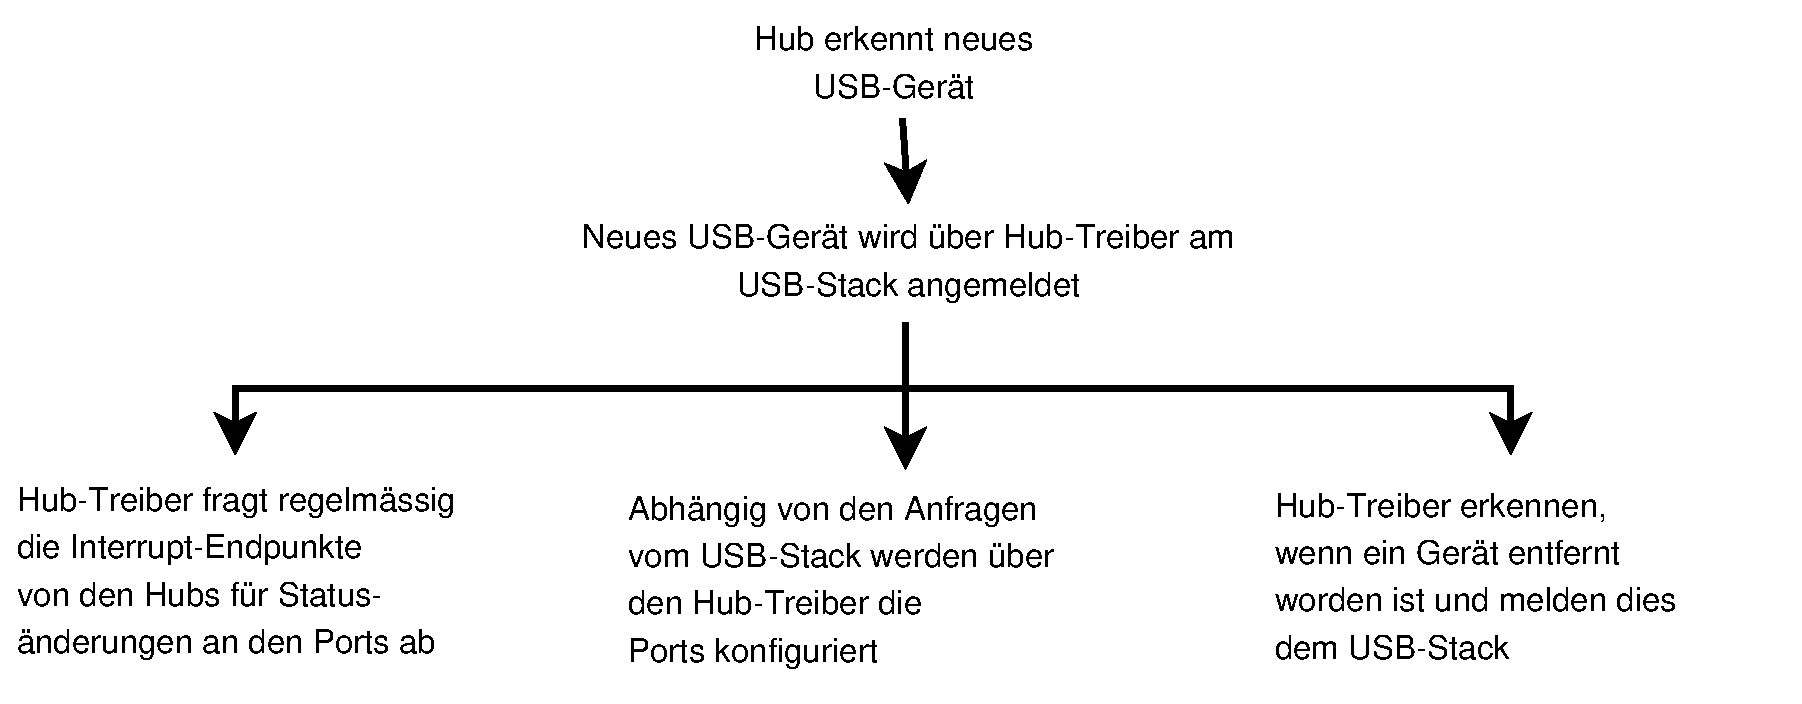
\includegraphics[width=14cm]{images/hub}
\caption{Hub-Treiber Ablauf}
\label{hub}
}
\end{figure}

\subsection{Massenspeichertreiber}
\index{Massenspeicher-Treiber}
Viele USB-Ger�te bieten ein Massenspeicher-Interface an,
da �ber dies ganz einfach standardisiert Daten ausgetauscht werden k�nnen.
F�r die Ansteuerung der Ger�te werden �ber USB SCSI-Kommandos versendet.
Das hat den gro�en Vorteil, dass leicht USB-Treiber f�r Ger�te
wie Festplatten, CD-Brenner, ZIP-Laufwerke, etc. geschrieben werden k�nnen,
da diese meist mit dem SCSI-Protokoll ansprechbar sind.
\newline\newline
Abbildung \ref{msdstruktur} (Seite \pageref{msdstruktur}) zeigt die Struktur f�r die Datenspeicherverwaltung. 
Auf der untersten Ebene befindet sich das Massenspeichermedium,
welches �ber SCSI-Kommandos angesteuert wird. Die SCSI-Kommandos
werden eingebettet in USB-Nachrichten zwischen USB-Host und -Ger�t
�bertragen. Der Massenspeichertreiber auf dem System des USB-Host
kann die USB-Nachrichten entgegennehmen und die SCSI-Kommandos
extrahieren. F�r den automatischen Aufbau
der SCSI-Kommandos bietet der Massenspeichertreiber Funktionen an.
Basierend auf den Funktionen kann ein Dateisystem aufgesetzt werden.

\begin{figure}[h]
{
\centering
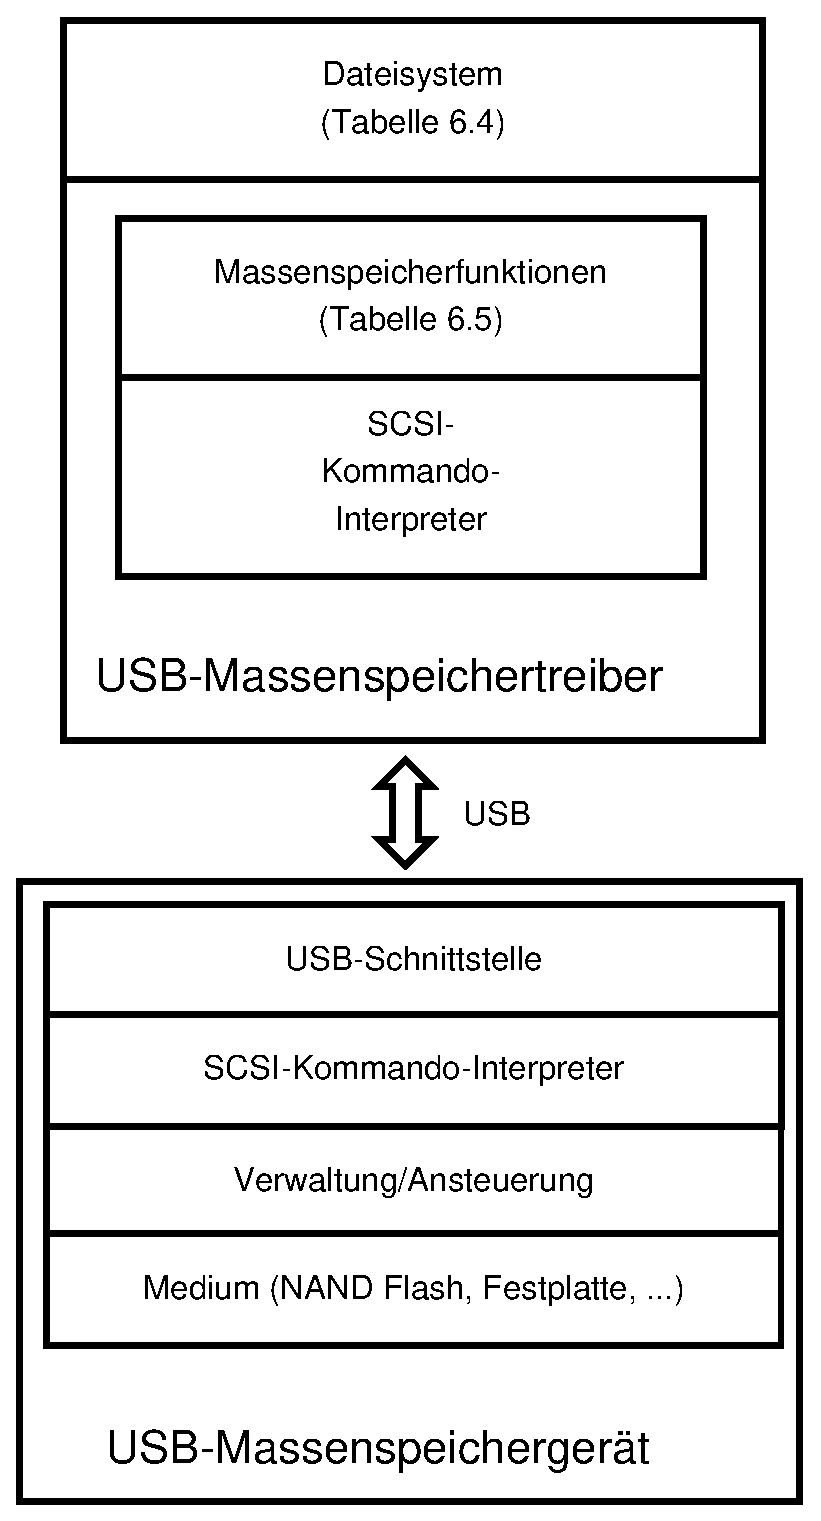
\includegraphics[height=11.5cm]{images/msdstruktur}
\caption{Struktur f�r die Datenspeicherverwaltung}
\label{msdstruktur}
}
\end{figure}

Im folgenden werden die Punkte aus der Abbildung \ref{msdstruktur} (Seite \pageref{msdstruktur})
von oben nach unten beschrieben.

\subsubsection{Embedded Dateisysteme}

Dateisysteme bieten M�glichkeiten f�r die 
Anordnung und den Zugriff auf Daten an.
Die ben�tigten Zugriffsfunktionen (siehe Tabelle \ref{usb_dateisystem_api} auf Seite \pageref{usb_dateisystem_api})
der verschiedenen Dateisysteme
unterscheiden sich, im Gegensatz zu der
Anordnung und den Strategien f�r die Verwaltung der Daten, meist wenig.
Abh�ngig vom eingesetzten Speichermedium und den Anforderungen
der Anwendungen muss das passende Dateisystem gew�hlt werden. Bei dem Entwurf
des Massenspeichertreibers muss darauf geachtet werden, dass m�glichst viele
Dateisysteme darauf aufbauen k�nnen.

\begin{table}[h]
\center
\begin{tabular}{|l|l|}
\hline
\rowcolor{Gray}[0.9\tabcolsep]
Funktion & Beschreibung \\ \hline
\text{mkdir} &  Erzeugen eines Verzeichnisses  \\ \hline
\text{chdir} &  Wechseln in ein anderes Verzeichnis \\ \hline
\text{rmdir} &  L�schen eines Verzeichnisses \\ \hline
\text{readdir} & Lesen von Verzeichniseintr�gen  \\ \hline
\text{open} & �ffnen einer Datei  \\ \hline
\text{close} & Schlie�en einer Datei  \\ \hline
\text{read} & Lesen einer Datei  \\ \hline
\text{write} & Schreiben einer Datei  \\ \hline
\text{unlink} & L�schen einer Datei  \\ \hline
\text{seek} & Positionieren des Lese- oder Schreibzeigers  \\ \hline
\end{tabular}
\caption{Ben�tigte Funktionen von Dateisystemen}
\label{usb_dateisystem_api}
\end{table}
\index{Dateisystem}


Es gibt eine Vielfalt an verschiedenen Dateisystemen f�r Embedded Systeme.
Die folgende Liste zeigt nur einen kleinen Auszug.

\begin{itemize}
\item \textbf{TINY File System} von Lucent Technologies (http://www.bell-labs.com/topic/swdist)
\item \textbf{Solid File System} von ELDOS (http://www.eldos.com/solfs/embedded.php)
\item \textbf{uc/Filesystem} von Embedded Office (http://www.embedded-office.de)
\item \textbf{FullFAT} von Holger Klabunde (http://www.holger-klabunde.de)
\item \textbf{FAT File System Module} von Elm Chan (http://elm-chan.org/)
\end{itemize}


\newpage
\subsubsection{Massenspeicherfunktionen}

Speichermedien wie Festplatten, USB-Sticks, CD-ROM Medien, etc.
haben gemeinsam, dass die Daten blockweise (ein Block entspricht einem Sektor) �bertragen und abgelegt werden.
F�r die Identifikation eines Speicherbereichs werden daher 
nicht Speicheradressen sondern Sektornummern ben�tigt.
Mit den
Funktionen aus der Tabelle \ref{usb_storage_api} kann
so abstrahiert auf viele Speichermedien zugegriffen werden.

\begin{table}[h]
\center
\begin{tabular}{|l|l|}
\hline
\rowcolor{Gray}[0.9\tabcolsep]
Funktion & Beschreibung \\ \hline
\text{void usb\_storage\_init()} &  Treiber anmelden \\ \hline
\text{u8 usb\_storage\_open(u8 device);} &  Verbindung �ffnen \\ \hline
\text{u8 usb\_storage\_read\_capacity(u8 device)} & Kapazit�t ermitteln \\ \hline
\text{u8 usb\_storage\_inquiry(u8 device)} &  Status abfragen \\ \hline
\text{void usb\_storage\_read\_sector(u8 device, u32 sector, char * buf)} &  Daten lesen \\ \hline
\text{void usb\_storage\_write\_sector(u8 device, u32 sector, char * buf)} &  Daten schreiben \\ \hline
\end{tabular}
\caption{Treiberfunktionen der Massenspeicher-Ger�teklasse, storage.h}
\label{usb_storage_api}
\end{table}
\index{storage.h}

\subsubsection{SCSI-Kommandointerpreter}

Wie bereits erw�hnt, werden USB-Massenspeicherger�te immer �ber
SCSI-Nachrichten, die �ber USB �bertragen werden, angesteuert.
Eine SCSI-Nachricht f�r ein USB-Massenspeicherger�t besteht aus zwei Paketen.
Das \glqq{}Command Block Wrapper CBW\grqq{}, das
die Anfrage enth�lt und das \glqq{}Command Status Wrapper CSW\grqq{},
das die Antwort bzw. den Status auf die Anfrage beinhaltet.
Die Datenstrukturen sind in den Listings \ref{lst:usb_cbw} und \ref{lst:usb_csw} abgedruckt.

\lstset{language=C}
\begin{lstlisting}[caption={Command Block Wrapper, storage.h},label={lst:usb_cbw},
captionpos=b,
basicstyle=\ttfamily\fontsize{10}{12}\selectfont,
commentstyle=\fontsize{10}{12}\selectfont]

typedef struct usb_storage_cbw_t usb_storage_cbw;
struct usb_storage_cbw_t {
  u32 dCBWSignature;  /* Signatur = 0x43425355 */
  u32 dCBWTag;
  u32 dCBWDataTransferLength;
  u8  bCWDFlags;      /* Enth�lt Bit f�r die Richtung */
  u8  bCBWLun;
  u8  bCBWCBLength;   /* 1 - 16 */
  u8  CBWCB[16];      /* SCSI Kommando */
};
\end{lstlisting}

\lstset{language=C}
\begin{lstlisting}[caption={Command Status Wrapper, storage.h},label={lst:usb_csw},
captionpos=b,
basicstyle=\ttfamily\fontsize{10}{12}\selectfont,
commentstyle=\fontsize{10}{12}\selectfont]

typedef struct usb_storage_csw_t usb_storage_csw;
struct usb_storage_csw_t {
  u32 dCSWSignature;	/* Signatur = 0x53425355 */
  u32 dCSWTag;		/* identisch mit dCBWTag aus Anfrage */
  u32 dCSWDataResidue;	/* identisch mit bCBWCBLength */
  u8  bCSWStatus;	/* Status �ber Erfolg */
};
\end{lstlisting}

Eingebettet in \glqq{}Command Block Wrapper CBW\grqq{} (Listing \ref{lst:usb_cbw})
werden die SCSI-Kommandos �bertragen. In der Tabelle \ref{usb_scsi} sind
die wichtigsten Kommandos aufgelistet. Der genaue Aufbau kann dem Dokument \cite{class_msd} entnommen werden.

\begin{table}[h]
\center
\begin{tabular}{|c|l|}
\hline
\rowcolor{Gray}[0.9\tabcolsep]
Kommando & Beschreibung \\ \hline
\text{0x00} & Test Unit Ready \\ \hline
\text{0x03} & Request Sense \\ \hline
\text{0x12} & Inquiry \\ \hline
\text{0x1A} & Mode Sense \\ \hline
\text{0x1E} & Prevent Allow Media Removal \\ \hline
\text{0x25} & Read Capacity \\ \hline
\text{0x28} & Read \\ \hline
\text{0x2A} & Write \\ \hline
\text{0x2F} & Verify \\ \hline
\end{tabular}
\caption{Typische SCSI-Kommandos, storage.h}
\label{usb_scsi}
\end{table}

Abbildung \ref{datenfluss_cbw} zeigt den Fluss f�r Befehle, eingehende und ausgehende Daten und den Status-Transport.

\begin{figure}[h]
{
\centering
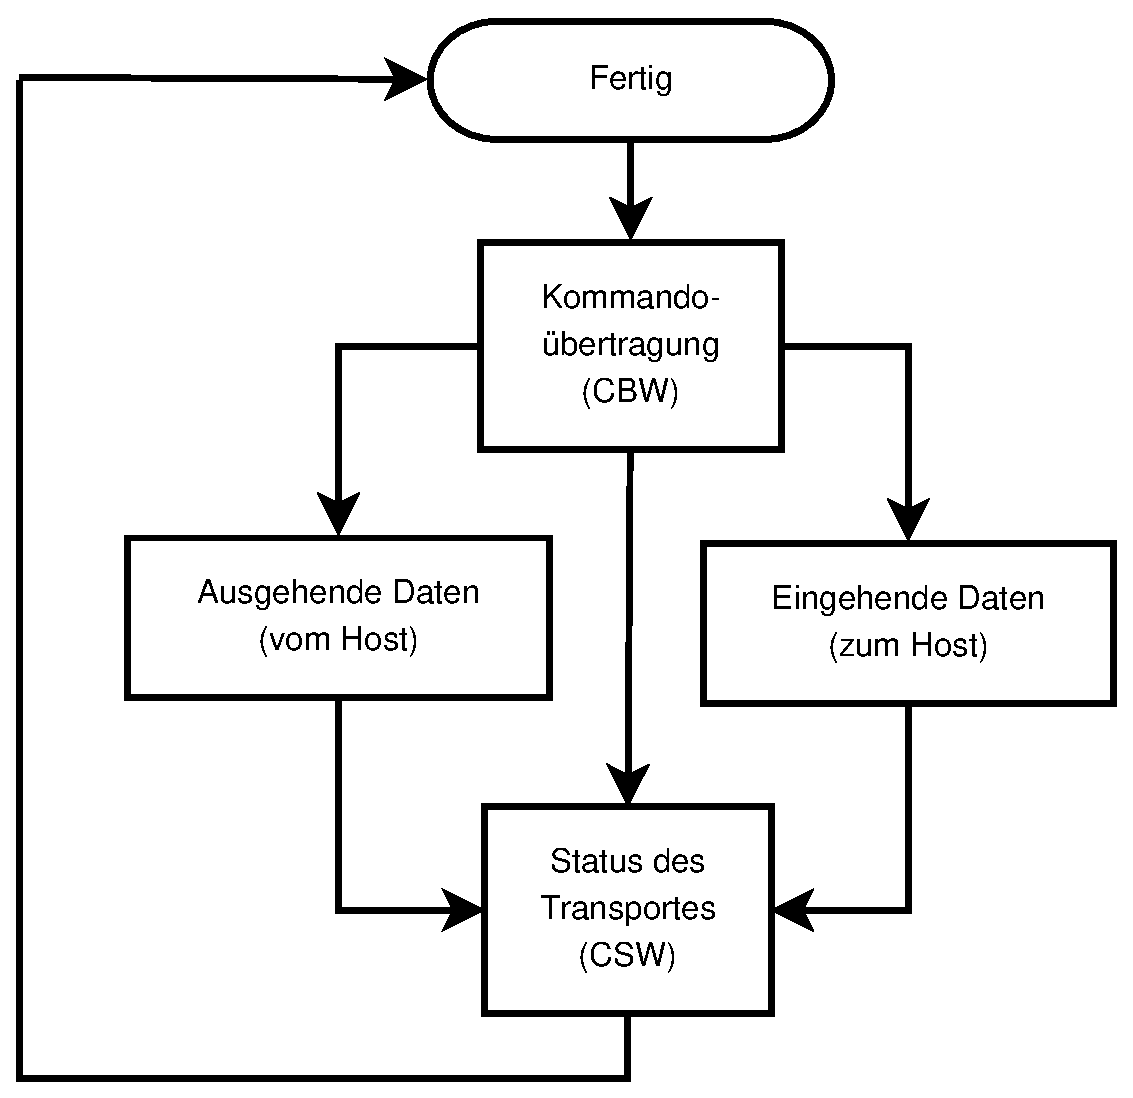
\includegraphics[height=8cm]{images/cbw_csw}
\caption{Datenfluss von CBW und CSW}
\label{datenfluss_cbw}
}
\end{figure}

Der Quelltext im Listing \ref{lst:usb_capacity} zeigt
die Implementierung der Funktion f�r das Abfragen der Speicherkapazit�t eines
Massenspeicherger�ts. Im Wesentlichen wird in Zeile 12 die Klassenanfrage \textit{Bulk-Only Mass Storage Reset}
an das Ger�t gesendet (mehr zu dieser Anfrage in Abschnitt \ref{bulk_reset} auf Seite \pageref{bulk_reset}).
Desweiteren wird der Command Block Wrapper mit dem SCSI-Kommando f�r die Abfrage der Kapazit�t 
aufgebaut und anschlie�end an das Ger�t gesendet. Als Antwort erh�lt man die Sektorgr�sse
und die Anzahl der Sektoren, woraus man sich wiederum die Kapazit�t durch Multiplikation
der beiden Faktoren ermitteln kann.

\lstset{language=C}
\begin{lstlisting}[caption={Abfrage der Speicherkapazit�t eines Massenpeicherger�ts, storage.c},label={lst:usb_capacity},
captionpos=b,
numbers=left,
basicstyle=\ttfamily\fontsize{10}{12}\selectfont,
commentstyle=\fontsize{10}{12}\selectfont]
u8 usb_storage_read_capacity(u8 device, char * size)
{
  /* send cwb "usbc" */
  char tmp[8];
  u8 i;
  u32 size;
  usb_storage_cbw  * cbw = (usb_storage_cbw*)malloc(sizeof(usb_storage_cbw));

  usb_control_msg(massstorage[device], 0x02,1,0, 0x8100, 0,tmp, 8, 0); 

  cbw->dCBWSignature= 0x43425355;
  cbw->dCWBTag=0x826A6008;
  cbw->dCBWDataTransferLength=0x00000008;
  cbw->bCWDFlags=0x80;
  cbw->bCBWLun=0x00;
  cbw->bCBWCBLength=0x0A;

  for(i=0;i<16;i++)
    cbw->CBWCB[i]=0x00;

  cbw->CBWCB[0]=0x25; // SCSI: Speicherkapazit�t abfragen

  usb_bulk_write(massstorage[device], 2, (char*)cbw, 31, 0);
  usb_bulk_read(massstorage[device], 1, (char*)cbw, 8, 0);
  
  /* Ersten 4 Byte = Max. Sector Adresse, zweiten 4 Byte = Sectorgr�sse */
  for(i=0;i<8;i++)
    size[i]=cbw[i];

  usb_bulk_read(massstorage[device], 1, (char*)cbw, 13, 0);

  free(cbw);

  return 0;
}
\end{lstlisting}





\subsubsection{USB-Schnittstelle}
Die USB-Klassenspezifikation f�r Massenspeicher bietet verschiedene Endpunkt-Konfigurationen
f�r den Betrieb an. Die einfachste und am meisten implementierte Konfiguration
ist die sogenannte \glqq{}Bulk-Only\grqq{} Methode. Hierbei werden die Daten
�ber einen eingehenden und ausgehenden Bulk-Endpunkt �bertragen.
Das Betriebssystem oder die Anwendung kann �ber den Klassencode 0x08 
und den Interface-Protokoll-Code 0x50 erkennen, dass es sich um ein Bulk-Only-Ger�t handelt.
\newline\newline
Au�erdem muss jedes Bulk-Only-Ger�t die folgenden beiden Klassen-Anfragen
beantworten k�nnen.
\label{bulk_reset}
\newline\newline
\textbf{Bulk-Only Mass Storage Reset}\newline\newline
Diese Anfrage wird ben�tigt, um das Massenspeicherger�t zu reseten. Nachfolgend
der Anfrage muss das Massenspeicherger�t auf ein Command-Block-Wrapper-Paket 
sofort antworten k�nnen. Um den Reset auszul�sen, muss die Anfrage wie folgt aufgebaut sein:
\begin{itemize}
\item \textit{bmRequestType:} Klasse, Interface, Host zu Ger�t
\item \textit{bRequest} 255 (0xFF)
\item \textit{wValue} 0
\item \textit{wIndex} Interface-Nummer
\item \textit{wLength} 0
\end{itemize}


\textbf{Get Max LUN}\newline\newline
In einem Massenspeicherger�t k�nnen mehrere logische Speicherbereiche
genutzt werden. �ber die sogenannte \glqq{}Logical-Unit-Number\grqq{}
kann ein Bereich ausgew�hlt werden. Mit der Klassen-Anfrage kann ermittelt
werden, wieviele dieser logischen Bereiche existieren.

\begin{itemize}
\item \textit{bmRequestType:} Klasse, Interface, Ger�t zu Host
\item \textit{bRequest} 254 (0xFE)
\item \textit{wValue} 0
\item \textit{wIndex} Interface-Nummer
\item \textit{wLength} 1 
\end{itemize}


\subsubsection{SCSI-Kommandointerpreter, Verwaltung/Ansteuerung, Medium}
Die letzten drei Ebenen werden unabh�ngig vom Treiber im USB-Ger�t
realisiert und sind daher f�r den Entwurf des Massenspeichertreibers
nicht von Bedeutung.






	
\chapter{Testplatine und Entwicklungsumgebung}
\index{Testplatine}
\index{Entwicklungsumgebung}
Im Rahmen der Diplomarbeit wurde eine Test- und Entwicklungsplatine f�r
die Entwicklung des USB-Stacks entworfen.

\section{Anforderungen an die Schaltung}

Prim�r dient die Schaltung dazu, die Funktionen des USB-Stacks mit USB-Ger�ten
�berpr�fen zu k�nnen. Da die Platine selbst ge�tzt und best�ckt werden sollte, wurde auf
den Einsatz von SMD-Bauteilen verzichtet.
\newline\newline
Folgende Anforderungen wurden an die Platine gestellt:

\begin{itemize}
\item Eine RS232-Schnittstelle f�r Statusmeldungen
\item Einfache Programmierm�glichkeit f�r den eingesetzten Mikrocontroller
\item Stromversorgung �ber ein USB-Kabel
\item Eine USB-Buchse f�r den USB-Port des Host-Controllers
\item Eine Leuchtdiode an einem I/O-Port f�r optische Statusmeldungen
\item Eine Layoutvorlage f�r einseitig beschichtete Platine ohne Durchkontaktierungen
\end{itemize}

\subsubsection{Eingesetzter Mikrocontroller}
Als Mikrocontroller wurde ein ATMega32 (8 Bit) der bekannten AVR-Reihe von Atmel gew�hlt.
Dieser ist preiswert zu erwerben und hat gen�gend Ports f�r die Anbindung eines
Host-Controllers. Weiterhin gibt es f�r die AVR-Controller-Reihe viele freie Programme
f�r die Softwareentwicklung.
\newline\newline
Technische Daten:
\begin{enumerate}
\item 32 KB Programmspeicher (Flash)
\item 2 KB Arbeitsspeicher (RAM) 
\item 1 KB Datenspeicher (EEPROM) 
\item Bei 16 MHz bis zu 16 MIPS\footnote{\label{foot:usbdi}\glqq{}Millionen Instruktionen pro Sekunde\grqq{} ist ein Ma� f�r die Leistungsf�higkeit von Prozessoren.}
\item 20 nach au�en gef�hrte I/O-Leitungen
\item 5 V Betriebs- und I/O-Spannung
\end{enumerate}
\subsubsection{Eingesetzter Host-Controller}
\index{SL811HS}
Ein einfacher und bew�hrter USB-Host-Controller ist der SL811HS von Cypress.
Da der SL811HS speziell f�r Embedded Systeme entwickelt worden ist,
kann er �ber eine einfache Standard-Bus-Schnittstelle angesteuert werden.
Der Controller kann in den Betriebsarten Host und Slave verwendet werden,
jedoch  ist f�r die vorliegende Diplomarbeit nur der Hostbetrieb interessant.
Den SL811HS gibt es in den Bauformen TQFP und PLCC. Das PLCC-Geh�use ist ideal
f�r Prototypen, da es f�r diese Bauform Sockel gibt, mit denen man den Controller
einfach austauschen kann.
\newline\newline
Die wichtigsten Eigenschaften des USB-Host-Controllers:
\begin{enumerate}
\item Kompatibel zur USB Spezifikation 1.1
\item Automatische Erkennung von \glqq{}Low-\grqq{} und \glqq{}Full-\grqq{} Speed-Ger�ten
\item 8-Bit bidirektionale Port-Schnittstelle
\item Integrierter Root-Hub
\item 256 Byte interner Speicher
\item 5 V-tolerante Portleitungen
\item Viele automatische Routinen f�r den USB-Betrieb wie z.B. SOF-Generierung, CRC5-Pr�fsummenerstellung, und andere. 
\end{enumerate}
\label{kap:sl811}

Das Blockdiagramm in Abbildung \ref{sl811hs} zeigt die interne Struktur im Host-Controller
Baustein SL811HS. Auf der linken Seite befindet sich der Root-Hub,
welcher die Schnittstelle zum USB-Kabel zu den Ger�ten ist. Direkt
nach dem Root-Hub befindet die SIE (\glqq{}Serial Interface Engine\grqq{})
welche die Daten entsprechend wie in Kapitel \ref{kap:signal} (Seite \pageref{kap:signal}) verarbeitet.
Die SIE ben�tigt f�r die Abtastung und die �bertragung der Daten einen konstanten Takt von 48 MHz, welcher
�ber den Taktgenerator zugef�hrt wird. Ebenfalls ben�tigt die SIE noch
die Information, ob der Baustein als Master oder Slave betrieben wird. Abh�ngig
von der gew�hlten Betriebsart werden desweiteren verschiedene Interrupts vom Interrupt-Controller
ausgel�st, weshalb eine Verbindung zwischen dem Master/Slave-Controller und dem Interrupt-Controller besteht. 
Die Prozessorschnittstelle auf der rechten Seite erm�glicht den Zugriff
auf die internen Register und den internen Speicher des SL811HS-Host-Controllers.

\begin{figure}[h]
{
\centering
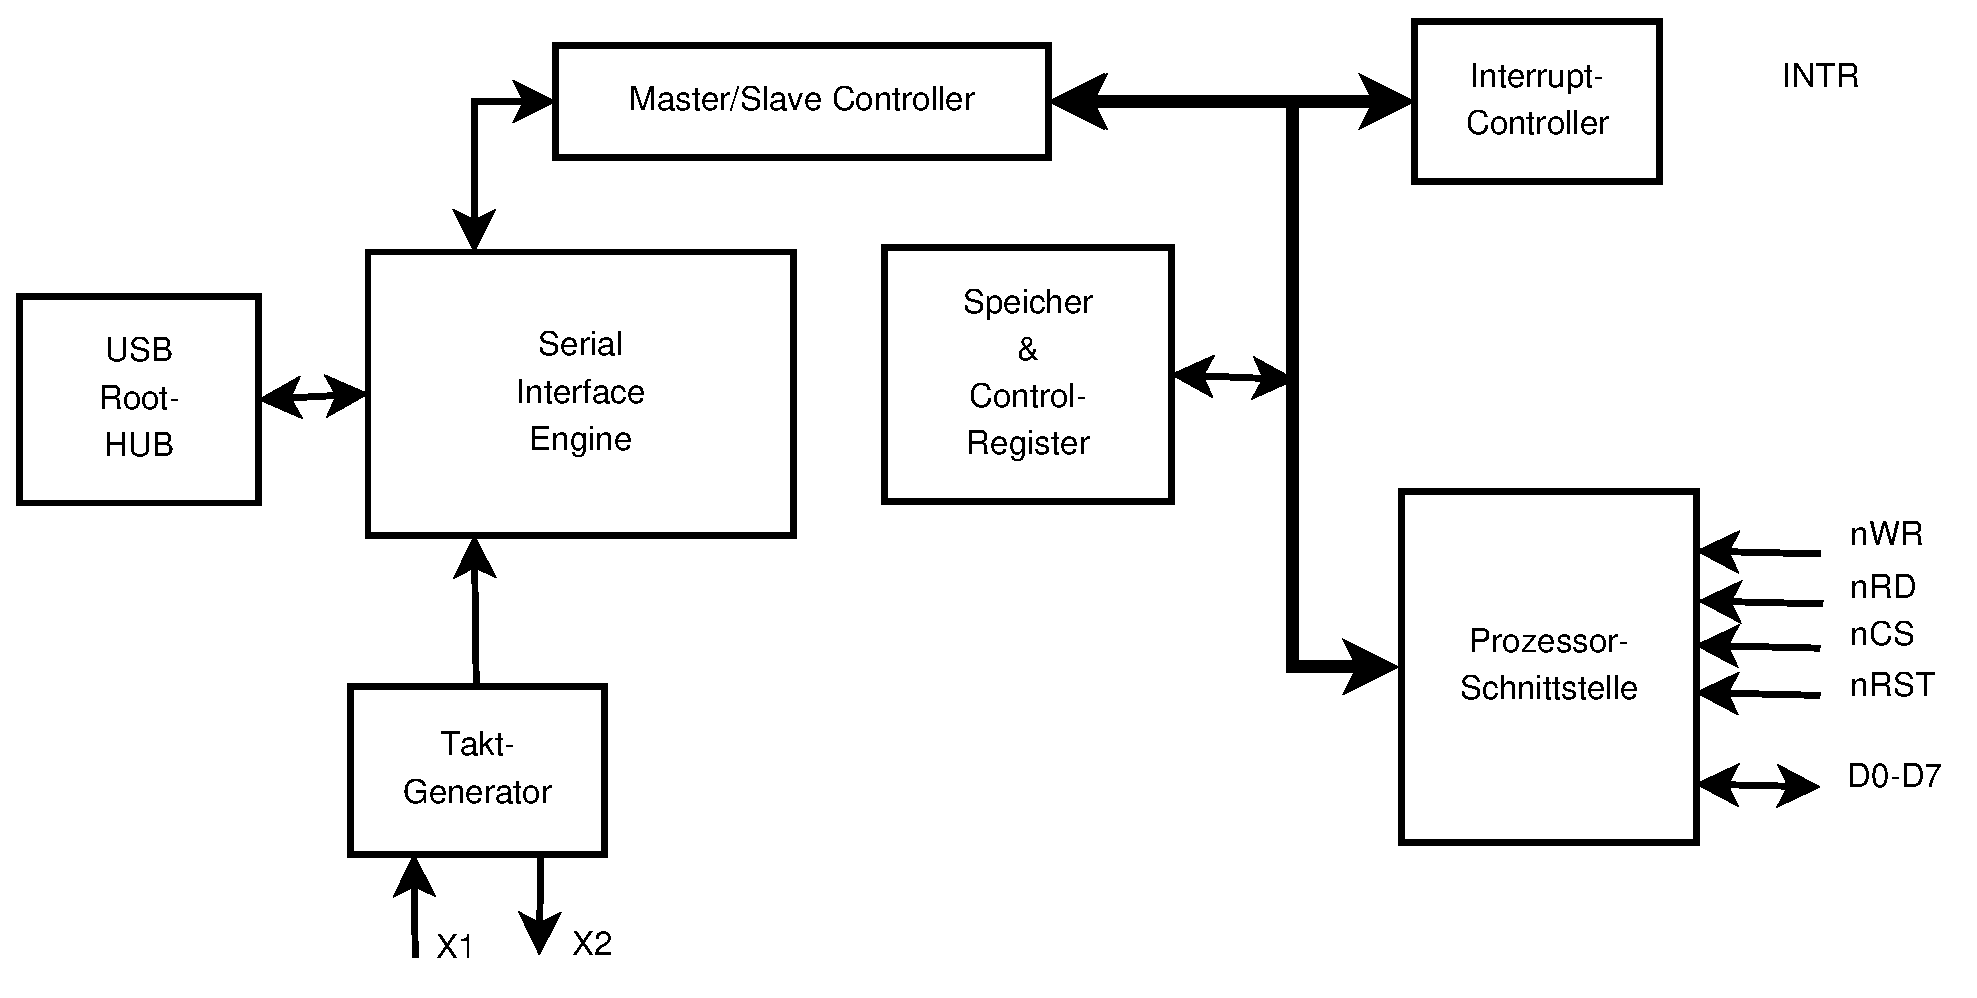
\includegraphics[width=14cm]{images/sl811hs_block}
\caption{Blockdiagramm SL811HS}
\label{sl811hs}
}
\end{figure}

\subsubsection{Entwurf der Schaltung}
Die Schaltung (siehe Abbildung \ref{schaltplan} auf Seite \pageref{schaltplan}) enth�lt nur die absolut notwendigen Bauteile. F�r die Stromversorgung
wurde die USB-Buchse X1 montiert. Dadurch kann die Testplatine �ber
ein einfaches USB-Kabel mit Strom von einem Computer versorgt werden.
Auf der Platine befinden sich der Host-Controller SL811HS,
ein RS232-Pegelwandler f�r Debugausgaben und der Mikrocontroller ATMega32 als Controller,
der die USB-Stack-Firmware ausf�hrt.
Da der SL811HS mit 3,3V versorgt werden muss, ist auf der Unterseite der Platine
ein Spannungsregler angebracht. Als Taktquelle ben�tigt
der Host-Controller entweder eine 12 MHz oder 48 MHz Taktquelle.
In der Schaltung wurde ein
externer 48 MHz Quarzoszillator eingebaut. Da der SL811HS sowohl
als Host-Controller als auch als USB-Ger�t eingesetzt werden kann, ist darauf
zu achten, dass die Signalleitung M/S (\glqq{}Pin Master/Slave Select\grqq{}) entsprechend richtig konfiguriert wird.
Der Mikrocontroller wird ebenfalls mit einem externen 16 MHz Quarz versorgt.
%Es besteht
%die M�glichkeit, auch einen internen Oszillator zu aktivieren.
%Da dieser aber nicht so genau ist, wurde auf einen externen zur�ckgegriffen.
\newline\newline
In Abbildung \ref{bestueckung} ist der Best�ckungsplan und das
Layout der Platine abgedruckt.
\begin{figure}[hpt]
{
\centering
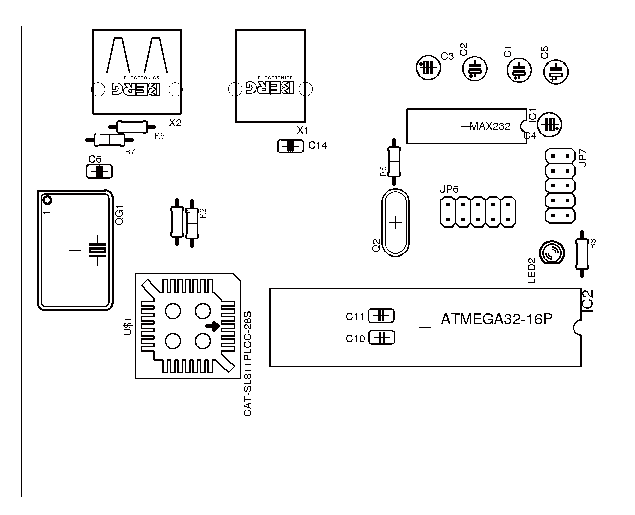
\includegraphics{images/bestueckung}
\hfill
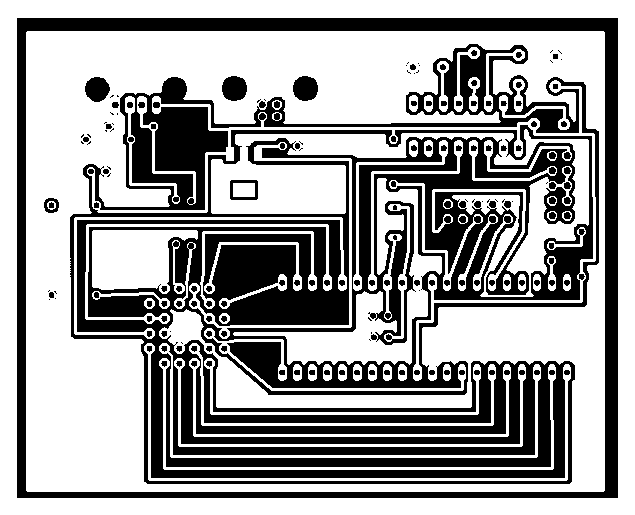
\includegraphics{images/layout}
\caption{Best�ckungsplan und Layout der Platine}
\label{bestueckung}
}
\end{figure}

%\begin{figure}[h]
%{
%\centering
%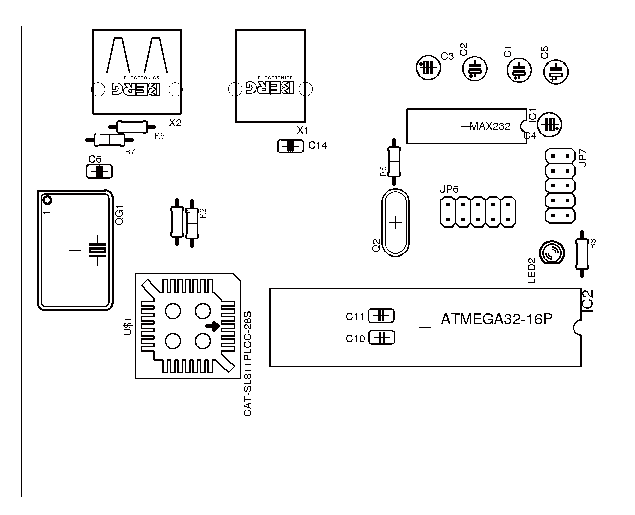
\includegraphics[height=7cm]{images/bestueckung}
%\caption{Best�ckungsplan der Testplatine}
%\label{bestueckung}
%}
%\end{figure}

%\begin{figure}[h]
%{
%\centering
%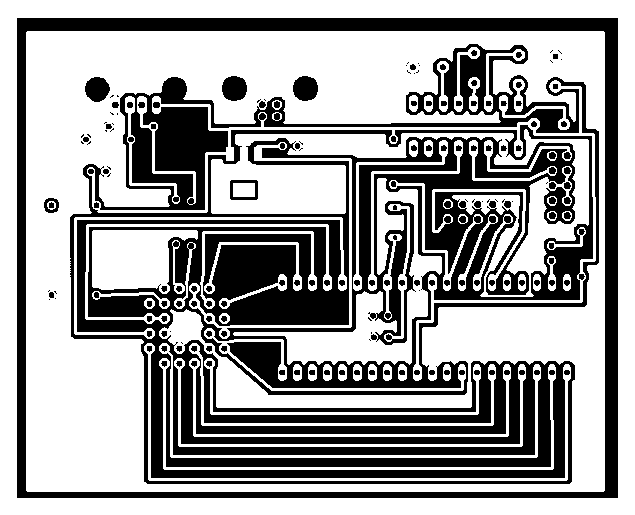
\includegraphics[height=7cm]{images/layout}
%\caption{Layout der Testplatine}
%\label{layout}
%}
%\end{figure}
%\newpage


\section{Entwicklungsumgebung}
Da die Diplomarbeit ein Open-Source-Projekt werden soll,
wurde bei der Entwicklung darauf geachtet, dass nur mit
freien oder zumindest kostenlosen Programmen gearbeitet wurde.
\newline\newline
Der Entwicklungsaufbau sah wie in Abbildung \ref{entwicklung} dargestellt aus.
Der Computer, der als Entwicklungsplattform dient, 
ist mit der Testplatine �ber ein RS232- und einem USB-Kabel f�r die Stromversorgung 
verbunden. Programmiert wird der Mikrocontroller ATMega32 �ber einen extra USB-Adapter \cite{usbprog}.
Der USB-Port ist die Schnittstelle f�r USB-Ger�te f�r die Treiberentwicklung zum Software-Stack hin.
\begin{figure}[h]
{
\centering
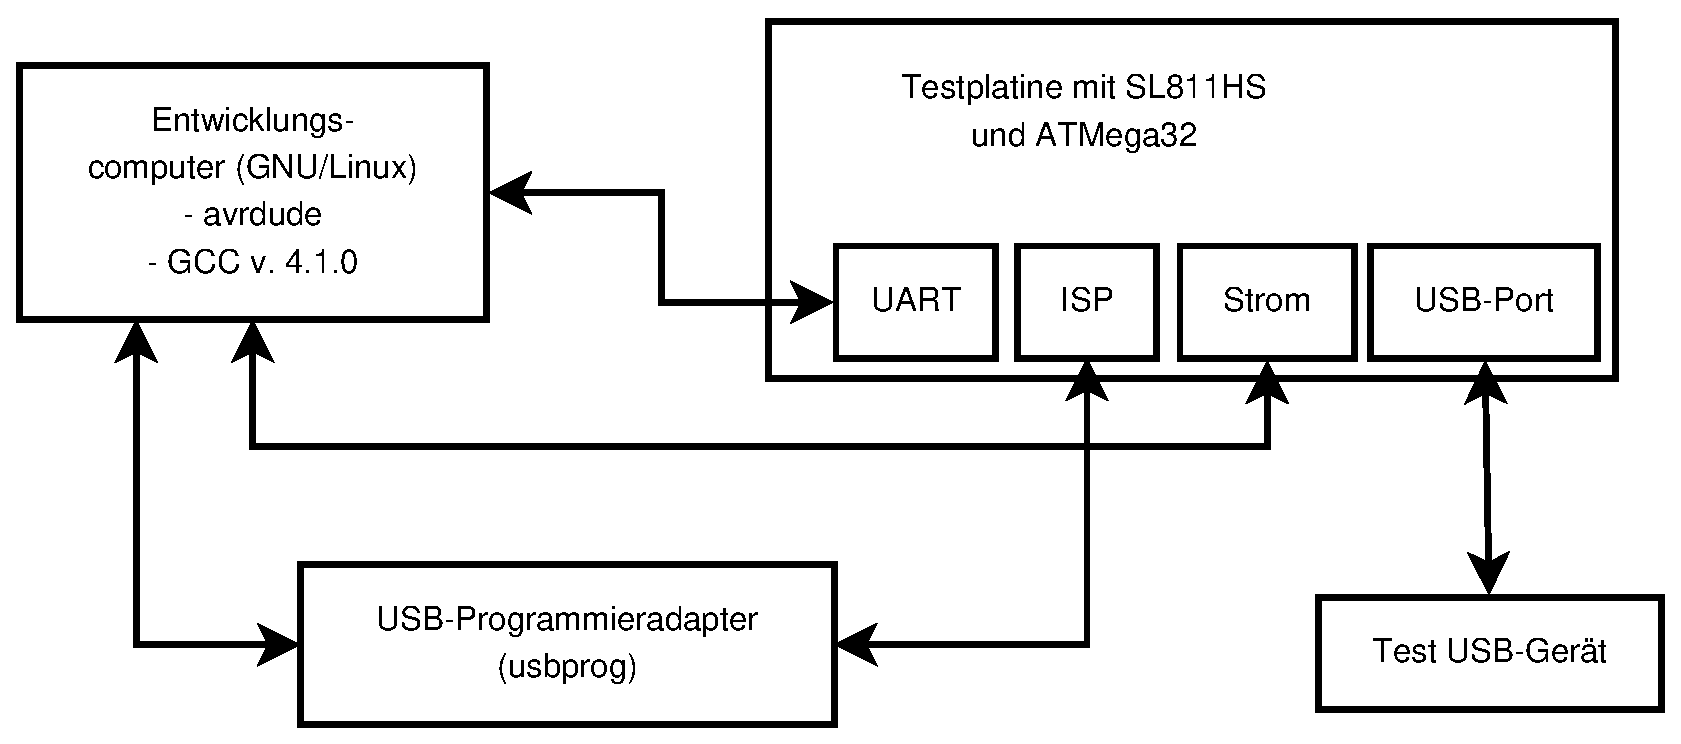
\includegraphics[width=14cm]{images/entwicklung}
\caption{Entwicklungsumgebung}
\label{entwicklung}
}
\end{figure}
\newline\newline
F�r die Hardwareentwicklung wurden folgende Programme und Ger�te verwendet:

\begin{itemize}
\item Eagle v. 3.5\cite{eagle}, Freeware, zum Zeichnen des Schaltplans und Setzen des Layouts f�r die Platine.
\item avrdude\cite{avrdude}, Open-Source, f�r die Programmierung des Mikrocontrollers.
\item usbprog\cite{usbprog}, Open-Source-Hardware, Programmieradapter f�r AVR Mikrocontroller.
\end{itemize}

F�r die Software kamen folgende Programme zum Einsatz:

\begin{itemize}
\item GCC f�r Linux Version 4.1.0\cite{gcc}, Open-Source, freier C Compiler.
\item Kermit\cite{kermit}, Open-Source, Terminal (wurde f�r die Debugausgaben �ber RS232 ben�tigt).
\end{itemize}

Die Liste der zur Verf�gung stehenden USB-Ger�te w�hrend des Entwurfs:

\begin{itemize}
\item \glqq{}Hi-Speed USB 2.0\grqq{} Hub von equip.
\item \glqq{}USB-Modul UM100 (FT232AM)\grqq{} von ELV.
\item \glqq{}MP3-Player Lyra\grqq{} von Thomson (als Massenspeicher).
\item \glqq{}1 GB USB Flash Speicher Stick\grqq{} von PNY.
\item \glqq{}AVR JTAGICE mk2\grqq{} von Atmel.
\item \glqq{}E232 Drucker\grqq{} von Lexmark.
\end{itemize}

Die Vielfalt war vor allem f�r das Testen der Enumerierung sehr wichtig.

\begin{figure}
{
\centering
\includegraphics[scale=0.7]{schaltplan.ps}
\caption{Schaltplan der Testplatine}
\label{schaltplan}
}
\end{figure}


	\chapter{Fazit und Ausblick}
\section{Fazit}
Ziel der Diplomarbeit war es, einen freien, portablen
und erweiterbaren USB-Host-Stack f�r Embedded-Systeme zu entwickeln.
Um einen einfach einsetzbaren und vollst�ndigen USB-Host-Stack
erstellen zu k�nnen, musste viel Arbeit in das Design der Softwarestruktur investiert werden.
Denn nur mit einer klaren und �bersichtlichen Struktur k�nnen andere
Entwickler daf�r begeistert werden, diesen USB-Stack zu nutzen.
Die klare Struktur wurde mit einer Aufteilung in einzelne Komponenten
und Treiber erreicht. F�r den USB-Host-Stack wurden in der Diplomarbeit
ein Host-Controller-Treiber f�r den Baustein SL811HS von Cypress, 
ein USB-Ger�tetreiber f�r den USB zu RS232 Wandler FT232 von FTDI Inc.
und USB-Klassentreiber f�r Massenspeicher, Hub- und HID-Ger�te entwickelt.
\newline\newline
Mit Hilfe von Beispielanwendungen wird dem Anwender
der Einstieg erleichtert. Desweiteren
wurde viel Wert auf die Kommentierung des Quelltextes gelegt, um
die Lesbarkeit f�r interessierte Entwickler zu erh�hen.
Die n�chsten Arbeiten an diesem Projekt werden erstrangig
die Ver�ffentlichung als Open-Source-Projekt und die Entwicklung von weiteren Host-Controller-Treibern
sein. 
\newline\newline
Der USB-Stack hat gemessen an den implementierten und noch geplanten
Features das Potenzial, eine echte Konkurrenz zu den kommerziell verf�gbaren USB-Stacks
zu werden. 



\section{Ausblick}

Im letzten Kapitel der Diplomarbeit soll
ein Ausblick auf m�gliche weitere Entwicklungen gegeben werden.
Dabei interessiert speziell die Funktionsweise des neuesten USB Standards OTG.
Dieser Standard wird nicht von der aktuellen
Version des USB-Stacks der Diplomarbeit unterst�tzt,
soll aber, nachdem das Projekt als Open-Source-Projekt freigegeben wurde,
integriert werden. Zum Abschluss der Arbeit wird ein kleiner Blick
in die Zukunft gewagt, um zu sehen, wie eine weitere Entwicklung aussehen k�nnte.

\subsubsection{USB-OTG-Standard}
\index{OTG}
\index{USB-OTG-Standard}
\index{Host-Negotiation-Protcol}
\index{Session-Request-Protocol}
Wie in den vorangegangenen Kapiteln aufgef�hrt, werden f�r
die Kommunikation stets ein fester Host-Controller 
und dedizierte USB-Ger�te ben�tigt. Sollen 
Daten zwischen zwei Ger�ten ausgetauscht werden,
muss dies immer �ber den Host-Controller geschehen.
\newline\newline
Mit dem USB-OTG-Standard (\glqq{}On-The-Go\grqq{}) wurde eine M�glichkeit geschaffen,
Daten direkt zwischen zwei Ger�ten auszutauschen.
Beispielsweise kann eine Digitalkamera Daten ohne zwischengeschalteten Computer an einen Drucker senden.
\newline\newline
Bereits wie beim �bergang von der Version USB 1.1 auf 2.0 wurde
der �bergang zum OTG-Standard ebenfalls so umgesetzt, dass alle Ger�te r�ckw�rtskompatibel
zu den vorangegangenen Versionen sind. F�r die OTG-Funktionalit�t
wurden haupts�chlich zwei neue Protokolle
eingef�hrt - das \glqq{}Host-Negotiation-Protocol\grqq{} (HNP)
und das \glqq{}Session-Request-Protocol\grqq{} (SRP).
\newline\newline
\textbf{Host-Negotiation-Protocol (HNP)}\newline\newline
Das besondere an USB-OTG
ist, dass ein Ger�t keine feste Rolle hat, sondern
diese erst beim Verbinden mit anderen Ger�ten in Abh�ngigkeit von der Anwendung 
ausgehandelt wird (entweder Host oder Slave).
\newline\newline
Dass ein Ger�t keine feste Rolle hat, ist aber nicht ganz korrekt,
denn in der OTG-Spezifikation wird immer
von einem A-Ger�t und B-Ger�t gesprochen, welche 
unterschiedliche USB-Buchsen haben.
Da USB-Kabel ebenfalls auf der einen Seite immer einen A-Stecker und auf der anderen einen B-Stecker
haben, kann man immer nur ein A-Ger�t mit einem B-Ger�t verbinden.
Zu Beginn jeder Kommunikation ist das A-Ger�t immer der Host und das B-Ger�t
das klassische USB-Ger�t.
\newline\newline
Der Ablauf nach dem Anstecken sieht im Groben wie folgt aus:

\begin{enumerate}
\item Das A-Ger�t arbeitet als Host und das B-Ger�t als USB-Funktion.
\item Das A-Ger�t generiert SOF, Bus Reset, etc. und enumeriert das B-Ger�t.
\item Das A-Ger�t fragt w�hrend der Enumeration den OTG-Deskriptor ab.
\item Dem OTG-Deskriptor kann entnommen werden, welche OTG-Unterst�tzungen das B-Ger�t hat.
\item Wenn das B-Ger�t Host werden soll, sendet das A-Ger�t die Standardanfrage SetFeature mit 
der gew�nschten Eigenschaft ab.
\item Das B-Ger�t hat nun die M�glichkeit, den Bus zu �bernehmen, denn das A-Ger�t stoppt und
l�st die Verbindung zum Bus f�r mindestens 3 ms.
\end{enumerate}

Der genaue Ablauf kann der USB-On-the-go-Spezifikation entnommen werden \cite{onthego}.
\newline\newline
\textbf{Session-Request-Protocol (SRP)}\newline\newline
Durch das \glqq{}Session Request Protocol\grqq{} k�nnen die Ger�te
aushandeln, welches Ger�t den USB-Bus mit Strom versorgt. Hierf�r
werden Mechanismen ben�tigt, so dass jedes Ger�t in den Standby-Modus 
umschalten und wieder vom Kommunikationspartner aufgeweckt werden
kann. 
Das Protokoll wird �ber verschiedene elektrische Signale
auf den Leitungen umgesetzt, z.B. dienen regelm��ige Signale (Impulse)
oder verschiedene Spannungsgrenzen als Signalisierung f�r bestimmte Zust�nde.

\subsubsection{Zuk�nftige Entwicklungen}

Die Entwicklung des USB-Stacks soll nach der Abgabe der Diplomarbeit als
Open Source Projekt weitergehen. Die Ideenliste f�r weitere Entwicklungen
ist noch lang.
\begin{itemize}
\item Weitere Host-Controller-Treiber entwickeln (AT90USB, ISP1161, etc.)
\item Mehr Ger�tetreiber anbieten (WLAN-Sticks, Bluetooth, GPS, etc.)
\item Neue Klassentreiber schreiben (Netzwerkkarten, Drucker, etc.)
\item Einen USB-Device-Stack integrieren
\item Den neuen Standard OTG implementieren
\item F�r h�here �bertragungsraten USB 2.0 High-Speed-Support hinzuf�gen
\item Einen freien USB-Sniffer entwerfen
%Da die Enwicklung von Host-Controller-Treibern ohne sogenannte \glqq{}USB-Sniffer\grqq{}\footnote{\label{foot:1 ein Ger�t, das zwischen
%eine USB-Verbdinung eingeh�ngt werden kann um die Pakete auf dem USB Bus mit aufzuzeichnen
%sehr m�hs�lig ist, wurden bereits mit ersten Tests begonnne, wie man so einen
%Sniffer ganz einfach aufbauen k�nnte, und so nicht einige Hundert Euro ausgeben muss.
\item einen IP-Host-Controller in VHDL oder Verilog inkl. passendem Treiber hinzuf�gen
\item USB-Stack als Kommunikationsstack in ein Echtzeitbetriebssystem f�r eingebettete Systeme integrieren
\end{itemize}








	%\include{kapitel9}
    % Anhang
    \begin{appendix}
      % hier kommen die Abschnitte des Anhangs hin
      \chapter{Abk�rzungsverzeichnis}
%
\renewcommand{\arraystretch}{1.5}
%
\begin{longtable}{ll}
%
ANSI & American National Standards Institute\\
API & Application Programming Interface\\
CDC & Communication Device Class\\
DPLL & Digital Phase Locked Loop \\
EHCI & Enhanced Host Controller Interface\\
GND & Ground\\
HCD & Host Controller Driver\\
HCDI & Host Controller Driver Interface\\
HNP & Host Negotiation Protocol\\
IP & Intellectual Property\\
IRP & I/O Request Paket\\
NRZI & Non Return to Zero\\
OHCI & Open Host Controller Interface\\
OTG & On the Go\\
PC & Personal Computer\\
SCSI & Small Computer System Interface\\
SIE & Serial Interface Engine\\
SRP & Session Request Protocol\\
TD & Transfer Deskriptor\\
USB & Universal Serial Bus\\
USBD & Universal Serial Bus Driver\\
USBDI & Universal Serial Bus Driver Interface\\
UHCI & Universal Host-Controller Interface\\
VCC & Voltage of the common collector \\
\end{longtable}
%
%\renewcommand{\arraystretch}{1}

      %\begingroup
\renewcommand*{\chapterheadendvskip}{\vskip 0cm}
%\cleardoublepage
\chapter{Schaltplan}
\enlargethispage{100cm}
%\cleardoublepage
\includegraphics[scale=0.7]{schaltplan.ps}
\endgroup


      \chapter{Quelltexte}
Der gedruckten Ausgabe der Diplomarbeit ist eine CD-ROM mit dem Quelltext
des USB-Host-Stacks beigelegt. Auf der CD befinden sich ebenfalls das originale
\TeX{} Dokument und eine PDF-Ausgabe der Diplomarbeit.
\newline\newline
Die neueste Version des Quelltextes kann von folgendem SVN-Archiv heruntergeladen werden:
\newline\newline
\textit{svn checkout svn://svn.berlios.de/usbport/trunk}

\begin{verbatim}
Verzeichnisstruktur auf der CDROM:

arch          Beispielimplementierungen f�r verschiedene Mikrocontroller
boards        Schaltplan, Platinenlayout, etc. f�r die Testplatine
core          USB-Kern-Funktionen
doc           Diplomarbeit als Beschreibung
drivers       USB-Treiber (Ger�te und Klassen)
host          Host-Controller-Treiber
lib           Zusatzfunktionen, Typendefinitionen, etc.
uclibusb      USB-Bibliotheken f�r USB-Ger�te
usbspec       Datentypen und -formate der USB-Spezifikation
\end{verbatim}

      \chapter{GNU Free Documentation License}
\begin{verbatim}
              GNU Free Documentation License
                Version 1.2, November 2002


 Copyright (C) 2000,2001,2002  Free Software Foundation, Inc.
     51 Franklin St, Fifth Floor, Boston, MA  02110-1301  USA
 Everyone is permitted to copy and distribute verbatim copies
 of this license document, but changing it is not allowed.


0. PREAMBLE

The purpose of this License is to make a manual, textbook, or other
functional and useful document "free" in the sense of freedom: to
assure everyone the effective freedom to copy and redistribute it,
with or without modifying it, either commercially or noncommercially.
Secondarily, this License preserves for the author and publisher a way
to get credit for their work, while not being considered responsible
for modifications made by others.

This License is a kind of "copyleft", which means that derivative
works of the document must themselves be free in the same sense.  It
complements the GNU General Public License, which is a copyleft
license designed for free software.

We have designed this License in order to use it for manuals for free
software, because free software needs free documentation: a free
program should come with manuals providing the same freedoms that the
software does.  But this License is not limited to software manuals;
it can be used for any textual work, regardless of subject matter or
whether it is published as a printed book.  We recommend this License
principally for works whose purpose is instruction or reference.


1. APPLICABILITY AND DEFINITIONS

This License applies to any manual or other work, in any medium, that
contains a notice placed by the copyright holder saying it can be
distributed under the terms of this License.  Such a notice grants a
world-wide, royalty-free license, unlimited in duration, to use that
work under the conditions stated herein.  The "Document", below,
refers to any such manual or work.  Any member of the public is a
licensee, and is addressed as "you".  You accept the license if you
copy, modify or distribute the work in a way requiring permission
under copyright law.

A "Modified Version" of the Document means any work containing the
Document or a portion of it, either copied verbatim, or with
modifications and/or translated into another language.

A "Secondary Section" is a named appendix or a front-matter section of
the Document that deals exclusively with the relationship of the
publishers or authors of the Document to the Document's overall subject
(or to related matters) and contains nothing that could fall directly
within that overall subject.  (Thus, if the Document is in part a
textbook of mathematics, a Secondary Section may not explain any
mathematics.)  The relationship could be a matter of historical
connection with the subject or with related matters, or of legal,
commercial, philosophical, ethical or political position regarding
them.

The "Invariant Sections" are certain Secondary Sections whose titles
are designated, as being those of Invariant Sections, in the notice
that says that the Document is released under this License.  If a
section does not fit the above definition of Secondary then it is not
allowed to be designated as Invariant.  The Document may contain zero
Invariant Sections.  If the Document does not identify any Invariant
Sections then there are none.

The "Cover Texts" are certain short passages of text that are listed,
as Front-Cover Texts or Back-Cover Texts, in the notice that says that
the Document is released under this License.  A Front-Cover Text may
be at most 5 words, and a Back-Cover Text may be at most 25 words.

A "Transparent" copy of the Document means a machine-readable copy,
represented in a format whose specification is available to the
general public, that is suitable for revising the document
straightforwardly with generic text editors or (for images composed of
pixels) generic paint programs or (for drawings) some widely available
drawing editor, and that is suitable for input to text formatters or
for automatic translation to a variety of formats suitable for input
to text formatters.  A copy made in an otherwise Transparent file
format whose markup, or absence of markup, has been arranged to thwart
or discourage subsequent modification by readers is not Transparent.
An image format is not Transparent if used for any substantial amount
of text.  A copy that is not "Transparent" is called "Opaque".

Examples of suitable formats for Transparent copies include plain
ASCII without markup, Texinfo input format, LaTeX input format, SGML
or XML using a publicly available DTD, and standard-conforming simple
HTML, PostScript or PDF designed for human modification.  Examples of
transparent image formats include PNG, XCF and JPG.  Opaque formats
include proprietary formats that can be read and edited only by
proprietary word processors, SGML or XML for which the DTD and/or
processing tools are not generally available, and the
machine-generated HTML, PostScript or PDF produced by some word
processors for output purposes only.

The "Title Page" means, for a printed book, the title page itself,
plus such following pages as are needed to hold, legibly, the material
this License requires to appear in the title page.  For works in
formats which do not have any title page as such, "Title Page" means
the text near the most prominent appearance of the work's title,
preceding the beginning of the body of the text.

A section "Entitled XYZ" means a named subunit of the Document whose
title either is precisely XYZ or contains XYZ in parentheses following
text that translates XYZ in another language.  (Here XYZ stands for a
specific section name mentioned below, such as "Acknowledgements",
"Dedications", "Endorsements", or "History".)  To "Preserve the Title"
of such a section when you modify the Document means that it remains a
section "Entitled XYZ" according to this definition.

The Document may include Warranty Disclaimers next to the notice which
states that this License applies to the Document.  These Warranty
Disclaimers are considered to be included by reference in this
License, but only as regards disclaiming warranties: any other
implication that these Warranty Disclaimers may have is void and has
no effect on the meaning of this License.


2. VERBATIM COPYING

You may copy and distribute the Document in any medium, either
commercially or noncommercially, provided that this License, the
copyright notices, and the license notice saying this License applies
to the Document are reproduced in all copies, and that you add no other
conditions whatsoever to those of this License.  You may not use
technical measures to obstruct or control the reading or further
copying of the copies you make or distribute.  However, you may accept
compensation in exchange for copies.  If you distribute a large enough
number of copies you must also follow the conditions in section 3.

You may also lend copies, under the same conditions stated above, and
you may publicly display copies.


3. COPYING IN QUANTITY

If you publish printed copies (or copies in media that commonly have
printed covers) of the Document, numbering more than 100, and the
Document's license notice requires Cover Texts, you must enclose the
copies in covers that carry, clearly and legibly, all these Cover
Texts: Front-Cover Texts on the front cover, and Back-Cover Texts on
the back cover.  Both covers must also clearly and legibly identify
you as the publisher of these copies.  The front cover must present
the full title with all words of the title equally prominent and
visible.  You may add other material on the covers in addition.
Copying with changes limited to the covers, as long as they preserve
the title of the Document and satisfy these conditions, can be treated
as verbatim copying in other respects.

If the required texts for either cover are too voluminous to fit
legibly, you should put the first ones listed (as many as fit
reasonably) on the actual cover, and continue the rest onto adjacent
pages.

If you publish or distribute Opaque copies of the Document numbering
more than 100, you must either include a machine-readable Transparent
copy along with each Opaque copy, or state in or with each Opaque copy
a computer-network location from which the general network-using
public has access to download using public-standard network protocols
a complete Transparent copy of the Document, free of added material.
If you use the latter option, you must take reasonably prudent steps,
when you begin distribution of Opaque copies in quantity, to ensure
that this Transparent copy will remain thus accessible at the stated
location until at least one year after the last time you distribute an
Opaque copy (directly or through your agents or retailers) of that
edition to the public.

It is requested, but not required, that you contact the authors of the
Document well before redistributing any large number of copies, to give
them a chance to provide you with an updated version of the Document.


4. MODIFICATIONS

You may copy and distribute a Modified Version of the Document under
the conditions of sections 2 and 3 above, provided that you release
the Modified Version under precisely this License, with the Modified
Version filling the role of the Document, thus licensing distribution
and modification of the Modified Version to whoever possesses a copy
of it.  In addition, you must do these things in the Modified Version:

A. Use in the Title Page (and on the covers, if any) a title distinct
   from that of the Document, and from those of previous versions
   (which should, if there were any, be listed in the History section
   of the Document).  You may use the same title as a previous version
   if the original publisher of that version gives permission.
B. List on the Title Page, as authors, one or more persons or entities
   responsible for authorship of the modifications in the Modified
   Version, together with at least five of the principal authors of the
   Document (all of its principal authors, if it has fewer than five),
   unless they release you from this requirement.
C. State on the Title page the name of the publisher of the
   Modified Version, as the publisher.
D. Preserve all the copyright notices of the Document.
E. Add an appropriate copyright notice for your modifications
   adjacent to the other copyright notices.
F. Include, immediately after the copyright notices, a license notice
   giving the public permission to use the Modified Version under the
   terms of this License, in the form shown in the Addendum below.
G. Preserve in that license notice the full lists of Invariant Sections
   and required Cover Texts given in the Document's license notice.
H. Include an unaltered copy of this License.
I. Preserve the section Entitled "History", Preserve its Title, and add
   to it an item stating at least the title, year, new authors, and
   publisher of the Modified Version as given on the Title Page.  If
   there is no section Entitled "History" in the Document, create one
   stating the title, year, authors, and publisher of the Document as
   given on its Title Page, then add an item describing the Modified
   Version as stated in the previous sentence.
J. Preserve the network location, if any, given in the Document for
   public access to a Transparent copy of the Document, and likewise
   the network locations given in the Document for previous versions
   it was based on.  These may be placed in the "History" section.
   You may omit a network location for a work that was published at
   least four years before the Document itself, or if the original
   publisher of the version it refers to gives permission.
K. For any section Entitled "Acknowledgements" or "Dedications",
   Preserve the Title of the section, and preserve in the section all
   the substance and tone of each of the contributor acknowledgements
   and/or dedications given therein.
L. Preserve all the Invariant Sections of the Document,
   unaltered in their text and in their titles.  Section numbers
   or the equivalent are not considered part of the section titles.
M. Delete any section Entitled "Endorsements".  Such a section
   may not be included in the Modified Version.
N. Do not retitle any existing section to be Entitled "Endorsements"
   or to conflict in title with any Invariant Section.
O. Preserve any Warranty Disclaimers.

If the Modified Version includes new front-matter sections or
appendices that qualify as Secondary Sections and contain no material
copied from the Document, you may at your option designate some or all
of these sections as invariant.  To do this, add their titles to the
list of Invariant Sections in the Modified Version's license notice.
These titles must be distinct from any other section titles.

You may add a section Entitled "Endorsements", provided it contains
nothing but endorsements of your Modified Version by various
parties--for example, statements of peer review or that the text has
been approved by an organization as the authoritative definition of a
standard.

You may add a passage of up to five words as a Front-Cover Text, and a
passage of up to 25 words as a Back-Cover Text, to the end of the list
of Cover Texts in the Modified Version.  Only one passage of
Front-Cover Text and one of Back-Cover Text may be added by (or
through arrangements made by) any one entity.  If the Document already
includes a cover text for the same cover, previously added by you or
by arrangement made by the same entity you are acting on behalf of,
you may not add another; but you may replace the old one, on explicit
permission from the previous publisher that added the old one.

The author(s) and publisher(s) of the Document do not by this License
give permission to use their names for publicity for or to assert or
imply endorsement of any Modified Version.


5. COMBINING DOCUMENTS

You may combine the Document with other documents released under this
License, under the terms defined in section 4 above for modified
versions, provided that you include in the combination all of the
Invariant Sections of all of the original documents, unmodified, and
list them all as Invariant Sections of your combined work in its
license notice, and that you preserve all their Warranty Disclaimers.

The combined work need only contain one copy of this License, and
multiple identical Invariant Sections may be replaced with a single
copy.  If there are multiple Invariant Sections with the same name but
different contents, make the title of each such section unique by
adding at the end of it, in parentheses, the name of the original
author or publisher of that section if known, or else a unique number.
Make the same adjustment to the section titles in the list of
Invariant Sections in the license notice of the combined work.

In the combination, you must combine any sections Entitled "History"
in the various original documents, forming one section Entitled
"History"; likewise combine any sections Entitled "Acknowledgements",
and any sections Entitled "Dedications".  You must delete all sections
Entitled "Endorsements".


6. COLLECTIONS OF DOCUMENTS

You may make a collection consisting of the Document and other documents
released under this License, and replace the individual copies of this
License in the various documents with a single copy that is included in
the collection, provided that you follow the rules of this License for
verbatim copying of each of the documents in all other respects.

You may extract a single document from such a collection, and distribute
it individually under this License, provided you insert a copy of this
License into the extracted document, and follow this License in all
other respects regarding verbatim copying of that document.


7. AGGREGATION WITH INDEPENDENT WORKS

A compilation of the Document or its derivatives with other separate
and independent documents or works, in or on a volume of a storage or
distribution medium, is called an "aggregate" if the copyright
resulting from the compilation is not used to limit the legal rights
of the compilation's users beyond what the individual works permit.
When the Document is included in an aggregate, this License does not
apply to the other works in the aggregate which are not themselves
derivative works of the Document.

If the Cover Text requirement of section 3 is applicable to these
copies of the Document, then if the Document is less than one half of
the entire aggregate, the Document's Cover Texts may be placed on
covers that bracket the Document within the aggregate, or the
electronic equivalent of covers if the Document is in electronic form.
Otherwise they must appear on printed covers that bracket the whole
aggregate.


8. TRANSLATION

Translation is considered a kind of modification, so you may
distribute translations of the Document under the terms of section 4.
Replacing Invariant Sections with translations requires special
permission from their copyright holders, but you may include
translations of some or all Invariant Sections in addition to the
original versions of these Invariant Sections.  You may include a
translation of this License, and all the license notices in the
Document, and any Warranty Disclaimers, provided that you also include
the original English version of this License and the original versions
of those notices and disclaimers.  In case of a disagreement between
the translation and the original version of this License or a notice
or disclaimer, the original version will prevail.

If a section in the Document is Entitled "Acknowledgements",
"Dedications", or "History", the requirement (section 4) to Preserve
its Title (section 1) will typically require changing the actual
title.


9. TERMINATION

You may not copy, modify, sublicense, or distribute the Document except
as expressly provided for under this License.  Any other attempt to
copy, modify, sublicense or distribute the Document is void, and will
automatically terminate your rights under this License.  However,
parties who have received copies, or rights, from you under this
License will not have their licenses terminated so long as such
parties remain in full compliance.


10. FUTURE REVISIONS OF THIS LICENSE

The Free Software Foundation may publish new, revised versions
of the GNU Free Documentation License from time to time.  Such new
versions will be similar in spirit to the present version, but may
differ in detail to address new problems or concerns.  See
http://www.gnu.org/copyleft/.

Each version of the License is given a distinguishing version number.
If the Document specifies that a particular numbered version of this
License "or any later version" applies to it, you have the option of
following the terms and conditions either of that specified version or
of any later version that has been published (not as a draft) by the
Free Software Foundation.  If the Document does not specify a version
number of this License, you may choose any version ever published (not
as a draft) by the Free Software Foundation.


\end{verbatim}


    \end{appendix}

       
    % Literaturverzeichnis
    % alle Literaturquellen einbinden
    \nocite{*}
    %\bibliographystyle{plain}
    \bibliographystyle{plaindin}
    %\bibliographystyle{abbrvdin}
    \bibliography{thesis}

    % Verzeichnis der enthaltenen Listings 
    \lstlistoflistings.
    
    \newpage
    \renewcommand{\indexname}{Tabellenverzeichnis}
    \addcontentsline{toc}{chapter}{Tabellenverzeichnis}
    \listoftables
    
    \newpage
    \renewcommand{\indexname}{Abbildungsverzeichnis}
    \addcontentsline{toc}{chapter}{Abbildungsverzeichnis}

    \listoffigures


    \newpage
    \renewcommand{\indexname}{Index}
    \addcontentsline{toc}{chapter}{Index}
    \printindex


\end{document}
